\documentclass[a4paper,14pt]{extarticle}
\usepackage{amsmath}
\usepackage[english,ukrainian]{babel}
\usepackage{nameref}
\usepackage{graphicx}
\usepackage{xcolor}
\usepackage[a4paper, left=30mm, right=30mm, top=20mm, bottom=20mm]{geometry}
\usepackage{float}

\title{Dissertation}
\author{}
\date{}

\numberwithin{equation}{section}
\counterwithin{figure}{section}
\linespread{1.5}

\begin{document}

\section*{\centering АНОТАЦІЯ}
\textit{Пожиленков О. В.}
Плоскі мішані задачі теорії пружності для прямокутної області. - Кваліфікаційна наукова праця на правах рукопису.

Дисертація на здобуття наукового доктора філософії за спеціальністю 113 «Прикладна математика» (11 – «Математика та статистика»). – Одеський національний університет імені І. І. Мечникова, Одеса, 2023.

Розв'язано плоскі мішані задачі теорії пружності для пружної прямокутної області яка піддається впливу статичних та динамічних навантажень.
Шляхом застосування інтегрального скінченного sin- та cos-перетворення Фур'є вихідну задачу зведено до одновимірної крайової задачі,
яку у просторі трансформант переформульовано у вигляді векторної крайової задачі.
Розв'язок цієї задачі побудовано як суперпозицію загального розв'язку однорідного векторного рівняння та частинного розв'язку неоднорідного рівняння.
Розв'язок однорідного векторного рівняння отримано за допомогою матричного диференціального числення і зображено за допомогою фундаментальної матричної системи розв'язків відповідного однорідного матричного рівняння.
Частковий розв'язок неоднорідного векторного рівняння знайдено за допомогою зображення матриці-функція Гріна.
Застосування оберненного перетворення Фур'є та реалізація відокремлення слабко-збіжних частин інтегралу подає поле переміщень та напружень через невідому функцію - граничне значення переміщень по торцю прямокутною області.
Для її знаходження за умови виконання крайової умови отримано сингулярне інтегральне рівняння яке розв'язано за допомогою метода ортогональних поліномів.
Було проведено дослідження напруженого стану середовища за різних типів навантаження та різних геометричних розмірів прямокутної області.

\textit{Ключові слова:}
прямокутна область, динамічна задача, перетворення Фур’є, матриця-функція Гріна, сингулярне інтегральне рівняння, метод ортогональних поліномів.


\section*{\centering ABSTRACT}
\textit{Pozhylenkov O. V.}
Plane mixed problems of elasticity for a rectangular domain - Manuscript.

A dissertation submitted for the degree of Doctor of Philosophy in the field of Applied Mathematics (11 - Mathematics and Statistics) - Odessa I.I. Mechnikov National University, Odessa, 2023.

The flat mixed problem of elasticity theory for a finite rectangular domain subjected to various types of loads was considered.
By applying the integral semibound sin- and cos-transformations of Fourier, the initial problem was reduced to a one-dimensional vector boundary problem.
The problem in the transform space was reformulated as a vector boundary problem.
The solution to this problem was constructed as a superposition of the general solution to the homogeneous vector equation and the particular solution to the nonhomogeneous equation.
The solution to the homogeneous vector equation was obtained using matrix differential calculus and represented through the fundamental matrix solution of the corresponding homogeneous matrix equation.
To obtain the particular solution to the nonhomogeneous vector equation, the Green's matrix-function was found using the method of matrix integral transformations. The Green's matrix-function was constructed in the form of a bilinear expansion, which simplifies further computations.
After applying the inverse Fourier transform to the explicit solution of the one-dimensional boundary problem in the transform space and summing weakly convergent integrals in the displacement formulas, only one unknown displacement function along the short end of the semibounded strip remains.
To find this function, a singular integral equation was obtained.
The singular integral equation was solved using the method of orthogonal polynomials.
An investigation of the stress state of the half-strip was conducted for different types of loads and sizes of the rectangular domain.


\textit{Key words:}
rectangular domain, dynamic problem, Fourier transformation, matrix Green's function, singular integral equation, method of orthogonal polynomials.

\section*{\centering СПИСОК ОПУБЛІКОВАНИХ ПРАЦЬ ЗА ТЕМОЮ ДИСЕРТАЦІЇ}
\begin{enumerate}
    \item D. Nerukh, O. Pozhylenkov, N. Vaysfeld (2019) Mixed plain boundary value problem of elasticity for a rectangular domain.
    25-th International Conference Engineering Mechanics. 2019, May 13-16, Svratka, Czech Republic. p. 255
    \item O. V. Pozhylenkov (2019) The stress state of a rectangular elastic domain. Researches in Mathematics and Mechanics, Volume 24, Issue 2(34), pp. 88-96
    \item Пожиленков О. В. Вайсфельд Н. Д. (2019) Мішана крайова задача теорії пружності для прямокутної області. Математичні проблеми механіки неоднорідних структур, випуск 5, Львів, ст. 30-32
    \item O. Pozhyenkov, N. Vaysfeld (2020) Stress state of a rectangular domain with the mixed boundary conditions. Procedia Structural Integrity, Volume 28, pp. 458-463
    \item O. Pozhyenkov, N. Vaysfeld (2021) Stress state of an elastic rectangular domain under steady load. Procedia Structural Integrity, Volume 33, pp. 385-390
    \item O. Pozhylenkov, N. Vaysfeld (2022) Dynamic mixed problem of elasticity for a rectangular domain. Recent trends in Wave Mechanics and Vibrations, pp. 211-218
\end{enumerate}

\newpage

\renewcommand{\contentsname}{\centering Зміст}
\renewcommand{\bibname}{Література}
\tableofcontents

\newpage

\addcontentsline{toc}{section}{\protect\numberline{}Перелік умовних позначень}
\section*{\centering Перелік умовних позначень}
$G$ - модуль зсуву \newline
$E$ - модуль Юнга \newline
$\mu$ - коєфіцієнт Пуасона \newline
$c_1$, $c_2$ - швидкості хвилі \newline
$\omega$ - частота \newline
$\mu_0 = \frac{1}{1 - 2\mu}$ \newline
$\lambda = \frac{\mu E}{(1 + \mu) (1 - 2\mu)}$ - коєфіцієнт Ламе \newline
$U_x(x,y) = u(x,y)$ - переміщення по осі $x$ \newline
$U_y(x,y) = v(x,y)$ - переміщення по осі $y$
\newpage

\addcontentsline{toc}{section}{\protect\numberline{}Вступ}
\section*{\centering Вступ}
\textbf{Актуальність роботи.} 
Прямокутна пружна область є однім з найбільш простих об'єктів для аналізу і моделювання у механіці пружного тіла.
Для багатьох застосувань прямокутна форма може бути використана як апроксімація більш складних об'єктів, наприклад:
в інженерних розрахунках прямокутні пластини використовують для моделювання деталів конструкцій з більш складними формами,
такими як пластини з отворами та вирізами. Прямокутна форма може бути застосована для різних типів задач, а саме:
для моделювання пружного деформування у твердих тілах, дослідження розподілу напружень та деформацій у матеріалах,
а також для розв'язання задач пов'язаних з пружністю у біологічних та геологічних системах.
Саме тому, завдяки широкому спектру застосувань, розробка аналітичних методів розв'язання задач для прямокутної пружної області залишається актуальною задачею.

% абзац хороший, но не сюда

% У даній роботі запропоновано використання аналітичного методу, що базується на методі інтегральних перетворень.
% Цей підхід дозволяє побудувати аналітичний розв'язок вихідної крайової задачі у просторі трансформант
% відносно трансформант шуканих переміщень. Для спрощення обчислень побудовано матрицю-функцію Гріна,
% яку зображено як комбінацію фундаментальних базісних матриць.
% Цей підхід дозволив отримати аналітичні подання напружень та переміщень прямокутної області та встановити важливі закономірності іх розподілу.

Аналіз літератури виявив достатню кількість мішаних задач пружності для прямокутника, 
які розв'язані за допомогою аналітичних та числових методів.
Незважаючи на це, питання поведінки механічних характеристик у кутових точках,
питання встановлення якісної поведінки хвильових полів усередині прямокутної області за умов динамічного навантаження залишається відкритим.
Цим обумовлено актуальність запропонованного дослідження, що полягає у розробці нового аналітичного підходу до розв'язання мішаних задач для прямокутної області.

\textbf{Мета і задачі дослідження.}
Метою цього дослідження є розробка нового підходу до розв'язання плоских мішаних задач теорії пружності для прямокутної області,
що надає можливість встановити важливі особливості розподілу напружень та переміщень.

Для досягнення поставленої мети необхідно виконати наступні завдання:
\begin{enumerate}
    \item розвиток методики, яка використовує застосування методу інтегральних перетворень разом з методоми розв'язання векторних крайових задач теорії пружності та використання матриці-фукції Гріна. 
    \item побудова аналітичного розв'язку задачі для прямокутної області, що піддається впливу зовнішнього статичного навантаження за умови виконання різних граничних умов на її бокових торцях.
    \item розв'язання динамічної задачі пружності для прямокутної області з метою встановлення закономірностей розподілу хвильових полів та динамічних напружень.
\end{enumerate}

\textit{\textbf{Об’єктом дослідження є}}
пружна прямокутна область під впливом зовнішнього навантаження різної природи (статичного та динамічного).

\textit{\textbf{Предметом дослідження є}}
закономірності зміни напружено-деформованого стану та хвильового поля прямокутної області в залежності від видів навантаження та крайових умов.

\textbf{Методи дослідження.}
У дисертаційній роботі розв'язання динамічних та статичних задач теорії пружності для прямокутної області було проведено методом інтегральних перетворень,
який застосовано безпосередньо до рівнянь рівноваги. 
Для розв'язання векторної крайової задачі у просторі трансформант побудовано матричну функцію Гріна.
Отримані в роботі сінгулярні інтегральні рівняння розв'язані за допомогою методу ортогональних многочленів,
з метою урахування реальної особливості невідомою функції на кінцях інтервалів інтегрування.

\textbf{Обґрунтованість та достовірність отриманих результатів} забезпечується:
використання точних математичних формулювань задач у лінійній механіці суцільного тіла та механіці руйнування;
використання перевірених і строгих аналітичних методів для отримання розв'язків сформульованих задач;
фізичною інтерпретацією результатів розрахунків задач.
Отримані результати збігаються з відомими результатами теоретичних досліджень.

\textbf{Наукова новизна} отриманих результатів полягає в наступному:
\begin{itemize}
    \item вперше застосовано нову методику розв'язання динамічних та статичних задач теорії пружності для прямокутної області,
    що ґрунтується на безпосередньому перетворенні рівнянь Ламе. Цей підхід дозволив отримати аналітичні подання для полів переміщень та напружень;
    \item побудовано матричну функцію Гріна, що дозволило звести вихідні задачі для прямокутної області до розв'язання сінгулярних інтегральних рівнянь.
    Встановлено нові особливості залежності полів переміщень та напружень від параметрів навантаження та крайових умов на торцях прямокутної області;
    \item отримано аналітичні розв'язки динамічної задачі пружності для прямокутної області та досліджено залежність хвильових полів від типу навантаження та геометричних розмірів області
\end{itemize}

\textbf{Особистий внесок здобувача.}
Основні результати дисертаційної роботи отримано здобувачем самостійно.
У роботах у співавторстві \cite{pozhylenkov_1, pozhylenkov_2, pozhylenkov_3, pozhylenkov_4, pozhylenkov_5, pozhylenkov_6},
науковому керівнику належить постановка задач, вибір методики їх розв’язання.
Дисертантом проведено огляд літератури, виконано усі математичні перетворення при побудові розв’язків,
здійснено програмну реалізацію та проведено аналіз отриманих результатів.

\textbf{Апробація результатів дисертації.}

Результати досліджень, які були включені до дисертаційної роботи, були представлені та обговорені на міжнародних наукових конференціях різного рівня:
% через запятую поправить, убрать страны
\begin{itemize}
    \item конференція  <<Актуальные вопросы и перспективы развития транспортного и строительного комплексов>> (Білорусь, Гомель, 2018);
    \item Х Міжнародна наукова конференція <<Математичні проблеми механіки неоднорідних структур>> (Львів, 2019);
    \item 25-th international conference <<Engineering Mechanics 2019>> (Czech Republic, Svratka, 2019);
    \item <<1st Virtual European Conference on Fracture>> (Italy, 2020);
    \item <<26th International Conference on Fracture and Structural Integrity>> (Italy, Turin, 2021);
    \item <<10th International Conference on Wave Mechanics and Vibrations>> (Portugal, Lisbon, 2022)
\end{itemize}

У повному обсязі робота доповідалась на
\begin{itemize}
    \item науковому семінарі «Мішані задачі математичної фізики» кафедри методів
    математичної фізики Одеського національного університету імені І.І. Мечникова під керівництвом к.ф.-м.н., доц. Ю.С. Процерова.
\end{itemize}

\textbf{Публікації.}
Основні наукові положення дисертаційного дослідження відображено у 6 публікаціях з яких:
дві статті \cite{pozhylenkov_2,pozhylenkov_3} опубліковано у провідних фахових виданнях України, що входять у перелік ДАК України,
статті \cite{pozhylenkov_1,pozhylenkov_4,pozhylenkov_5,pozhylenkov_6} прореферовано у міжнародній наукометричній базі Scopus.

\textbf{Зв’язок роботи з науковими програмами, планами, темами.}
Дисертаційна робота виконана в рамках держбюджетних тем Одеського національного університету імені І. І. Мечникова
«Статичні та динамічні задачі для тіл канонічної форми з дефектами»
(2021-2024 рр., реєстраційний номер 0121U111664).

\textbf{Теоретичне і практичне значення одержаних результатів.} 
Запропонована методика для розв'язання мішаних динамічних задач теорії пружності для прямокутної області має теоретичне значення для подальшого розвитку математичних методів вирішення плоских задач теорії пружності.
Отримані результати стали складовою частиною курса "Теорія пружності" та були використанні студентами, які навчаються за спеціальністю "Прикладна математика", під час виконання магістерських робіт.
Отримані результати також можуть знайти застосування в геомеханіці, будівництві конструкцій, вивченні міцності елементів транспортних засобів та визначенні їх безпечності та в інших сферах.

\textbf{Структура і обсяг дисертації.}
% добавить структуру диссертации
???
Приблизний текст (Робота складається зі вступу, 5 розділів, висновків, списку використаної літератури, що включає 173 найменування. Загальний обсяг дисертації становить 160 сторінок, із них 119 сторінок основного тексту. Робота містить 68 рисунків та 1 таблицю.)

\newpage

\section[Огляд літератури]{\centering Огляд літератури}

Дослідження властивостей різних прирьодніх матеріалів цікавило людство, ще з далеких часів,
в основному для вирішення проблем будівництва.
У XIX столітті почало активно розвиватись дослідження напружено-деформованого стану пружних тіл та залишається актуальним в наші часи.
Це обгрунтовується великим попитом з боку інженерних галузь.
Під час експлуатації різноманітних виробів, від автомобілів до літаків та різних будівельних конструкцій, вони піддаються різним механічним впливам.
Тому при використанні різних матеріалів важливо враховувати їх міцність та пружні властивості.
Які можливо отримати шляхом аналізу напружено-деформованого стану математичних моделей.
Одним з таких моделей є пружна прямокутна область.
Тому розробка математичних методів для дослідження напружено-деформованого стану лишається актуальною проблемою.

Класичні загальні підходи до знаходження аналітичного розв'язку задач теорії пружності наведено у монографіях
В. Новацького, В. Т. Грінченка, В. В. Мелешка, В. М. Вігака, М. Й. Юзвяка, В. А. Ясинського, Ю. В. Токового, Г. Я. Попова \cite{novacki_1, meleshko_1, vihak_1, vihak_2, popov_1}.
Розвинення та вдосконаленя цих підходів досліджено у роботах А. Є. Шевельовой, В. В. Лободи, Я. О. Жука, О. К. Остоса, О. В. Максімука, Ю. В. Сачука, Р. М. Кушніра, Л. А. Фільштінського, Ю. В. Шрамко \cite{loboda_1,maksymuk_1, kushnir_1, filshtin_1}
Дослідженню та розв'язанню сингулярних інтегральних рівнянь розглянуто у працях М. Г. Крейна, З. Ю. Журавльової, В. Г. Попова \cite{kreyn_1, zhuravleva_1,popov_v_1}.

\subsection{Чисельні методи розв'язання задач теорії пружності}
Спочатку розглянемо праці присвячені чисельним методам розв'язання задач теорії пружності
для того, щоби порівняти їх ефективність з аналітичним підходом побудови розв'язку.

Однією за класичних робот у цій сфері є \cite{oden_1}, що є розвиненням ідеї запропонованної у \cite{babushka_1}.
Розглянуто методи скінченних елементів, що застосовані до задач теорії пружності з деякими обмеженнями на рух.
Особлива увага приділяється методам штрафів.
Наведено обговорення умов, необхідних для того, щоби методи штрафів забезпечували стійкість та збіжність методів скінченних елементів.
Зокрема, розглядається використання методів зі зменшеним інтегруванням і описані критерії для порядку правил інтегруванням, достатніх для отримання стійких та збіжних схем.
Наведено приклади застосування методів зі зменшеним інтегруванням та штрафів до задач інкомпресібельної еластичності та задач контакту.

Maurizio A. \cite{maurizio_1} представлено метод скінченних елементів для аналізу двовимірних задач теорії пружності.
Запропонована дискретизація базується на біквадратичній інтерполяції компонентів переміщення та
використовує переваги забезпечення безперервності між елементами для отримання сприятливого зменшення загальної кількості ступенів свободи.

У праці \cite{liew_1} пропонується вдосконалена схема методу найменших квадратів (IMLS).
Обговорено метод найменших квадратів (MLS), який може призводити до погано обумовленої системи рівнянь,
що призводить до неправильного отримання розв'язку.
В IMLS використовується ортогональна система функцій з ваговою функцією як базисна функція.
IMLS має вищу обчислювальну ефективність і точність, ніж класичий метод найменьших квадратів (MLS),
і не призводить до погано обумовлених систем рівнянь.
Шляхом поєднання методу граничних елементів і методу IMLS, був представлений безсітковий метод граничних елементів (BEFM).

% In this paper, we consider the linear elasticity problem based on the Hellinger-Reissner variational principle. An O(h2) order superclose property for the stress and displacement and a global superconvergence result of the displacement are established by employing a Cl ́ement interpolation, an integral identity and appropriate postprocessing techniques.
Dongyang Shi, Minghao Li \cite{dong_1} розглянуто лінійна задача пружності на основі варіаційного принципу Геллінгера-Рейснера.
\textcolor{orange}{За допомогою інтерполяції Клемана, інтегральної тотожності та відповідних технік післяобробки,
встановлено властивості суперзбіжності $O(h^2)$ напружень та переміщень.}

Головчан В. Т. \cite{golovchan_1} побудував алгоритм вирішення плоских задач теорії пружності для прямокутної області.
Алгоритм ґрунтується на комплекснозначному представленні загального розв'язку диференціальних рівнянь
та використанні поліномів Лагранжа для задоволення крайових умов.
Стверджується, що це, можливо, найпростіший спосіб розв'язання крайових задач цього класу.

Як бачимо чисельні методи мають велику популярність у використанні та реалізації у багатьох чисельних програмних реалізаціях,
котрі доволі зручні у використанні в інженерній сфері.
Але якщо потрібно здійснити розрахунок напружень прямокутної області поблизу кутових точок,
то, як відомо, чисельні методи втрачають свою ефективність.

\subsection{Аналітичні методи розв'язання задач теорії пружності}

Проаналізуємо тепер аналітичні підходи до розв'язання мішаних задач для прямокутної області.

У праці \cite{shyam_1} розглянуто загальний випадок задачі прямокутного еластичного тіла у випадку плоскої деформації,
коли дві паралельні грані мають нульове навантаження, а змішані умови задані на решту сторін.
Задача сформульована у вигляді системи двох інтегральних рівнянь Фредгольма другого роду.
Тип змішаних крайових умов може виникнути через стиснення гладкими штампами або через деякий періодичний розподіл системи тріщин у нескінченно довгій смузі.

М. Д. Коваленко \cite{kovalenko_1} отримано формули, що описують точний розв'язок крайової задачі теорії пружності для прямокутної області,
в якій дві протилежні (горизонтальні) грані є вільними, а напруження задані на інших двох сторонах (кінцях прямокутника).
Також наведені формули для напівсмуги. Розв'язки представлені у вигляді рядів за власними функціями Папковича-Фадле, коефіцієнти яких визначаються з простих формул.
Отримані формули залишаються такими ж для інших типів однорідних крайових умов, наприклад,
коли горизонтальні сторони прямокутника міцно закріплені.

Bantsuri R. \cite{bantsuri_1} досліджено мішану задачу теорії пружності для прямокутника, який послаблено отворами,
коли дотичні напруження на зовнішній границі дорівнюють нулю, а нормальні зсуви постійні.
Знайдено границі отворів коли умови дотичного нормального напруження дорівнюють константам.
Використовуючи методи теорії аналітичних функцій, розв'язок знаходиться у квадратурах.

У дослідженні \cite{kashtalyan_1} розглянуто тривимірна задача пружності для прямокутної пластини,
яка піддається поперечному навантаженню.
Модуль Юнга пластини вважається змінним експоненційно по товщині, а коефіцієнт Пуассона припускається сталим.
Використано загальний розв'язок Плевако рівнянь рівноваги для неоднорідних ізотропних середовищ.

Роботу \cite{vihak_2} присвячено встановленю необхідних умов існування розв'язку для плоскої задачі теорії пружності для прямокутної області
з заданими зовнішніми крайовими та об'ємними силами.
Побудовано елементарні розв'язки, що задовольняють принципам Сен-Венана та принципу суперпозиції.

Я. О. Жуком \cite{zhuk_1} досліджено задачу про резонансні коливання, стаціонарного, а також нестаціонарного дисипативного нагрівання
напруженої в'язкоеластичної прямокутної пластини.
Методика комплексних модулів використовується для опису в'язкоеластичних властивостей матеріалу пластини під час гармонійного навантаження в часі.
Спрощене формулювання задачі у термінах комплексних амплітуд застосовується для вивчення стаціонарного напруженого стану пластини та визначення дисипативної функції,
яка використовується для знаходження стаціонарного та нестаціонарного розподілу температур по пластині.

О. В. Максімуком \cite{maksymuk_1} розглянуто задачу контактної взаємодії штампів різних форм з еластичним основою,
моделюваною еластичним шаром з двома коефіцієнтами підкладки.
Застосування цієї моделі дозволяє визначити не лише напружено-деформовані стани штампу та еластичної основи, але й їх переміщення.

\subsection{Висновки до другого розділу}

Як проаналізовано в цьому розділі, два основних підходи використовуються для задач теорії пружності: чисельний та аналітичний.
Вибір між ними обумовлюється поданням граничних умов.

У данній дисертаційній роботі наведена методика, запропонована Г. Я. Поповим \cite{popov_4},
в якій застосування інтегральних перетворень безпосередньо до рівнянь рівноваги та крайових умов
дозволило звести вихідну задачу до одновимірної задачі у просторі трансформант.
Яку в подальшому зведено та розв'язано у векторній формі \cite{popov_5}.
Розв'язок отримного сінгулярного інтегрального рівняння побудовано за допомогою методу ортогональних поліномів \cite{popov_3}.

Згідно з аналізом наукової літератури,
не дивлячись на значну кількість проведених досліджень у напрямку мішаних задач теорії пружності для прямокую області,
залишається багато не вирішених питань, зокрема знаходження аналітичного розв'язку динамічних задач теорії пружності для прямокутника.
Цим і доводиться актуальність данної теми дослідження.
\newpage

\section{МЕТОДИКА ПОБУДОВИ РОЗВ’ЯЗКІВ МІШАНИХ ЗАДАЧ ТЕОРІЇ ПРУЖНОСТІ ДЛЯ ПРЯМОКУТНОЇ ОБЛАСТІ}
У даному розділі наведено опис аналітичного апарату, який використовується для розв'язання мішаних задач теорії пружності для прямокутної області.
Цей підхід базується на результати раніше проведених досліджень, зокрема робіт \cite{popov_1} і \cite{popov_2}.
Розглянута методика розв'язання мішаних плоских задач ґрунтується на застосуванні інтегральних перетворень безпосередньо до системи рівнянь рівноваги Ламе та крайових умов.
Це дозволяє зводити вихідну задачу до векторної одновимірної крайової задачі.
Векторна одновимірна крайова задача точно розв'язується за допомогою матричного диференційного числення та матричної функції Гріна.

\subsection{Постановка задачі}
\begin{figure}[h]
    \begin{center}
        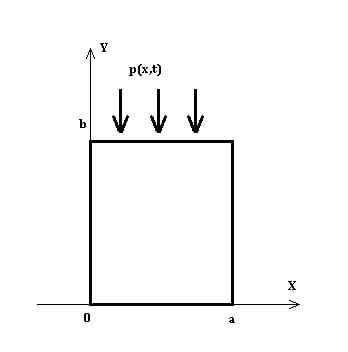
\includegraphics[scale=1]{images/geometry/image_2.jpg}
    \end{center}
    \caption{Геометрія проблеми}\label{geom_gen}
\end{figure}
Розглядається пружна прямокутна область (Рис: \ref{geom_gen}), яка займає область, що у декартовій системі координат описується співвідношенням $0 \le x \le a$, $0 \le y \le b$.

До прямокутної області на грані $y=b$ додане нормальне навантаження
\begin{equation}
    \sigma_y(x, y, t) |_{y=b} = -p(x, t), \quad  \tau_{xy}(x,y,t) |_{y=b} =0, \quad 0 \le x \le a
\end{equation}
де $p(x, t)$ відома функція.
На нижній грані виконуються наступні умови
\begin{equation}
    v(x,y,t) |_{y=0}, \quad \tau_{xy}(x,y,t) |_{y=0} =0
\end{equation}
На бічних гранях $x=0$ та $x=a$ граничні умови запишемо у формі
\begin{equation}\label{gen_bound_gen}
    U_1[f(x,y,t)]=0, \quad U_2[f(x,y,t)]=0 , \quad 0 \le y \le b
\end{equation}
Де 
\begin{align*}
    &U_1[f(x,y,t)]=\left[\alpha_1f(x,y,t) + \beta_1 \frac{\partial f(x,y,t)}{\partial x} \right]|_{x=0} \\
    &U_2[f(x,y,t)]=\left[\alpha_2f(x,y,t) + \beta_2 \frac{\partial f(x,y,t)}{\partial x} \right]|_{x=a} \\
\end{align*}
граничні функціонали у загальному виді (для кожної конкретної задачі вони будуть деталізовані), $f(x,y,t)=(u(x,y,t), v(x,y,t))^T$ - вектор переміщеннь.

Розглядаються наступні рівняння рівноваги Ламе:
\begin{equation}
    \begin{cases}
        \frac{\partial^2 u(x,y,t)}{\partial x^2} + \frac{\partial^2 u(x,y,t)}{\partial y^2} + \mu_0 (\frac{\partial^2 u(x,y,t)}{\partial x^2} + \frac{\partial^2 v(x,y,t)}{\partial x\partial y}) = \frac{1}{c_1^2} \frac{\partial^2 u(x,y,t)}{\partial t^2} \\
        \frac{\partial^2 v(x,y,t)}{\partial x^2} + \frac{\partial^2 v(x,y,t)}{\partial y^2} + \mu_0 (\frac{\partial^2 u(x,y,t)}{\partial x \partial y} + \frac{\partial^2 v(x,y,t)}{\partial y^2}) = \frac{1}{c_2^2} \frac{\partial^2 v(x,y,t)}{\partial t^2} \\
    \end{cases}
\end{equation}

Будемо розглядати випадок гармонічних коливань, тому можемо предствавити функції у наступному вигляді:
\begin{equation}
    u(x,y,t) = u(x,y) e^{i \omega t}, \quad v(x,y,t) = v(x,y) e^{i \omega t}, \quad p(x,t) = p(x) e^{i \omega t}
\end{equation}
Таким чином отримаємо наступні рівняння рівноваги:
\begin{equation}\label{lame_gen}
    \begin{cases}
        \frac{\partial^2 u(x,y)}{\partial x^2} + \frac{\partial^2 u(x,y)}{\partial y^2} + \mu_0 (\frac{\partial^2 u(x,y)}{\partial x^2} + \frac{\partial^2 v(x,y)}{\partial x\partial y}) = -\frac{\omega^2}{c_1^2}  u(x,y) \\
        \frac{\partial^2 v(x,y)}{\partial x^2} + \frac{\partial^2 v(x,y)}{\partial y^2} + \mu_0 (\frac{\partial^2 u(x,y)}{\partial x \partial y} + \frac{\partial^2 v(x,y)}{\partial y^2}) = -\frac{\omega^2}{c_2^2} v(x,y) \\
    \end{cases}
\end{equation}
Та граничні умови:
\begin{equation}\label{bound_gen}
    \begin{cases}
        \sigma_y(x, y) |_{y=b} = -p(x), \quad  \tau_{xy}(x,y) |_{y=b} =0 \\
        v(x,y) |_{y=0}, \quad \tau_{xy}(x,y) |_{y=0} =0 \\
        U_1[f(x,y)]=0, \quad U_2[f(x,y)]=0
    \end{cases}
\end{equation}

Введемо невідомі функції $\chi_1(y) = u(0, y)$, $\chi_2(y) = v(0, y)$, $\chi_3(y) = u(a, y)$, $\chi_4(y) = v(a, y)$.
Враховучи умову \eqref{gen_bound_gen}, отримаємо, що 
$\frac{\partial u(0, y)}{\partial x}=-\frac{\alpha_1}{\beta_1} \chi_1(y)$,
$\frac{\partial v(0, y)}{\partial x}=-\frac{\alpha_1}{\beta_1} \chi_2(y)$,
$\frac{\partial u(a, y)}{\partial x}=-\frac{\alpha_2}{\beta_2} \chi_3(y)$,
$\frac{\partial v(a, y)}{\partial x}=-\frac{\alpha_2}{\beta_2} \chi_4(y)$.
Отже умова \eqref{gen_bound_gen} виконується автоматично.

\subsection{Зведеня задачі до одновимірної у просторі трансформант}
Для того, щоб звести задачу до одновимірної задачі, використаєм інтегральне перетворення Фур'є по змінній $x$ у до рівнянь \eqref{lame_gen} наступному вигляді:
\begin{equation}
    \begin{pmatrix}
        u_n(y) \\
        v_n(y)
    \end{pmatrix} = \int_{0}^{a} 
    \begin{pmatrix}
        u(x,y) sin(\alpha_n x) \\
        v(x,y) cos(\alpha_n x)
    \end{pmatrix} dx, \quad \alpha_n = \frac{\pi n}{a}
\end{equation}

Для цього помножим перше та друге рівняння \eqref{lame_gen} на $sin(\alpha_n x)$ та $cos(\alpha_n x)$ відповідно та проінтегруєм по змінній $x$ на інтервалі $0 \le x \le a$.
Покрокове інтегрування рівняння \eqref{lame_gen} наведено у (\nameref{ap_A}).
Отримана система рівнянь задачі у просторі трансформант:
\begin{equation}\label{transf_gen}
    \begin{cases}
        u_n^{''}(y) - \alpha_n \mu_0 v_n^{'}(y) - (\alpha_n^2 + \alpha_n^2 \mu_0 - \frac{\omega^2}{c_1^2}) u_n(y) = \\
        = \alpha_n(1 + \mu_0)(\chi_3(y) cos(\alpha_n a) - \chi_1(y)) \\
        \\
        (1 + \mu_0) v_n^{''}(y) + \alpha_n \mu_0 u_n^{'}(y) - (\alpha_n^2 - \frac{\omega^2}{c_2^2}) v_n(y) = \\
        = (\frac{\alpha_2}{\beta_2}\chi_4(y) cos(\alpha_n a) - \frac{\alpha_1}{\beta_1}\chi_2(y)) - \mu_0 (\chi_3^{'}(y) cos(\alpha_n a) -\chi_1^{'}(y))
    \end{cases}
\end{equation}

Застосовуючи інтегральне перетворення до граничних умов,
отримаємо наступні умови задачі у просторі трансформант
\begin{equation}\label{transf_bound_gen}
    \begin{cases}
        \left( (2G + \lambda)v_n^{'}(y) + \alpha_n \lambda u_n(y) \right)|_{y=b} = -p_n \\
        \left(u_n^{'}(y) - \alpha_n v_n(y)  \right)|_{y=b} = 0 \\
        v_n(y)|_{y=0} = 0 \\
        \left(u_n^{'}(y) - \alpha_n v_n(y)  \right)|_{y=0} = 0
    \end{cases}
\end{equation}
Де $p_n = \int_{0}^{a} p(x) cos(\alpha_n x) dx$

\subsection{Зведення задачі у просторі трансформант до матрично-векторної форми}
Для того щоб розв'язати задачу у простосторі трансформант, перепишмо її у матрично-векторній формі.
Рівняння рівноваги \eqref{transf_gen} запишемо у наступному вигляді:
\begin{align}\label{transf_mat_gen}
    &L_2\left[ Z_n(y) \right] = A * Z_n^{''}(y) + B * Z_n^{'}(y) + C * Z_n(y) \nonumber \\
    &L_2\left[ Z_n(y) \right] = F_n(y)
\end{align}
Де
\begin{equation*}
    A = \begin{pmatrix}
        1 & 0 \\
        0 & 1 + \mu_0
    \end{pmatrix}, \quad
    B = \begin{pmatrix}
        0 & -\alpha_n \mu_0 \\
        \alpha_n \mu_0 & 0
    \end{pmatrix}
\end{equation*}
\begin{equation*}
    C = \begin{pmatrix}
        -\alpha_n^2 -\alpha_n^2 \mu_0 + \frac{\omega^2}{c_1^2} & 0 \\
        0 & -\alpha_n^2 + \frac{\omega^2}{c_2^2}
    \end{pmatrix}, \quad
    Z_n(y) = \begin{pmatrix}
        u_n(y) \\
        v_n(y)
    \end{pmatrix}
\end{equation*}
\begin{equation*}
    F_n(y) = \begin{pmatrix}
        \alpha_n(1 + \mu_0)(\chi_3(y) cos(\alpha_n a) - \chi_1(y)) \\
        (\frac{\alpha_2}{\beta_2}\chi_4(y) cos(\alpha_n a) - \frac{\alpha_1}{\beta_1}\chi_2(y)) - \mu_0 (\chi_3^{'}(y) cos(\alpha_n a) -\chi_1^{'}(y))
    \end{pmatrix}
\end{equation*}
Граничні умови \eqref{transf_bound_gen} запишемо у наступному вигляді:
\begin{align}\label{transf_bound_mat_gen}
    &U_i\left[ Z_n(y) \right] = E_i * Z_n^{'}(b_i) + F_i * Z_n(b_i) \nonumber \\
    &U_i\left[ Z_n(y) \right] = D_i
\end{align}
Де $i = \overline{0, 1}$, $b_0 = b$, $b_1 = 0$,
\begin{equation*}
    E_0 = \begin{pmatrix}
        1 & 0 \\
        0 & 2G + \lambda
    \end{pmatrix}, \quad
    F_0 = \begin{pmatrix}
        0 & -\alpha_n \\
        \alpha_n \lambda & 0
    \end{pmatrix}, \quad
\end{equation*}
\begin{equation*}
    E_1 = \begin{pmatrix}
        1 & 0 \\
        0 & 0
    \end{pmatrix}, \quad
    F_1 = \begin{pmatrix}
        0 & -\alpha_n \\
        0 & 1
    \end{pmatrix}, \quad
\end{equation*}
\begin{equation*}
    D_0 = \begin{pmatrix}
        0 \\
        -p_n
    \end{pmatrix}, \quad
    D_1 = \begin{pmatrix}
        0 \\
        0
    \end{pmatrix}, \quad
\end{equation*}

Для знаходження розв'язку задачі у просторі трансформант, знайдем фундаментальну матрицю рівняння \eqref{transf_mat_gen}.
Шукати її будем у наступному вигляді:
\begin{equation}
    Y(y) = \frac{1}{2\pi i} \oint_C e^{sy} M^{-1}(s)ds
\end{equation}
Де $M(s)$ - характерестична матриця рівняння \eqref{transf_mat_gen}, а $C$ - замкнений контур який містить усі особливі точки $M^{-1}(s)$. $M(s)$ будемо шукати з наступної умовни
\begin{equation}
    L_2\left[ e^{sy}*I \right] = e^{sy} * M(s), \quad I = \begin{pmatrix} 1 & 0 \\ 0 & 1 \end{pmatrix}
\end{equation}
\begin{align*}
    &L_2\left[ e^{sy}*I \right] = e^{sy} \left( s^2A * I + s B*I + C*I \right) = \\
    &=e^{sy} \begin{pmatrix}
        s^2 - \alpha_n^2 - \alpha_n^2\mu_0 + \frac{\omega^2}{c_1^2} & -\alpha_n \mu_0 s \\
        \alpha_n \mu_0 s & s^2 (1 + \mu_0) -\alpha_n^2 + \frac{\omega^2}{c_1^2}
     \end{pmatrix} =>
\end{align*}

\begin{equation}
    M(s) = \begin{pmatrix}
        s^2 - \alpha_n^2 - \alpha_n^2\mu_0 + \frac{\omega^2}{c_1^2} & -\alpha_n \mu_0 s \\
        \alpha_n \mu_0 s & s^2 (1 + \mu_0) -\alpha_n^2 + \frac{\omega^2}{c_2^2}
     \end{pmatrix}
\end{equation}

Знайдемо тепер $M^{-1}(s) = \frac{\widetilde{M(s)}}{det[M(s)]}$.
\begin{equation}
    \widetilde{M(s)} = \begin{pmatrix}
        s^2 (1 + \mu_0) -\alpha_n^2 + \frac{\omega^2}{c_2^2} & \alpha_n \mu_0 s \\
        -\alpha_n \mu_0 s & s^2 - \alpha_n^2 - \alpha_n^2\mu_0 + \frac{\omega^2}{c_1^2}
     \end{pmatrix}
\end{equation}
\begin{align}
    &det[M(s)] = \begin{vmatrix}
        s^2 - \alpha_n^2 - \alpha_n^2\mu_0 + \frac{\omega^2}{c_1^2} & -\alpha_n \mu_0 s \\
        \alpha_n \mu_0 s & s^2 (1 + \mu_0) -\alpha_n^2 + \frac{\omega^2}{c_2^2}
     \end{vmatrix} = \nonumber \\
    &=(s - s_1)(s + s_1)(s - s_2)(s + s_2)
\end{align}
Де $s_1$, $s_2$, $-s_1$, $-s_2$ корені $det[M(s)]=0$, детальне знаходження яких наведено в (\nameref{ap_B}).

Враховучи це, тепер знайдемо значення фундаментальної матрицю за допомогою теореми про лишки:
\begin{align*}
    &\frac{1}{2\pi i} \oint_C e^{sy} M^{-1}(s)ds = \frac{2 \pi i}{2 \pi i (1 + \mu_0)} \sum_{i=1}^{4} Res\left[ e^{sy} \frac{\widetilde{M(s)}}{det[M(s)]} \right] = \\
    & = \left(Y_0(y) + Y_1(y) + Y_2(y) + Y_3(y) \right)
\end{align*}
Знайдем $Y_0(y)$:
\begin{align}
    &Y_0(y) =  \left( \frac{e^{sy}}{(s+s_1)(s - s_2)(s + s_2)} \widetilde{M(s)} \right) \Big|_{s=s_1} = \nonumber \\
    &=\frac{e^{s_1 y}}{2s_1 (s_1^2 - s_2^2)} \begin{pmatrix}
        s_1^2 (1 + \mu_0) -\alpha_n^2 + \frac{\omega^2}{c_2^2} & \alpha_n \mu_0 s_1 \\
        -\alpha_n \mu_0 s_1 & s_1^2 - \alpha_n^2 - \alpha_n^2\mu_0 + \frac{\omega^2}{c_1^2}
    \end{pmatrix}
\end{align}
Знайдем $Y_1(y)$:
\begin{align}
    &Y_1(y) =  \left( \frac{e^{sy}}{(s-s_1)(s - s_2)(s + s_2)} \widetilde{M(s)} \right) \Big|_{s=-s_1} = \nonumber \\
    &=-\frac{e^{-s_1 y}}{2s_1 (s_1^2 - s_2^2)} \begin{pmatrix}
        s_1^2 (1 + \mu_0) -\alpha_n^2 + \frac{\omega^2}{c_2^2} & -\alpha_n \mu_0 s_1 \\
        \alpha_n \mu_0 s_1 & s_1^2 - \alpha_n^2 - \alpha_n^2\mu_0 + \frac{\omega^2}{c_1^2}
    \end{pmatrix}
\end{align}
Знайдем $Y_2(y)$:
\begin{align}
    &Y_2(y) =  \left( \frac{e^{sy}}{(s+s_2)(s - s_1)(s + s_1)} \widetilde{M(s)} \right) \Big|_{s=s_2} = \nonumber \\
    &=\frac{e^{s_2 y}}{2s_2 (s_2^2 - s_1^2)} \begin{pmatrix}
        s_2^2 (1 + \mu_0) -\alpha_n^2 + \frac{\omega^2}{c_2^2} & \alpha_n \mu_0 s_2 \\
        -\alpha_n \mu_0 s_2 & s_2^2 - \alpha_n^2 - \alpha_n^2\mu_0 + \frac{\omega^2}{c_1^2}
    \end{pmatrix}
\end{align}
Знайдем $Y_3(y)$:
\begin{align}
    &Y_3(y) =  \left( \frac{e^{sy}}{(s-s_2)(s - s_1)(s + s_1)} \widetilde{M(s)} \right) \Big|_{s=-s_2} = \nonumber \\
    &=-\frac{e^{-s_2 y}}{2s_2 (s_2^2 - s_1^2)} \begin{pmatrix}
        s_2^2 (1 + \mu_0) -\alpha_n^2 + \frac{\omega^2}{c_2^2} & -\alpha_n \mu_0 s_2 \\
        \alpha_n \mu_0 s_2 & s_2^2 - \alpha_n^2 - \alpha_n^2\mu_0 + \frac{\omega^2}{c_1^2}
    \end{pmatrix}
\end{align}

\subsection{Побудова матриці-функції Гріна}
Для побудови матриці-функції Гріна спочатку знайдем тепер фундамельні бизисні матриці $\Psi_0(y)$, $\Psi_1(y)$, шукати їх будем у наступному вигляді:
\begin{equation}\label{psi_gen}
    \Psi_i(y) = \left( Y_0(y) + Y_1(y) \right) * C_1^i + \left( Y_2(y) + Y_3(y) \right) * C_2^i
\end{equation}

Залишилось знайти невідомі матриці коєфіцієнтів $C_1^0$, $C_2^0$, $C_1^1$, $C_2^1$ використовуючи граничні умови \eqref{transf_bound_mat_gen}.
Покрокове знаходження яких наведено у (\nameref{ap_C}).
Для подальшого введемо наступні позначення для елементів матриць $\Psi_0(y)$, $\Psi_1(y)$:
\begin{equation*}
    \Psi_0(y) = \begin{pmatrix}
        \Psi_1^0(y) &  \Psi_2^0(y) \\
        \Psi_3^0(y) &  \Psi_4^0(y) 
    \end{pmatrix}, \quad 
    \Psi_1(y) = \begin{pmatrix}
        \Psi_1^1(y) &  \Psi_2^1(y) \\
        \Psi_3^1(y) &  \Psi_4^1(y) 
    \end{pmatrix}      
\end{equation*}

Таким чином матрицю Гріна можемо записати у вигляді:
\begin{equation}
    G(y,\xi) = 
    \begin{cases}
        \Psi_0(y) * \Psi_1(\xi), \quad 0 \le y < \xi \\
        \Psi_1(y) * \Psi_0(\xi), \quad \xi < y \le b
    \end{cases}
\end{equation}

Для данної матриці Гріна виконано усі властивості, зокрема виконані однорідні граничні умови \eqref{transf_bound_mat_gen}
та однорідні рівняння рівноваги у просторі трансформант \eqref{transf_mat_gen}:
\begin{equation*}
    L_2\left[  G(y, \xi) \right] = 0
\end{equation*}
\begin{equation*}
    U_0\left[ G(y, \xi) \right] = 0, \quad  U_1\left[ G(y, \xi) \right],
\end{equation*}

Таким чином ми можемо записати розв'язок крайової задачі у просторі трансформант:
\begin{equation}
    Z_n(y) = \int_0^b G(y,\xi) F_n(\xi) d\xi + \Psi_0(y) * D_0 + \Psi_1(y) * D_1
\end{equation}

Введемо наступні позначення $G(y, \xi) = \begin{pmatrix}
    g_1(y,\xi) & g_2(y,\xi) \\
    g_3(y,\xi) & g_4(y,\xi)
\end{pmatrix}$, $F_n(y) = \begin{pmatrix}
    f_n^1(y) \\
    f_n^2(y)
\end{pmatrix}$, $\Psi_i(y) = \begin{pmatrix}
    \psi_i^1(y) & \psi_i^2(y) \\
    \psi_i^3(y) & \psi_i^4(y)
\end{pmatrix}$, $i=0,1$. Враховуючи це, шукані функціі перемішень у просторі трансформант можна записати у наступному вигляді
\begin{align}\label{transf_sol_u_gen}
    &u_n(y) = \int_0^b \left[g_1(y, \xi)f_n^1(\xi) + g_2(y, \xi)f_n^2(\xi) \right]d\xi - \psi_0^2(y) p_n
\end{align}
\begin{align}\label{transf_sol_v_gen}
    &v_n(y) = \int_0^b \left[g_3(y, \xi)f_n^1(\xi) + g_4(y, \xi)f_n^2(\xi) \right]d\xi - \psi_0^4(y) p_n
\end{align}

\subsection{Побудова розв'язоку вихідної задачі}
Викорустовуючи обернене інтегральне перетворення Фур'є до розв'язку задачі у просторі трансформант
(\ref{transf_sol_u_gen}), (\ref{transf_sol_v_gen}), отримаємо фінальний розв'язок задачі
\begin{equation}
    u(x,y) = \frac{2}{a} \sum_{n=1}^{\infty} u_n(y) sin(\alpha_n x), \quad \alpha_n = \frac{\pi n}{a}
\end{equation}
\begin{equation}
    v(x,y) = \frac{v_0(y)}{a} + \frac{2}{a} \sum_{n=1}^{\infty} v_n(y) cos(\alpha_n x), \quad \alpha_n = \frac{\pi n}{a}
\end{equation}

Знайдем тепер $v_0(y)$ розглянувши задачу у просторі трансформант \eqref{transf_gen}, \eqref{transf_bound_gen} при $n=0$, $\alpha_n = 0$.
Детальний розв'язок якої наведено в (\nameref{ap_D}). Тоді остаточний розв'язок $v(x,y)$ буде мати вигляд
\begin{align}
    &v(x,y) = \frac{2}{a} \sum_{n=1}^{\infty} v_n(y) cos(\alpha_n x) - \psi_0(y) \frac{p_0}{a(2G + \lambda)} + \\
    &+ \frac{1}{a(1+\mu_0)} \int_{0}^{b}g(y,\xi) \left[ (\frac{\alpha_2}{\beta_2}\chi_4(\xi) cos(\alpha_n a) - \frac{\alpha_1}{\beta_1}\chi_2(\xi)) - \frac{\mu_0}{(1+\mu_0)} (\chi_3^{'}(\xi) cos(\alpha_n a) -\chi_1^{'}(\xi)) \right] d\xi
\end{align}

Залишилось знайти невідомі функції $\chi_1(y)$, $\chi_2(y)$, $\chi_3(y)$, $\chi_4(y)$.
В подальшому в данній роботі розглянуто випадок таких граничних умов які призводять лише до однієї невідомої функції $f(y) = \frac{\partial v(x,y)}{\partial x}|_{x=a}$.
Для знаходження якої буде побудовано інтегральне рівняння завдяки граничній умові $\sigma_y(x, y) |_{y=b} = -p(x)$.

\subsection{Загальна схема розв'язку сінгулярного інтегрального рівняння}
Розглянемо випадок граничних умов другої основної задачі теорії пружності, в результаті отримаємо лише одну невідому функцію $f(y) = \frac{\partial v(x,y)}{\partial x}|_{x=a}$.
З цього отримаємо значення $f_n^1(\xi) = 0$, $f_n^2(\xi)= -cos(\alpha_n a) f(\xi) $
Запишем тепер фінальний розв'язок для цього випадку:
\begin{equation}
    u(x,y) = -\frac{2}{a} \sum_{n=1}^{\infty} \left( \int_0^b \left[g_2(y, \xi)cos(\alpha_n a) f(\xi) \right]d\xi + \psi_0^2(y) p_n \right) sin(\alpha_n x), \quad \alpha_n = \frac{\pi n}{a}
\end{equation}
\begin{align}
    &v(x,y) = -\frac{1}{a(1+\mu_0)} \int_{0}^{b}g(y,\xi) f(\xi) d\xi - \psi_0(y) \frac{p_0}{a(2G + \lambda)} \\
    &- \frac{2}{a} \sum_{n=1}^{\infty} \left( \int_0^b \left[g_4(y, \xi) cos(\alpha_n a) f(\xi) \right]d\xi + \psi_0^4(y) p_n  \right) cos(\alpha_n x), \quad \alpha_n = \frac{\pi n}{a}
\end{align}

Використиєм граничну умову $\sigma_y(x, y) |_{y=b} = -p(x)$ для того, щоб отримати інтегральне рівняння:
\begin{equation*}
    (2G + \lambda)\frac{\partial v(x,y)}{\partial y}|_{y=b} + \lambda\frac{\partial u(x,y)}{\partial x}|_{y=b} = -p(x) \Leftrightarrow
\end{equation*}
\begin{align*}
    &-\frac{(2G + \lambda)}{a(1+\mu_0)} \int_{0}^{b}\frac{\partial g(y, \xi)}{\partial y}|_{y=b} f(\xi) d\xi - \psi_0^{'}(b) \frac{p_0}{a} - \\
    &- \frac{2(2G + \lambda)}{a} \frac{\partial}{\partial y} \sum_{n=1}^{\infty} \left( \int_0^b \left[g_4(y, \xi) cos(\alpha_n a) f(\xi) \right]d\xi + \psi_0^{4}(y) p_n \right) cos(\alpha_n x)|_{y=b} - \\
    & -\frac{2\lambda}{a} \frac{\partial}{\partial x} \sum_{n=1}^{\infty} \left( \int_0^b \left[g_2(y, \xi)cos(\alpha_n a) f(\xi) \right]d\xi + \psi_0^2(y) p_n \right) sin(\alpha_n x)|_{y=b} = -p(x)
\end{align*}
Введемо позначення:
\begin{equation}
    a_1(x) = a p(x) - \left[ 2(2G + \lambda) \frac{\partial}{\partial y} \sum_{n=1}^{\infty} \psi_0^{4}(y) p_n cos(\alpha_n x) + 2\lambda \frac{\partial}{\partial x} \sum_{n=1}^{\infty}\psi_0^2(y) p_n sin(\alpha_n x) + \psi_0^{'}(b) p_0\right]|_{y=b}
\end{equation}
Враховуючи його отримаємо наступне інтегральне рівняння відносно $f(\xi)$:
\begin{align}\label{int_gen}
    &\frac{(2G + \lambda)}{(1+\mu_0)} \int_{0}^{b}\frac{\partial g(y, \xi)}{\partial y}|_{y=b} f(\xi) d\xi + \\ 
    &+ \int_{0}^{b} \sum_{n=1}^{\infty} cos(\alpha_n a) cos(\alpha_n x) \left[(2G + \lambda) \frac{\partial g_4(y, \xi)}{\partial y} + \alpha_n \lambda g_2(y, \xi) \right]|_{y=b} f(\xi) d\xi = a_1(x)
\end{align}
Розглянемо ряд:
\begin{align*}
    &\sum_{n=1}^{\infty} cos(\alpha_n a) cos(\alpha_n x) \left[(2G + \lambda) \frac{\partial g_4(y, \xi)}{\partial y} + \alpha_n \lambda g_2(y, \xi) \right]|_{y=b} = \\
    &= \sum_{n=1}^{\infty} (-1)^n \alpha_n^{-1} e^{\alpha_n (\xi - b)} cos(\alpha_n x) \left[ \frac{\partial \widetilde{g_4(y, \xi)}}{\partial y} + \lambda \widetilde{g_2(y, \xi)} \right]|_{y=b} = \\
    &= \sum_{n=1}^{N} (-1)^n \alpha_n^{-1} e^{\alpha_n (\xi - b)} cos(\alpha_n x) \left[ \frac{\partial \widetilde{g_4(y, \xi)}}{\partial y} + \lambda \widetilde{g_2(y, \xi)} \right]|_{y=b} + \\
    & + a_2 \sum_{n=N}^{\infty} (-1)^n (2n + 1)^{-1} e^{-(2n + 1) \frac{\pi}{2a} (b - \xi)} cos((2n + 1) \frac{\pi}{2a} x) + \\
    & + a_2 \sum_{n=0}^{N} (-1)^n (2n + 1)^{-1} e^{-(2n + 1) \frac{\pi}{2a} (b - \xi)} cos((2n + 1) \frac{\pi}{2a} x) - \\
    & - a_2 \sum_{n=0}^{N} (-1)^n (2n + 1)^{-1} e^{-(2n + 1) \frac{\pi}{2a} (b - \xi)} cos((2n + 1) \frac{\pi}{2a} x) = \\
    &= a_2 \sum_{n=0}^{\infty} (-1)^n (2n + 1)^{-1} e^{-(2n + 1) \frac{\pi}{2a} (b - \xi)} cos((2n + 1) \frac{\pi}{2a} x) + a_3(\xi, x)
\end{align*}

Використовуючи формулу 5.4.12.8 \cite{prudnikov} отримаємо:
\begin{align*}
    &a_2 \sum_{n=0}^{\infty} (-1)^n (2n + 1)^{-1} e^{-(2n + 1) \frac{\pi}{2a} (b - \xi)} cos((2n + 1) \frac{\pi}{2a} x) + a_3(\xi, x) = \\
    &= \frac{a_2}{4} ln\left[ \frac{ch(\frac{\pi}{2a}(b - \xi)) + cos(\frac{\pi}{2a}x)}{ch(\frac{\pi}{2a}(b - \xi)) - cos(\frac{\pi}{2a}x)} \right] + a_3(\xi, x)
\end{align*}

Де:
\begin{equation*}
    a_2 = \frac{2}{\pi} \lim_{n \rightarrow \infty}\left[ \frac{\partial \widetilde{g_4(y, \xi)}}{\partial y} + \lambda \widetilde{g_2(y, \xi)} \right]|_{y=b}, 
\end{equation*}
\begin{align*}
    &a_3(\xi, x) = \sum_{n=1}^{N} cos(\alpha_n a) cos(\alpha_n x) \left[(2G + \lambda) \frac{\partial g_4(y, \xi)}{\partial y} + \alpha_n \lambda g_2(y, \xi) \right]|_{y=b} - \\
    & - a_2 \sum_{n=0}^{N} (-1)^n (2n + 1)^{-1} e^{-(2n + 1) \frac{\pi}{2a} (b - \xi)} cos((2n + 1) \frac{\pi}{2a} x)
\end{align*}

Повернемося до інтегралу
\begin{align}
    &\frac{(2G + \lambda)}{(1+\mu_0)} \int_{0}^{b}\frac{\partial g(y, \xi)}{\partial y}|_{y=b} f(\xi) d\xi + \int_{0}^{b} \left( \frac{a_2}{4} ln\left[ \frac{ch(\frac{\pi}{2a}(b - \xi)) + cos(\frac{\pi}{2a}x)}{ch(\frac{\pi}{2a}(b - \xi)) - cos(\frac{\pi}{2a}x)} \right] + a_3(\xi, x) \right) f(\xi) d\xi = \\
    & = \int_{0}^{b} \left( \frac{a_2}{4} ln\left[ \frac{ch(\frac{\pi}{2a}(b - \xi)) + cos(\frac{\pi}{2a}x)}{ch(\frac{\pi}{2a}(b - \xi)) - cos(\frac{\pi}{2a}x)} \right] + a_3(\xi, x) + \frac{(2G + \lambda)}{(1+\mu_0)} \frac{\partial g(y, \xi)}{\partial y}|_{y=b} \right) f(\xi) d\xi = \\
    &= \left[
        \begin{matrix}
            t = \frac{ch(\frac{\pi}{2a}(b - \xi)) - 1}{1 - ch(\frac{\pi b}{2a})} \\
            sh(\frac{\pi}{2a}(b - \xi))d\xi = -\frac{2a}{\pi} (ch(\frac{\pi b}{2a}) - 1) dt \\
            \xi = 0, \quad t = 1 \\
            \xi = b, \quad t = 0 \\
            \xi = b - \frac{2a}{\pi} arch((ch(\frac{\pi b}{2a}) - 1)t + 1)
        \end{matrix}
        \right] = \\
    &=a_5 \int_{0}^{b} a_4(t) \left( \frac{a_2}{4} ln\left[ \frac{t + cos(\frac{\pi}{2a}x)}{t - cos(\frac{\pi}{2a}x)} \right] + \widetilde{a_3(t, x)} \right) \widetilde{f(t)} dt
\end{align}
Де:
\begin{align*}
    &\widetilde{a_3(t, x)} = a_3\left(b - \frac{2a}{\pi} arch((ch(\frac{\pi b}{2a}) - 1)t + 1), x \right) + \frac{(2G + \lambda)}{(1+\mu_0)} \frac{\partial g(y, b - \frac{2a}{\pi} arch((ch(\frac{\pi b}{2a}) - 1)t + 1))}{\partial y}|_{y=b} \\
    &f(t) = f(b - \frac{2a}{\pi} arch((ch(\frac{\pi b}{2a}) - 1)t + 1)) \\
    &a_4(t) = \frac{1}{ sh\left(arch\left[ (ch(\frac{\pi b}{2a}) - 1)t + 1 \right]\right) } \\
    &a_5 = \frac{2a}{\pi} (ch(\frac{\pi b}{2a}) - 1)
\end{align*}

Таким чином отримаємо наступне інтегральне рівняння:
\begin{equation}
    a_5 \int_{0}^{b} a_4(t) \left( \frac{a_2}{4} ln\left[ \frac{t + cos(\frac{\pi}{2a}x)}{t - cos(\frac{\pi}{2a}x)} \right] + \widetilde{a_3(t, x)} \right) \widetilde{f(t)} dt = a_1(x)
\end{equation}


\subsection{Висновки до другого розділу}
Безпосередньо застосовані інтегральні перетворення до рівнянь рівноваги Ламе та крайових умов плоскої задачі теорії пружності для прямокутної області.
Це дозволило уникнути використання допоміжних гармонічних або бігармонічних функцій.
Зведено вихідну задачу до одновимірної векторної крайової задачі у просторі трансформант.
Цю задачу було розв'язано за допомогою методів диференціального матричного числення.
Для цього була побудована фундаментальна базисна матрична система розв'язків однорідного матричного рівняння та матриця-функція Гріна для диференціального векторного рівняння другого порядку.
Побудовано та розв'язано сінгульрне інтегральне рівняння відносно невідомої функції шляхом викорстання методу ортагональних поліномів, та зведення рівнняння до бескінечної алгебричної системи,
яка в подальшому була розв'язана методом редукціі.

\newpage

\section[МІШАНА ЗАДАЧА ТЕОРІЇ ПРУЖНОСТІ ДЛЯ ПРЯМОКУТНОЇ ОБЛАСТІ ЗА УМОВ ІДЕАЛЬНОГО КОНТАКТУ НА БІЧНИХ ГРАНЯХ]
{\centering МІШАНА ЗАДАЧА ТЕОРІЇ ПРУЖНОСТІ ДЛЯ ПРЯМОКУТНОЇ ОБЛАСТІ ЗА УМОВ ІДЕАЛЬНОГО КОНТАКТУ НА БІЧНИХ ГРАНЯХ}
У даному розділі досліджено плоскі статична та динамічна задачі теорії пружності для прямокутної області,
за умов ідеального контакту на бічних гранях.

Вихідні задачі зведено до одновимірної задачі у просторі трансформант за допомогою інтегрального перетворення Фур'є.
Отримані крайові задачі розв'язано точно за допомогою методу матричного диференціального числення.
Остаточне подання для полів переміщень та напружень наведено за допомогою оберненного перетворення Фур'є.

Проведено чисельний аналіз отриманих функцій переміщень та напружень для різних розмірів прямокутної області та різних видів навантаження.

Результати розділу опубліковані в \cite{pozhylenkov_1}, \cite{pozhylenkov_2}, \cite{pozhylenkov_3}, \cite{pozhylenkov_5}
а також доповідались на конференціях \cite{conf_1}, \cite{conf_2}, \cite{conf_4}.
\subsection{Статична задача теорії пружності для прямокутної області за умов ідеального контакту на бічних гранях}
У даному розділі досліджено плоска статична задача теорії пружності для прямокутної області,
за умов ідеального контакту на бічних гранях.

Вихідна задача зведена до одновимірної задачі у просторі трансформант за допомогою інтегрального перетворення Фур'є.
Отримана крайова задача розв'язана точно за допомогою методу матрично диференціального числення,
фундаментальний розв'язок представлений як інтеграл по замкненому контору, який в свою чергу, був знайденний за допомогою теоремі про лишки.
Остаточний вигляд для функцій переміщеннь та напружень отриман шляхом оберненого перетворення Фур'є.

Проведено чисельний аналіз отриманих функцій переміщень та напружень для різних розмірів прямокутної області та різних видів навантаження.

\subsection{Постановка задачі}
\begin{figure}[h]
    \begin{center}
        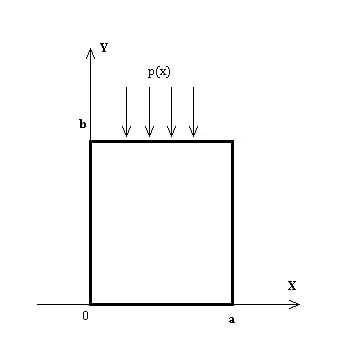
\includegraphics[scale=1]{images/geometry/image_3.jpg}
    \end{center}
    \caption{Геометрія проблеми}\label{geom_static_1}
\end{figure}
Розглядається пружна прямокутна область (Рис: \ref{geom_static_1}), яка займає облась,
що описується у декартовій системі координат співвідношенням $0 \le x \le a$, $0 \le y \le b$.

До прямокутної області на грані $y=b$ додане нормальне навантаження
\begin{equation}
    \sigma_y(x, y) |_{y=b} = -p(x), \quad  \tau_{xy}(x,y) |_{y=b} =0
\end{equation}
де $p(x)$ відома функція.

На бічних гранях виконується умова ідеального контакту
\begin{equation}\label{bound_1_static_1}
    u(x,y) |_{x=0} = 0, \quad \tau_{xy}(x,y) |_{x=0} =0
\end{equation}
\begin{equation}\label{bound_2_static_1}
    u(x,y) |_{x=a} = 0, \quad \tau_{xy}(x,y) |_{x=a} =0
\end{equation}
На нижній грані виконуються наступні умови
\begin{equation}
    v(x,y) |_{y=0} = 0, \quad \tau_{xy}(x,y) |_{y=0} =0
\end{equation}
Розглядаються наступні рівняння рівноваги Ламе:
\begin{equation}\label{lame_static_1}
    \begin{cases}
        \frac{\partial^2 u(x,y)}{\partial x^2} + \frac{\partial^2 u(x,y)}{\partial y^2} + \mu_0 (\frac{\partial^2 u(x,y)}{\partial x^2} + \frac{\partial^2 v(x,y)}{\partial x\partial y}) = 0 \\
        \frac{\partial^2 v(x,y)}{\partial x^2} + \frac{\partial^2 v(x,y)}{\partial y^2} + \mu_0 (\frac{\partial^2 u(x,y)}{\partial x \partial y} + \frac{\partial^2 v(x,y)}{\partial y^2}) = 0 \\
    \end{cases}
\end{equation}

\subsection{Зведеня задачі до одновимірної у просторі трансформант}
Для того, щоб звести задачу до одновимірної задачі, використаєм інтегральне перетворення Фур'є по змінній $x$ у до рівнянь (\ref{lame_static_1}) наступному вигляді:
\begin{equation}
    \begin{pmatrix}
        u_n(y) \\
        v_n(y)
    \end{pmatrix} = \int_{0}^{a} 
    \begin{pmatrix}
        u(x,y) sin(\alpha_n x) \\
        v(x,y) cos(\alpha_n x)
    \end{pmatrix} dx, \quad \alpha_n = \frac{\pi n}{a}
\end{equation}

Для цього помножим перше та друге рівняння (\ref{lame_static_1}) на $sin(\alpha_n x)$ та $cos(\alpha_n x)$ відповідно та проінтегруєм по змінній $x$ на інтервалі $0 \le x \le a$.
Покрокове інтегрування рівняння (\ref{lame_static_1}) наведено у (\nameref{ap_A}).
Отримана система рівнянь задачі у просторі трансформант:
\begin{equation}\label{transf_static_1}
    \begin{cases}
        u_n^{''}(y) - \alpha_n \mu_0 v_n^{'}(y) - \alpha_n^2 (1 + \mu_0) u_n(y) = 0 \\
        (1 + \mu_0) v_n^{''}(y) + \alpha_n \mu_0 u_n^{'}(y)  - \alpha_n^2 v_n(y) = 0 \\
    \end{cases}
\end{equation}

Застосовуючи інтегральне перетворення до граничних умов,
отримаємо наступні умови задачі у просторі трансформант
\begin{equation}\label{transf_bound_static_1}
    \begin{cases}
        \left( (2G + \lambda)v_n^{'}(y) + \alpha_n \lambda u_n(y) \right)|_{y=b} = -p_n \\
        \left(u_n^{'}(y) - \alpha_n v_n(y)  \right)|_{y=b} = 0 \\
        v_n(y)|_{y=0} = 0 \\
        \left(u_n^{'}(y) - \alpha_n v_n(y)  \right)|_{y=0} = 0
    \end{cases}
\end{equation}
Де $p_n = \int_{0}^{a} p(x) cos(\alpha_n x) dx$

\subsection{Зведення задачі у просторі трансформант до матрично-векторної форми}
Для того щоб розв'язати задачу у простосторі трансформант, перепишмо її у матрично-векторній формі.
Рівняння рівноваги (\ref{transf_static_1}) запишемо у наступному вигляді:
\begin{align}\label{transf_mat_static_1}
    &L_2\left[ Z_n(y) \right] = A * Z_n^{''}(y) + B * Z_n^{'}(y) + C * Z_n(y) \nonumber \\
    & L_2\left[ Z_n(y) \right] = 0
\end{align}
Де
\begin{equation*}
    A = \begin{pmatrix}
        1 & 0 \\
        0 & 1 + \mu_0
    \end{pmatrix}, \quad
    B = \begin{pmatrix}
        0 & -\alpha_n \mu_0 \\
        \alpha_n \mu_0 & 0
    \end{pmatrix}, \quad
    C = \begin{pmatrix}
        -\alpha_n^2(1 + \mu_0) & 0 \\
        0 & -\alpha_n^2
    \end{pmatrix}
\end{equation*}
\begin{equation*}
    Z_n(y) = \begin{pmatrix}
        u_n(y) \\
        v_n(y)
    \end{pmatrix}
\end{equation*}
Граничні умови (\ref{transf_bound_static_1}) запишемо у наступному вигляді:
\begin{align}\label{transf_bound_mat_static_1}
    &U_i\left[ Z_n(y) \right] = E_i * Z_n^{'}(b_i) + F_i * Z_n(b_i) \nonumber \\
    & U_i\left[ Z_n(y) \right] = D_i
\end{align}
Де $i = \overline{0, 1}$, $b_0 = b$, $b_1 = 0$,
\begin{equation*}
    E_0 = \begin{pmatrix}
        1 & 0 \\
        0 & 2G + \lambda
    \end{pmatrix}, \quad
    F_0 = \begin{pmatrix}
        0 & -\alpha_n \\
        \alpha_n \lambda & 0
    \end{pmatrix}, \quad
\end{equation*}
\begin{equation*}
    E_1 = \begin{pmatrix}
        1 & 0 \\
        0 & 0
    \end{pmatrix}, \quad
    F_1 = \begin{pmatrix}
        0 & -\alpha_n \\
        0 & 1
    \end{pmatrix}, \quad
\end{equation*}
\begin{equation*}
    D_0 = \begin{pmatrix}
        0 \\
        -p_n
    \end{pmatrix}, \quad
    D_1 = \begin{pmatrix}
        0 \\
        0
    \end{pmatrix}, \quad
\end{equation*}

Для знаходження розв'язку задачі у просторі трансформант, знайдем фундаментальну матрицю рівняння (\ref{transf_mat_static_1}).
Шукати її будем у наступному вигляді \cite{gantmaher}:
\begin{equation}
    Y(y) = \frac{1}{2\pi i} \oint_C e^{sy} M^{-1}(s)ds
\end{equation}
Де $M(s)$ - характерестична матриця рівняння (\ref{transf_mat_static_1}), а $C$ - замкнений контур який містить усі особливі точки. Яку будемо шукати з наступної умовни
\begin{equation}
    L_2\left[ e^{sy}*I \right] = e^{sy} * M(s), \quad I = \begin{pmatrix} 1 & 0 \\ 0 & 1 \end{pmatrix}
\end{equation}
\begin{align*}
    &L_2\left[ e^{sy}*I \right] = e^{sy} \left( s^2A * I + s B*I + C*I \right) = \\
    &=e^{sy} \left( \begin{pmatrix}
        s^2 & 0 \\
        0 & s^2 (1 + \mu_0)
    \end{pmatrix} + \begin{pmatrix}
        0 & -\alpha_n \mu_0 s\\
        \alpha_n \mu_0 s & 0
    \end{pmatrix} + \begin{pmatrix}
        -\alpha_n^2(1 + \mu_0) & 0 \\
        0 & -\alpha_n^2
    \end{pmatrix} \right) =  \\
    &=e^{sy} \begin{pmatrix}
        s^2 -\alpha_n^2(1 + \mu_0) & -\alpha_n \mu_0 s \\
        \alpha_n \mu_0 s & s^2 (1 + \mu_0) -\alpha_n^2
     \end{pmatrix} =>
\end{align*}

\begin{equation}
    M(s) = \begin{pmatrix}
        s^2 -\alpha_n^2(1 + \mu_0) & -\alpha_n \mu_0 s \\
        \alpha_n \mu_0 s & s^2 (1 + \mu_0) -\alpha_n^2
     \end{pmatrix}
\end{equation}

Знайдемо тепер $M^{-1}(s) = \frac{\widetilde{M(s)}}{det[M(s)]}$.
\begin{equation}
    \widetilde{M(s)} = \begin{pmatrix}
        s^2 (1 + \mu_0) -\alpha_n^2 & \alpha_n \mu_0 s \\
        -\alpha_n \mu_0 s & s^2 -\alpha_n^2(1 + \mu_0)
     \end{pmatrix}
\end{equation}
\begin{align}
    &det[M(s)] = \begin{vmatrix}
        s^2 - \alpha_n^2 - \alpha_n^2\mu_0 & -\alpha_n \mu_0 s \\
        \alpha_n \mu_0 s & s^2 (1 + \mu_0) -\alpha_n^2
     \end{vmatrix} = \nonumber \\
    &=(1+\mu_0)(s - \alpha_n)^2(s + \alpha_n)^2
\end{align}
Де $\alpha_n$, $-\alpha_n$, корені $det[M(s)]=0$, детальне знаходження яких наведено в (\nameref{ap_B}).

Враховучи це, тепер знайдемо значення фундаментальної матрицю за допомогою теореми про лишки:
\begin{align*}
    &\frac{1}{2\pi i} \oint_C e^{sy} M^{-1}(s)ds = \frac{2 \pi i}{2 \pi i (1 + \mu_0)} \sum_{i=1}^{2} Res\left[ e^{sy} \frac{\widetilde{M(s)}}{det[M(s)]} \right] = \\
    & = \frac{1}{(1 + \mu_0)} \left(Y_0(y) + Y_1(y) \right)
\end{align*}
Знайдем $Y_0(y)$:
\begin{align}
    &Y_0(y) =  \frac{\partial}{\partial s} \left( \frac{e^{sy}}{(s+\alpha_n)^2} \widetilde{M(s)} \right) \Big|_{s=\alpha_n} = \nonumber \\
    &=\frac{e^{\alpha_n y}}{4\alpha_n} \begin{pmatrix}
    \alpha_n \mu_0 y + 2 + \mu_0 & \alpha_n \mu_0 y \\
    -\alpha_n \mu_0 y & -\alpha_n \mu_0 y + 2 + \mu_0
    \end{pmatrix}
\end{align}
Знайдем $Y_1(y)$:
\begin{align}
    &Y_1(y) = \frac{\partial}{\partial s} \left(\frac{e^{sy}}{(s-\alpha_n)^2} \widetilde{M(s)} \right) \Big|_{s=-\alpha_n} = \nonumber \\
    =&\frac{e^{-\alpha_n y}}{4\alpha_n} \begin{pmatrix}
    \alpha_n \mu_0 y - 2 - \mu_0 & -\alpha_n \mu_0 y \\
    \alpha_n \mu_0 y & -\alpha_n \mu_0 y - 2 - \mu_0
    \end{pmatrix}
\end{align}

Таким чином ми можемо записати розв'язок задачі у просторі трансформант:
\begin{equation}
    Z_n(y) = \frac{1}{1 + \mu_0} \left( Y_0(y) * \begin{pmatrix} c_1 \\ c_2 \end{pmatrix} +  Y_1(y) * \begin{pmatrix} c_3 \\ c_4 \end{pmatrix}  \right)
\end{equation}
Залишилось знайти невідомі коєфіцієнти $c_1$, $c_2$, $c_3$, $c_4$, використовуючи граничні умови (\ref{transf_bound_mat_static_1}).
Покрокове знаходження коєфіцієнтів наведено у (\nameref{ap_E}).
Таким чином ми можемо записати розв'зок у просторі трансформант:
\begin{align}\label{transf_sol_u_static_1}
    &u_n(y) = \frac{e^{\alpha_n y}}{4 \alpha_n (1 + \mu_0)} \left[c_1 (\alpha_n \mu_0 y + 2 + \mu_0) + c_2 (\alpha_n \mu_0 y) \right] + \nonumber \\
    &\quad + \frac{e^{-\alpha_n y}}{4 \alpha_n (1 + \mu_0)} \left[c_3 (\alpha_n \mu_0 y - 2 - \mu_0) + c_4 (-\alpha_n \mu_0 y)\right]
\end{align}
\begin{align}\label{transf_sol_v_static_1}
    &v_n(y) = \frac{e^{\alpha_n y}}{4 \alpha_n (1 + \mu_0)} \left[c_1 (-\alpha_n \mu_0 y) + c_2 (-\alpha_n \mu_0 y + 2 + \mu_0) \right] + \nonumber \\
    &\quad + \frac{e^{-\alpha_n y}}{4 \alpha_n (1 + \mu_0)} \left[c_3 (\alpha_n \mu_0 y) + c_4 (-\alpha_n \mu_0 y - 2 - \mu_0)\right]
\end{align}

\subsection{Побудова розв'язоку вихідної задачі}
Викорустовуючи обернене інтегральне перетворення Фур'є до розв'язку задачі у просторі трансформант
(\ref{transf_sol_u_static_1}), (\ref{transf_sol_v_static_1}), отримаємо фінальний розв'язок задачі
\begin{equation}
    u(x,y) = \frac{2}{a} \sum_{n=1}^{\infty} u_n(y) sin(\alpha_n x), \quad \alpha_n = \frac{\pi n}{a}
\end{equation}
\begin{equation}
    v(x,y) = \frac{v_0(y)}{a} + \frac{2}{a} \sum_{n=1}^{\infty} v_n(y) cos(\alpha_n x), \quad \alpha_n = \frac{\pi n}{a}
\end{equation}

Останній крок це знаходження $v_0(y)$ у випадку коли $n=0$, $\alpha_n =0$.
Для цього повернемся до другого рівняння (\ref{transf_static_1}), та запишем його для цього випадку:
\begin{equation}\label{transf_v_0_static_1}
    (1 + \mu_0) v_n^{''}(y) = 0
\end{equation}
Та граничні умови:
\begin{equation}\label{transf_bound_v_0_static_1}
    \begin{cases}
        (2G + \lambda)v_0^{'}(y)|_{y=b} = -p_0 \\
        v_0(y)|_{y=0} = 0
    \end{cases}
\end{equation}
Де $p_0 = \int_{0}^{a}p(x)dx$

Розв'язок рівняння (\ref{transf_v_0_static_1}):
\begin{equation}
    v_0(y) = c_1 + c_2 y
\end{equation}
Застовоючи граничні умови (\ref{transf_bound_v_0_static_1}) для знаходження коєфіцієнтів $c_1$, $c_2$, отримаємо розв'язок задачі задачі:
\begin{equation}
    v_0(y) = \frac{-p_0}{(2G + \lambda)}y
\end{equation}
Тепер остаточний розв'зок задачі можна записати у вигляді:
\begin{equation}
    \begin{cases}
        u(x,y) = \frac{2}{a} \sum_{n=1}^{\infty} u_n(y) sin(\alpha_n x), \quad \alpha_n = \frac{\pi n}{a} \\
        v(x,y) = \frac{-p_0}{(2G + \lambda)a}y + \frac{2}{a} \sum_{n=1}^{\infty} v_n(y) cos(\alpha_n x), \quad \alpha_n = \frac{\pi n}{a}
    \end{cases}
\end{equation}

\subsection{Чисельні розрахунки}
Наведені чисельні експеренти розглядаються для сталі ($E=200$ ГПА, $\mu=0.25$).

Розглянута прямокунта область $0 \le x \le 10$, $0 \le y \le 15$, при функції навантаження $p(x)=(x-2.5)^2$.
На малюнках (Рис: \ref{static_1_u_1}), (Рис: \ref{static_1_v_1}), (Рис: \ref{static_1_sigma_x_1}), (Рис: \ref{static_1_sigma_y_1})
представлені функіі переміщень $u(x,y)$, $v(x,y)$ та напружень $\sigma_x(x,y)$, $\sigma_y(x,y)$ відповідно.
\begin{figure}[h!]
    \begin{center}
        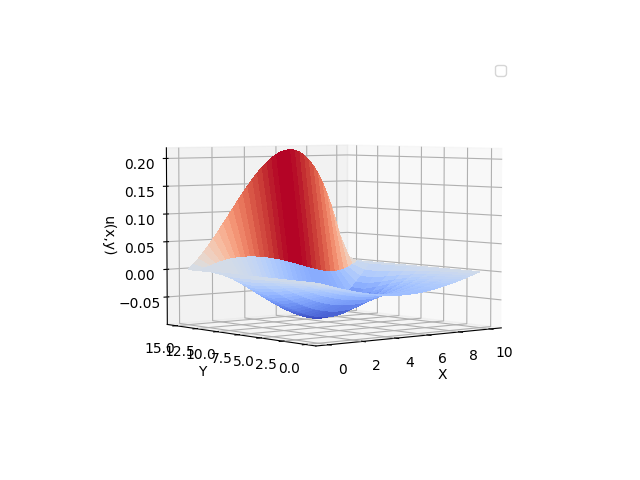
\includegraphics[width=0.49\textwidth, scale=1]{images/results/static_1/function_u_1.png}
        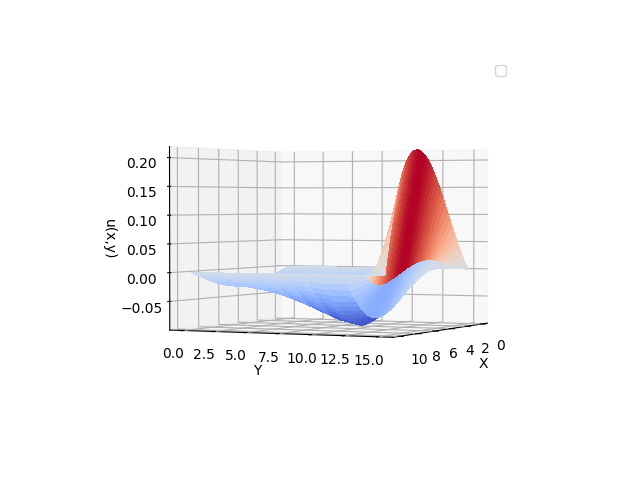
\includegraphics[width=0.49\textwidth, scale=1]{images/results/static_1/function_u_2.png}
        \caption{Функція $u(x, y)$}\label{static_1_u_1}
    \end{center}
\end{figure}
\newpage
\begin{figure}[h!]
    \begin{center}
        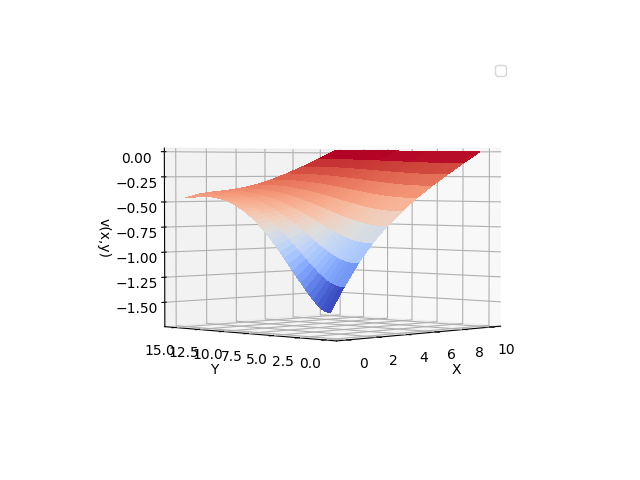
\includegraphics[width=0.49\textwidth, scale=1]{images/results/static_1/function_v_1.png}
        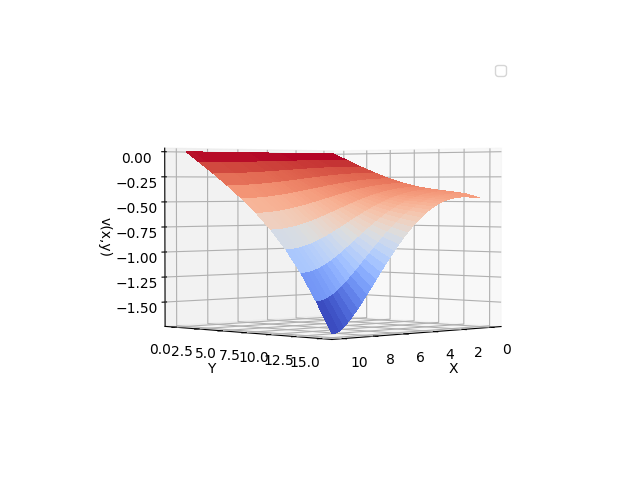
\includegraphics[width=0.49\textwidth, scale=1]{images/results/static_1/function_v_2.png}
        \caption{Функція $v(x, y)$}\label{static_1_v_1}
    \end{center}
\end{figure}
\begin{figure}[h!]
    \begin{center}
        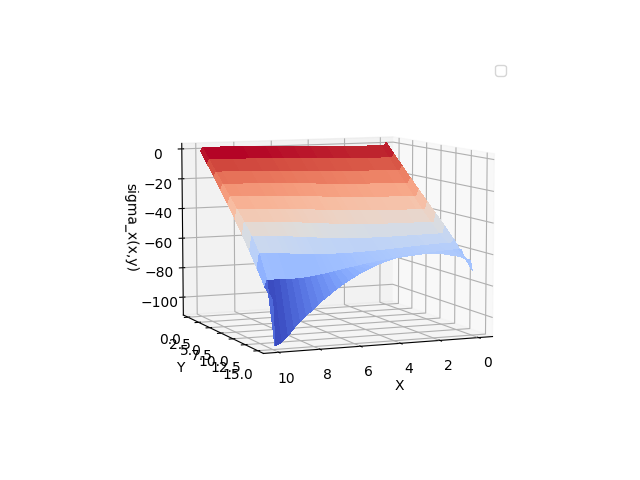
\includegraphics[width=0.49\textwidth, scale=1]{images/results/static_1/function_sigma_x_1.png}
        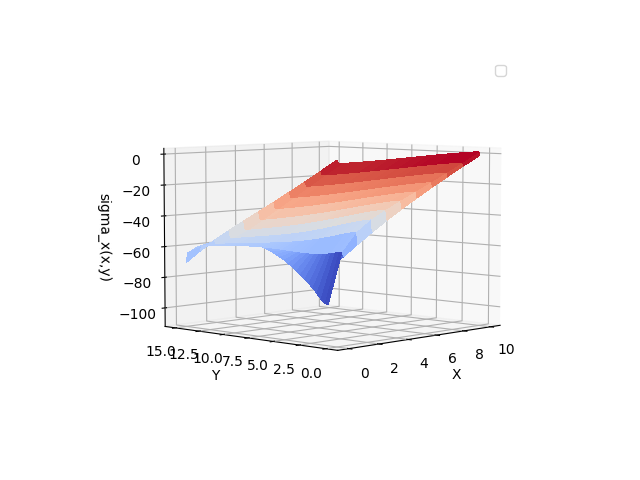
\includegraphics[width=0.49\textwidth, scale=1]{images/results/static_1/function_sigma_x_2.png}
        \caption{Функція $\sigma_x(x, y)$}\label{static_1_sigma_x_1}
    \end{center}
\end{figure}
\begin{figure}[h!]
    \begin{center}
        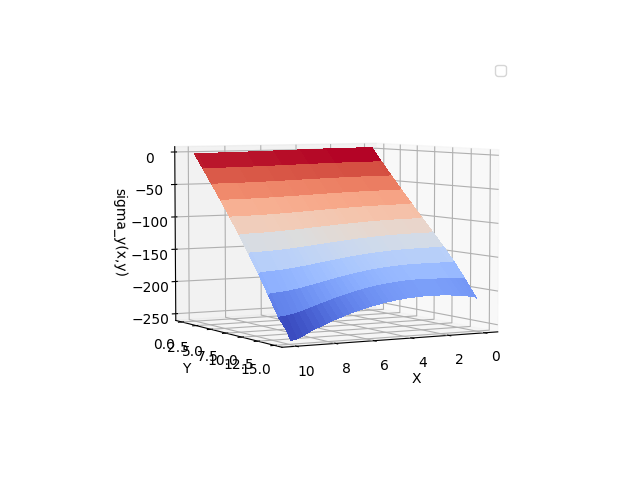
\includegraphics[width=0.49\textwidth, scale=1]{images/results/static_1/function_sigma_y_1.png}
        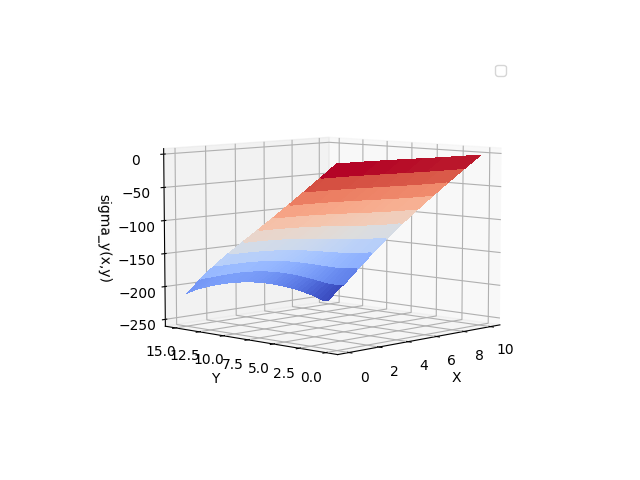
\includegraphics[width=0.49\textwidth, scale=1]{images/results/static_1/function_sigma_y_2.png}
        \caption{Функція $\sigma_y(x, y)$}\label{static_1_sigma_y_1}
    \end{center}
\end{figure}

\subsection{Висновки до треттього розділу розділу}
Отримано точне розв'язок статичної задачі для прямокутної області за умов ідеального контакту на бічних гранях.
Дослідженно поля переміщень та напружень для різних видів навантаження і розмірів прямокутної області.
\subsection{Динамічна задача теорії пружності для прямокутної області за умов ідеального контакту на бічних гранях}
\subsubsection{Постановка задачі}
\begin{figure}[h]
    \begin{center}
        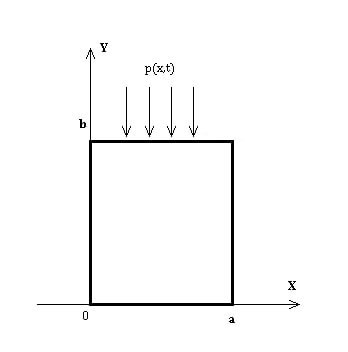
\includegraphics[scale=1]{images/geometry/image_4.jpg}
    \end{center}
    \caption{Геометрія проблеми}\label{geom_dynamic_1}
\end{figure}
Розглядається пружна сама прямокутна область (Рис: \ref{geom_dynamic_1}), яка займає облась,
що описується у декартовій системі координат співвідношенням $0 \le x \le a$, $0 \le y \le b$.

До прямокутної області на грані $y=b$ додане нормальне навантаження
\begin{equation}
    \sigma_y(x, y, t) |_{y=b} = -p(x, t), \quad  \tau_{xy}(x,y,t) |_{y=b} =0
\end{equation}
де $p(x,t)$ відома функція.
На бічних гранях виконується умова ідеального контакту
\begin{equation}
    u(x,y,t) |_{x=0} = 0, \quad \tau_{xy}(x,y,t) |_{x=0} =0
\end{equation}
\begin{equation}
    u(x,y,t) |_{x=a} = 0, \quad \tau_{xy}(x,y,t) |_{x=a} =0
\end{equation}
На нижній грані виконуються наступні умови
\begin{equation}
    v(x,y,t) |_{y=0} = 0, \quad \tau_{xy}(x,y,t) |_{y=0} =0
\end{equation}
Розглядаються наступні рівняння рівноваги Ламе:
\begin{equation}
    \begin{cases}
        \frac{\partial^2 u(x,y,t)}{\partial x^2} + \frac{\partial^2 u(x,y,t)}{\partial y^2} + \mu_0 (\frac{\partial^2 u(x,y,t)}{\partial x^2} + \frac{\partial^2 v(x,y,t)}{\partial x\partial y}) = \frac{1}{c_1^2} \frac{\partial^2 u(x,y,t)}{\partial t^2} \\
        \frac{\partial^2 v(x,y,t)}{\partial x^2} + \frac{\partial^2 v(x,y,t)}{\partial y^2} + \mu_0 (\frac{\partial^2 u(x,y,t)}{\partial x \partial y} + \frac{\partial^2 v(x,y,t)}{\partial y^2}) = \frac{1}{c_2^2} \frac{\partial^2 v(x,y,t)}{\partial t^2} \\
    \end{cases}
\end{equation}

Будемо розглядати випадок гармонічних коливань, тому можемо предствавити функції у наступному вигляді:
\begin{equation}
    u(x,y,t) = u(x,y) e^{i \omega t}, \quad v(x,y,t) = v(x,y) e^{i \omega t}, \quad p(x,t) = p(x) e^{i \omega t}
\end{equation}
Таким чином отримаємо наступні рівняння рівноваги:
\begin{equation}\label{lame_dynamic_1}
    \begin{cases}
        \frac{\partial^2 u(x,y)}{\partial x^2} + \frac{\partial^2 u(x,y)}{\partial y^2} + \mu_0 (\frac{\partial^2 u(x,y)}{\partial x^2} + \frac{\partial^2 v(x,y)}{\partial x\partial y}) = -\frac{\omega^2}{c_1^2}  u(x,y) \\
        \frac{\partial^2 v(x,y)}{\partial x^2} + \frac{\partial^2 v(x,y)}{\partial y^2} + \mu_0 (\frac{\partial^2 u(x,y)}{\partial x \partial y} + \frac{\partial^2 v(x,y)}{\partial y^2}) = -\frac{\omega^2}{c_2^2} v(x,y) \\
    \end{cases}
\end{equation}
Та граничні умови:
\begin{equation}\label{bound_dynamic_1}
    \begin{cases}
        \sigma_y(x, y) |_{y=b} = -p(x, t), \quad  \tau_{xy}(x,y) |_{y=b} = 0 \\
        v(x,y) |_{y=0} = 0, \quad \tau_{xy}(x,y) |_{y=0} = 0 \\
        u(x,y) |_{x=0} = 0, \quad \tau_{xy}(x,y) |_{x=0} = 0 \\
        u(x,y) |_{x=a} = 0, \quad \tau_{xy}(x,y) |_{x=a} = 0 
    \end{cases}
\end{equation}

\subsubsection{Побудова точного розв'язку вихідної задачі}
Для того, щоб звести задачу до одновимірної задачі, використаємо інтегральне перетворення Фур'є по змінній $x$ до рівнянь (\ref{lame_dynamic_1}) наступному вигляді:
\begin{equation}
    \begin{pmatrix}
        u_n(y) \\
        v_n(y)
    \end{pmatrix} = \int_{0}^{a} 
    \begin{pmatrix}
        u(x,y) sin(\alpha_n x) \\
        v(x,y) cos(\alpha_n x)
    \end{pmatrix} dx, \quad \alpha_n = \frac{\pi n}{a}
\end{equation}

Для цього помножимо перше та друге рівняння (\ref{lame_dynamic_1}) на $sin(\alpha_n x)$ та $cos(\alpha_n x)$ відповідно та проінтегруємо по змінній $x$ на інтервалі $0 \le x \le a$.
Покрокове інтегрування рівняння (\ref{lame_dynamic_1}) наведено у (\nameref{ap_A}).
Отримана система рівнянь задачі у просторі трансформант:
\begin{equation}\label{transf_dynamic_1}
    \begin{cases}
        u_n^{''}(y) - \alpha_n \mu_0 v_n^{'}(y) + (-\alpha_n^2 -\alpha_n^2 \mu_0 + \frac{\omega^2}{c_1^2}) u_n(y) = 0 \\
        (1 + \mu_0) v_n^{''}(y) + \alpha_n \mu_0 u_n^{'}(y) + (- \alpha_n^2 + \frac{\omega^2}{c_2^2}) v_n(y) = 0 \\
    \end{cases}
\end{equation}

Застосовуючи інтегральне перетворення до граничних умов,
отримаємо наступні умови задачі у просторі трансформант
\begin{equation}\label{transf_bound_dynamic_1}
    \begin{cases}
        \left( (2G + \lambda)v_n^{'}(y) + \alpha_n \lambda u_n(y) \right)|_{y=b} = -p_n \\
        \left(u_n^{'}(y) - \alpha_n v_n(y)  \right)|_{y=b} = 0 \\
        v_n(y)|_{y=0} = 0 \\
        \left(u_n^{'}(y) - \alpha_n v_n(y)  \right)|_{y=0} = 0
    \end{cases}
\end{equation}
де $p_n = \int_{0}^{a} p(x) cos(\alpha_n x) dx$

Для того щоб розв'язати задачу у простосторі трансформант, перепишмо її у матрично-векторній формі.
Рівняння рівноваги (\ref{transf_dynamic_1}) запишемо у наступному вигляді:
\begin{align}\label{transf_mat_dynamic_1}
    &L_2\left[ Z_n(y) \right] = A * Z_n^{''}(y) + B * Z_n^{'}(y) + C * Z_n(y) \nonumber \\
    &L_2\left[ Z_n(y) \right] = 0
\end{align}
Де
\begin{equation*}
    A = \begin{pmatrix}
        1 & 0 \\
        0 & 1 + \mu_0
    \end{pmatrix}, \quad
    B = \begin{pmatrix}
        0 & -\alpha_n \mu_0 \\
        \alpha_n \mu_0 & 0
    \end{pmatrix}
\end{equation*}
\begin{equation*}
    C = \begin{pmatrix}
        -\alpha_n^2 -\alpha_n^2 \mu_0 + \frac{\omega^2}{c_1^2} & 0 \\
        0 & -\alpha_n^2 + \frac{\omega^2}{c_2^2}
    \end{pmatrix}, \quad
    Z_n(y) = \begin{pmatrix}
        u_n(y) \\
        v_n(y)
    \end{pmatrix}
\end{equation*}
Граничні умови (\ref{transf_bound_dynamic_1}) запишемо у наступному вигляді:
\begin{align}\label{transf_bound_mat_dynamic_1}
    &U_i\left[ Z_n(y) \right] = E_i * Z_n^{'}(b_i) + F_i * Z_n(b_i) \nonumber \\
    & U_i\left[ Z_n(y) \right] = D_i
\end{align}
Де $i = \overline{0, 1}$, $b_0 = b$, $b_1 = 0$,
\begin{equation*}
    E_0 = \begin{pmatrix}
        1 & 0 \\
        0 & 2G + \lambda
    \end{pmatrix}, \quad
    F_0 = \begin{pmatrix}
        0 & -\alpha_n \\
        \alpha_n \lambda & 0
    \end{pmatrix}, \quad
\end{equation*}
\begin{equation*}
    E_1 = \begin{pmatrix}
        1 & 0 \\
        0 & 0
    \end{pmatrix}, \quad
    F_1 = \begin{pmatrix}
        0 & -\alpha_n \\
        0 & 1
    \end{pmatrix}, \quad
\end{equation*}
\begin{equation*}
    D_0 = \begin{pmatrix}
        0 \\
        -p_n
    \end{pmatrix}, \quad
    D_1 = \begin{pmatrix}
        0 \\
        0
    \end{pmatrix}, \quad
\end{equation*}

Для знаходження розв'язку задачі у просторі трансформант, знайдем фундаментальну матрицю рівняння (\ref{transf_mat_dynamic_1}).
Шукати її будем у наступному вигляді \cite{gantmaher}:
\begin{equation}
    Y(y) = \frac{1}{2\pi i} \oint_C e^{sy} M^{-1}(s)ds
\end{equation}
Де $M(s)$ - характерестична матриця рівняння (\ref{transf_mat_dynamic_1}), а $C$ - замкнений контур який містить усі особливі точки. Яку будемо шукати з наступної умовни
\begin{equation}
    L_2\left[ e^{sy}*I \right] = e^{sy} * M(s), \quad I = \begin{pmatrix} 1 & 0 \\ 0 & 1 \end{pmatrix}
\end{equation}
\begin{align*}
    &L_2\left[ e^{sy}*I \right] = e^{sy} \left( s^2A * I + s B*I + C*I \right) = \\
    &=e^{sy} \begin{pmatrix}
        s^2 - \alpha_n^2 - \alpha_n^2\mu_0 + \frac{\omega^2}{c_1^2} & -\alpha_n \mu_0 s \\
        \alpha_n \mu_0 s & s^2 (1 + \mu_0) -\alpha_n^2 + \frac{\omega^2}{c_1^2}
     \end{pmatrix} \Rightarrow
\end{align*}

\begin{equation}
    M(s) = \begin{pmatrix}
        s^2 - \alpha_n^2 - \alpha_n^2\mu_0 + \frac{\omega^2}{c_1^2} & -\alpha_n \mu_0 s \\
        \alpha_n \mu_0 s & s^2 (1 + \mu_0) -\alpha_n^2 + \frac{\omega^2}{c_2^2}
     \end{pmatrix}
\end{equation}

Знайдемо тепер $M^{-1}(s) = \frac{\widetilde{M(s)}}{det[M(s)]}$.
\begin{equation}
    \widetilde{M(s)} = \begin{pmatrix}
        s^2 (1 + \mu_0) -\alpha_n^2 + \frac{\omega^2}{c_2^2} & \alpha_n \mu_0 s \\
        -\alpha_n \mu_0 s & s^2 - \alpha_n^2 - \alpha_n^2\mu_0 + \frac{\omega^2}{c_1^2}
     \end{pmatrix}
\end{equation}
\begin{align}
    &det[M(s)] = \begin{vmatrix}
        s^2 - \alpha_n^2 - \alpha_n^2\mu_0 + \frac{\omega^2}{c_1^2} & -\alpha_n \mu_0 s \\
        \alpha_n \mu_0 s & s^2 (1 + \mu_0) -\alpha_n^2 + \frac{\omega^2}{c_2^2}
     \end{vmatrix} = \nonumber \\
    &=(s - s_1)(s + s_1)(s - s_2)(s + s_2)
\end{align}
Де $s_1$, $s_2$, $-s_1$, $-s_2$ корені $det[M(s)]=0$, детальне знаходження яких наведено в (\nameref{ap_B}).

Враховучи це, тепер знайдемо значення фундаментальної матрицю за допомогою теореми про лишки:
\begin{align*}
    &\frac{1}{2\pi i} \oint_C e^{sy} M^{-1}(s)ds = \frac{2 \pi i}{2 \pi i (1 + \mu_0)} \sum_{i=1}^{4} Res\left[ e^{sy} \frac{\widetilde{M(s)}}{det[M(s)]} \right] = \\
    & = \left(Y_0(y) + Y_1(y) + Y_2(y) + Y_3(y) \right)
\end{align*}
Знайдем $Y_0(y)$:
\begin{align}
    &Y_0(y) =  \left( \frac{e^{sy}}{(s+s_1)(s - s_2)(s + s_2)} \widetilde{M(s)} \right) \Big|_{s=s_1} = \nonumber \\
    &=\frac{e^{s_1 y}}{2s_1 (s_1^2 - s_2^2)} \begin{pmatrix}
        s_1^2 (1 + \mu_0) -\alpha_n^2 + \frac{\omega^2}{c_2^2} & \alpha_n \mu_0 s_1 \\
        -\alpha_n \mu_0 s_1 & s_1^2 - \alpha_n^2 - \alpha_n^2\mu_0 + \frac{\omega^2}{c_1^2}
    \end{pmatrix}
\end{align}
Знайдем $Y_1(y)$:
\begin{align}
    &Y_1(y) =  \left( \frac{e^{sy}}{(s-s_1)(s - s_2)(s + s_2)} \widetilde{M(s)} \right) \Big|_{s=-s_1} = \nonumber \\
    &=-\frac{e^{-s_1 y}}{2s_1 (s_1^2 - s_2^2)} \begin{pmatrix}
        s_1^2 (1 + \mu_0) -\alpha_n^2 + \frac{\omega^2}{c_2^2} & -\alpha_n \mu_0 s_1 \\
        \alpha_n \mu_0 s_1 & s_1^2 - \alpha_n^2 - \alpha_n^2\mu_0 + \frac{\omega^2}{c_1^2}
    \end{pmatrix}
\end{align}
Знайдем $Y_2(y)$:
\begin{align}
    &Y_2(y) =  \left( \frac{e^{sy}}{(s+s_2)(s - s_1)(s + s_1)} \widetilde{M(s)} \right) \Big|_{s=s_2} = \nonumber \\
    &=\frac{e^{s_2 y}}{2s_2 (s_2^2 - s_1^2)} \begin{pmatrix}
        s_2^2 (1 + \mu_0) -\alpha_n^2 + \frac{\omega^2}{c_2^2} & \alpha_n \mu_0 s_2 \\
        -\alpha_n \mu_0 s_2 & s_2^2 - \alpha_n^2 - \alpha_n^2\mu_0 + \frac{\omega^2}{c_1^2}
    \end{pmatrix}
\end{align}
Знайдем $Y_3(y)$:
\begin{align}
    &Y_3(y) =  \left( \frac{e^{sy}}{(s-s_2)(s - s_1)(s + s_1)} \widetilde{M(s)} \right) \Big|_{s=-s_2} = \nonumber \\
    &=-\frac{e^{-s_2 y}}{2s_2 (s_2^2 - s_1^2)} \begin{pmatrix}
        s_2^2 (1 + \mu_0) -\alpha_n^2 + \frac{\omega^2}{c_2^2} & -\alpha_n \mu_0 s_2 \\
        \alpha_n \mu_0 s_2 & s_2^2 - \alpha_n^2 - \alpha_n^2\mu_0 + \frac{\omega^2}{c_1^2}
    \end{pmatrix}
\end{align}

Таким чином ми можемо записати розв'язок задачі у просторі трансформант:
\begin{equation}
    Z_n(y) =\left( Y_0(y) +  Y_1(y)  \right) * \begin{pmatrix} c_1 \\ c_2 \end{pmatrix} + \left( Y_2(y) +  Y_3(y) \right) * \begin{pmatrix} c_3 \\ c_4 \end{pmatrix}
\end{equation}
Залишилось знайти невідомі коєфіцієнти $c_1$, $c_2$, $c_3$, $c_4$, використовуючи граничні умови (\ref{transf_bound_mat_dynamic_1}).
Покрокове знаходження коєфіцієнтів наведено у (\nameref{ap_E}).
Таким чином ми можемо записати розв'зок у просторі трансформант:
\begin{align}\label{transf_sol_u_dynamic_1}
    &u_n(y) = \frac{( s_1^2 (1 + \mu_0) -\alpha_n^2 + \frac{\omega^2}{c_2^2})(e^{s_1y} - e^{-s_1y})}{2s_1(s_1^2 - s_2^2)(1 + \mu_0)}c_1 + \nonumber \\
    & + \frac{( s_2^2 (1 + \mu_0) -\alpha_n^2 + \frac{\omega^2}{c_2^2})(e^{s_2y} - e^{-s_2y})}{2s_2(s_2^2 - s_1^2)(1 + \mu_0)}c_3 + \nonumber \\
    & + \frac{( s_1 \alpha_n y)(e^{s_1y} + e^{-s_1y})}{2s_1(s_1^2 - s_2^2)(1 + \mu_0)}c_2 + \frac{(s_2 \alpha_n y)(e^{s_2y} + e^{-s_2y})}{2s_2(s_2^2 - s_1^2)(1 + \mu_0)}c_4
\end{align}
\begin{align}\label{transf_sol_v_dynamic_1}
    &v_n(y) = \frac{(s_1^2 - \alpha_n^2 - \alpha_n^2\mu_0 + \frac{\omega^2}{c_1^2})(e^{s_1y} - e^{-s_1y})}{2s_1(s_1^2 - s_2^2)(1 + \mu_0)}c_2 + \nonumber \\
    & +\frac{(s_2^2 - \alpha_n^2 - \alpha_n^2\mu_0 + \frac{\omega^2}{c_1^2})(e^{s_2y} - e^{-s_2y})}{2s_2(s_2^2 - s_1^2)(1 + \mu_0)}c_4 - \nonumber \\
    & - \frac{(s_1 \alpha_n y)(e^{s_1y} + e^{-s_1y})}{2s_1(s_1^2 - s_2^2)(1 + \mu_0)}c_1 - \frac{(s_2 \alpha_n y)(e^{s_2y} + e^{-s_2y})}{2s_2(s_2^2 - s_1^2)(1 + \mu_0)}c_3
\end{align}

Викорустовуючи обернене інтегральне перетворення Фур'є до розв'язку задачі у просторі трансформант
(\ref{transf_sol_u_dynamic_1}), (\ref{transf_sol_v_dynamic_1}), отримаємо фінальний розв'язок задачі
\begin{equation}
    u(x,y) = \frac{2}{a} \sum_{n=1}^{\infty} u_n(y) sin(\alpha_n x), \quad \alpha_n = \frac{\pi n}{a}
\end{equation}
\begin{equation}
    v(x,y) = \frac{v_0(y)}{a} + \frac{2}{a} \sum_{n=1}^{\infty} v_n(y) cos(\alpha_n x), \quad \alpha_n = \frac{\pi n}{a}
\end{equation}

Останній крок це знаходження $v_0(y)$ у випадку коли $n=0$, $\alpha_n =0$.
Для цього повернемся до другого рівняння (\ref{transf_dynamic_1}), та запишем його для цього випадку:
\begin{equation}\label{transf_v_0_dynamic_1}
    (1 + \mu_0) v_n^{''}(y) + \frac{\omega^2}{c_2^2}v_0(y) = 0
\end{equation}
Та граничні умови:
\begin{equation}\label{transf_bound_v_0_dynamic_1}
    \begin{cases}
        (2G + \lambda)v_0^{'}(y)|_{y=b} = -p_0 \\
        v_0(y)|_{y=0} = 0
    \end{cases}
\end{equation}
Де $p_0 = \int_{0}^{a}p(x)dx$

Розв'язок рівняння (\ref{transf_v_0_dynamic_1}):
\begin{equation}
    v_0(y) = c_1 cos \left(y \sqrt{\frac{\omega^2}{c_2^2(1 + \mu_0)}} \right) + c_2 sin \left( y \sqrt{\frac{\omega^2}{c_2^2(1 + \mu_0)}} \right)
\end{equation}
Застовоючи граничні умови (\ref{transf_bound_v_0_dynamic_1}) для знаходження коєфіцієнтів $c_1$, $c_2$, отримаємо розв'язок задачі задачі:
\begin{equation}
    v_0(y) = \frac{-p_0}{(2G + \lambda) \sqrt{\frac{\omega^2}{c_2^2(1 + \mu_0)}} sin \left(b \sqrt{\frac{\omega^2}{c_2^2(1 + \mu_0)}} \right) } sin \left(y \sqrt{\frac{\omega^2}{c_2^2(1 + \mu_0)}} \right)
\end{equation}

\subsubsection{Чисельні розрахунки}
Наведені чисельні експеренти розглядаються для сталі ($E=200$ ГПА, $\mu=0.25$).

Розглянута прямокунта область $0 \le x \le 10$, $0 \le y \le 15$, при функції навантаження $p(x)=(x-2.5)^2$ та частоті коливань $\omega=0.75$.
На малюнках (Рис: \ref{static_1_u_1}), (Рис: \ref{static_1_v_1}), (Рис: \ref{static_1_sigma_x_1}), (Рис: \ref{static_1_sigma_y_1})
представлені функіі переміщень $u(x,y)$, $v(x,y)$ та напружень $\sigma_x(x,y)$, $\sigma_y(x,y)$ відповідно.


\subsection{Висновки до третього розділу}
Отримано точне розв'язок статичної та динамічної задачі для прямокутної області за умов ідеального контакту на бічних гранях.
Дослідженно поля переміщень та напружень для різних видів навантаження і розмірів прямокутної області.
\newpage

\section[МІШАНА ЗАДАЧА ДЛЯ ПРЯМОКУТНОЇ ОБЛАСТІ ЗА УМОВ ДРУГОЇ ОСНОВНОЇ ЗАДАЧІ ТЕОРІЇ ПРУЖНОСТІ НА БІЧНИХ ГРАНЯХ]
{\centering МІШАНА ЗАДАЧА ДЛЯ ПРЯМОКУТНОЇ ОБЛАСТІ ЗА УМОВ ДРУГОЇ ОСНОВНОЇ ЗАДАЧІ ТЕОРІЇ ПРУЖНОСТІ НА БІЧНИХ ГРАНЯХ}
У даному розділі досліджено плоскі статична та динамічна задачі теорії пружності для прямокутної області,
за умов другої основної задачі теорії пружності на бічних гранях.

Вихідні задачі зведено до одновимірної задачі у просторі трансформант за допомогою інтегрального перетворення Фур'є.
Розв'зок одновимірної задачі у просторі трансформант знайдено як суперпозиція загального розв'язку векторного однорідного рівняння
та часткового розв'язку неоднорідного рівняння.
Загальний розв'язок векторного однорідного рівняння знайдено за допомогою методу матричного диференціального числення.
Частковий розв'язок неоднорідного рівняння знайдено за допомогою матричної функції Гріна.
Остаточне подання для полів переміщень та напружень наведено за допомогою оберненного перетворення Фур'є.

Проведено чисельний аналіз отриманих функцій переміщень та напружень для різних розмірів прямокутної області та різних видів навантаження.

Результати розділу опубліковані в \cite{pozhylenkov_4}, \cite{pozhylenkov_6}, а також доповідалась на конференції \cite{conf_3}, \cite{conf_5}.
\subsection{Статична задача для прямокутної області за умов другої основної задачі теорії пружності на бічних гранях}
У даному розділі досліджено плоска статична задача теорії пружності для прямокутної області,
за умов другої основної задачі теорії пружності на бічних гранях.

Вихідна задача зведена до одновимірної задачі у просторі трансформант за допомогою інтегрального перетворення Фур'є.
Отримана крайова задача розв'язана точно за допомогою методу матрично диференціального числення,
фундаментальний розв'язок представлений як інтеграл по замкненому контору, який в свою чергу, був знайденний за допомогою теоремі про лишки.
Остаточний вигляд для функцій переміщеннь та напружень отриман шляхом оберненого перетворення Фур'є.
Побудовано та розв'язано сінгульрне інтегральне рівняння відносно невідомої функції шляхом викорстання методу ортагональних поліномів, та зведення рівнняння до бескінечної алгебричної системи,
яка в подальшому була розв'язана методом редукціі.

Проведено чисельний аналіз отриманих функцій переміщень та напружень для різних розмірів прямокутної області та різних видів навантаження.

\subsection{Постановка задачі}
\begin{figure}[ht!]
    \begin{center}
        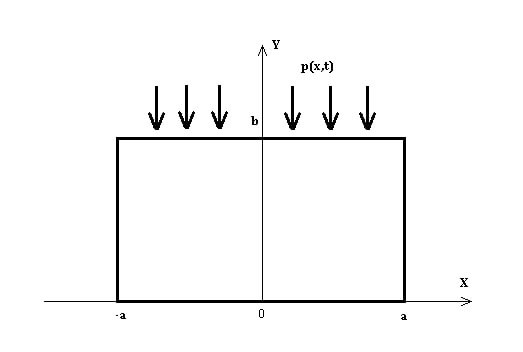
\includegraphics[scale=1]{images/geometry/image_1.jpg}
    \end{center}
    \caption{Геометрія проблеми}\label{geom_static_2}
\end{figure}
Розглядається пружна прямокутна область (Рис: \ref{geom_static_2}), яка займає облась,
що описується у декартовій системі координат співвідношенням $-a \le x \le a$, $0 \le y \le b$.

До прямокутної області на грані $y=b$ додане нормальне навантаження
\begin{equation}
    \sigma_y(x, y) |_{y=b} = -p(x), \quad  \tau_{xy}(x,y) |_{y=b} =0
\end{equation}
де $p(x)$ відома функція.

На бічних гранях виконується умова другої основної задачі теорії пружності
\begin{equation}
    u(x,y) |_{x=\pm a} = 0, \quad v(x,y) |_{x=\pm a} =0
\end{equation}
На нижній грані виконуються наступні умови
\begin{equation}
    v(x,y) |_{y=0} = 0, \quad \tau_{xy}(x,y) |_{y=0} =0
\end{equation}
Розглядаються наступні рівняння рівноваги Ламе:
\begin{equation}\label{lame_static_2}
    \begin{cases}
        \frac{\partial^2 u(x,y)}{\partial x^2} + \frac{\partial^2 u(x,y)}{\partial y^2} + \mu_0 (\frac{\partial^2 u(x,y)}{\partial x^2} + \frac{\partial^2 v(x,y)}{\partial x\partial y}) = 0 \\
        \frac{\partial^2 v(x,y)}{\partial x^2} + \frac{\partial^2 v(x,y)}{\partial y^2} + \mu_0 (\frac{\partial^2 u(x,y)}{\partial x \partial y} + \frac{\partial^2 v(x,y)}{\partial y^2}) = 0 \\
    \end{cases}
\end{equation}
Щоб розв'язати поставлену задачу буде розглянута тільки половона прямокутної області $0 \le x \le a$, $0 \le y \le b$
та використовуючи властивості симметрії граничні умови на бічних гранях будуть мати вигляд:
\begin{equation}\label{bound_1_static_2}
    u(x,y) |_{x=0} = 0, \quad \tau_{xy}(x,y) |_{x=0} =0
\end{equation}
\begin{equation}\label{bound_2_static_2}
    u(x,y) |_{x=a} = 0, \quad v(x,y) |_{x=a} = 0
\end{equation}

\subsection{Зведеня задачі до одновимірної у просторі трансформант}
Для того, щоб звести задачу до одновимірної задачі, використаєм інтегральне перетворення Фур'є по змінній $x$ у до рівнянь (\ref{lame_static_2}) наступному вигляді:
\begin{equation}
    \begin{pmatrix}
        u_n(y) \\
        v_n(y)
    \end{pmatrix} = \int_{0}^{a} 
    \begin{pmatrix}
        u(x,y) sin(\alpha_n x) \\
        v(x,y) cos(\alpha_n x)
    \end{pmatrix} dx, \quad \alpha_n = \frac{\pi n}{a}
\end{equation}

Для цього помножим перше та друге рівняння (\ref{lame_static_2}) на $sin(\alpha_n x)$ та $cos(\alpha_n x)$ відповідно та проінтегруєм по змінній $x$ на інтервалі $0 \le x \le a$.
Покрокове інтегрування рівняння (\ref{lame_static_2}) наведено у (\nameref{ap_A}).
Отримана система рівнянь задачі у просторі трансформант:
\begin{equation}\label{transf_static_2}
    \begin{cases}
        u_n^{''}(y) - \alpha_n \mu_0 v_n^{'}(y) - \alpha_n^2 (1 + \mu_0) u_n(y) = 0 \\
        (1 + \mu_0) v_n^{''}(y) + \alpha_n \mu_0 u_n^{'}(y)  - \alpha_n^2 v_n(y) = -cos(\alpha_n) \frac{\partial v(x,y)}{\partial x}|_{x=a} \\
    \end{cases}
\end{equation}
\subsection{Динамічна задача для прямокутної області за умов другої основної задачі теорії пружності на бічних гранях}
У даному розділі досліджено плоска динамічна задача теорії пружності для прямокутної області,
за другої основної задачі теорії пружності на бічних гранях.

Вихідна задача зведена до одновимірної задачі у просторі трансформант за допомогою інтегрального перетворення Фур'є.
Отримана крайова задача розв'язана точно за допомогою методу матрично диференціального числення,
фундаментальний розв'язок представлений як інтеграл по замкненому контору, який в свою чергу, був знайденний за допомогою теоремі про лишки.
Побудована матриця-функція Гріна як комбінація фундаментальних базисних розв'язків задачі у просторі трансформант.
Остаточний вигляд для функцій переміщеннь та напружень отриман шляхом оберненого перетворення Фур'є.
Побудовано та розв'язано сінгульрне інтегральне рівняння відносно невідомої функції шляхом викорстання методу ортагональних многочленів, та зведення рівнняння до бескінечної алгебричної системи,
яка в подальшому була розв'язана методом редукціі \cite{popov_3}.

Проведено чисельний аналіз отриманих функцій переміщень та напружень для різних розмірів прямокутної області та різних видів навантаження.

\subsection{Постановка задачі}
\begin{figure}[h]
    \begin{center}
        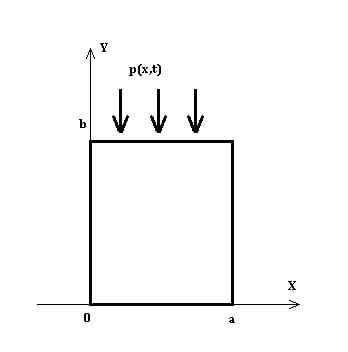
\includegraphics[scale=1]{images/geometry/image_2.jpg}
    \end{center}
    \caption{Геометрія проблеми}\label{geom_dynamic_2}
\end{figure}
Розглядається пружна сама прямокутна область (Рис: \ref{geom_dynamic_1}), яка займає облась,
що описується у декартовій системі координат співвідношенням $0 \le x \le a$, $0 \le y \le b$.

До прямокутної області на грані $y=b$ додане нормальне навантаження
\begin{equation}
    \sigma_y(x, y, t) |_{y=b} = -p(x, t), \quad  \tau_{xy}(x,y,t) |_{y=b} =0
\end{equation}
де $p(x,t)$ відома функція.
На бічних гранях виконується умова другої основної задачі теорії пружності
\begin{equation}
    u(x,y,t) |_{x=\pm a} = 0, \quad v(x,y,t) |_{x=\pm a} =0
\end{equation}
На нижній грані виконуються наступні умови
\begin{equation}
    v(x,y,t) |_{y=0} = 0, \quad \tau_{xy}(x,y,t) |_{y=0} =0
\end{equation}
Розглядаються наступні рівняння рівноваги Ламе:
\begin{equation}
    \begin{cases}
        \frac{\partial^2 u(x,y,t)}{\partial x^2} + \frac{\partial^2 u(x,y,t)}{\partial y^2} + \mu_0 (\frac{\partial^2 u(x,y,t)}{\partial x^2} + \frac{\partial^2 v(x,y,t)}{\partial x\partial y}) = \frac{1}{c_1^2} \frac{\partial^2 u(x,y,t)}{\partial t^2} \\
        \frac{\partial^2 v(x,y,t)}{\partial x^2} + \frac{\partial^2 v(x,y,t)}{\partial y^2} + \mu_0 (\frac{\partial^2 u(x,y,t)}{\partial x \partial y} + \frac{\partial^2 v(x,y,t)}{\partial y^2}) = \frac{1}{c_2^2} \frac{\partial^2 v(x,y,t)}{\partial t^2} \\
    \end{cases}
\end{equation}

Будемо розглядати випадок гармонічних коливань, тому можемо предствавити функції у наступному вигляді:
\begin{equation}
    u(x,y,t) = u(x,y) e^{i \omega t}, \quad v(x,y,t) = v(x,y) e^{i \omega t}, \quad p(x,t) = p(x) e^{i \omega t}
\end{equation}
Таким чином отримаємо наступні рівняння рівноваги:
\begin{equation}\label{lame_dynamic_2}
    \begin{cases}
        \frac{\partial^2 u(x,y)}{\partial x^2} + \frac{\partial^2 u(x,y)}{\partial y^2} + \mu_0 (\frac{\partial^2 u(x,y)}{\partial x^2} + \frac{\partial^2 v(x,y)}{\partial x\partial y}) = -\frac{\omega^2}{c_1^2}  u(x,y) \\
        \frac{\partial^2 v(x,y)}{\partial x^2} + \frac{\partial^2 v(x,y)}{\partial y^2} + \mu_0 (\frac{\partial^2 u(x,y)}{\partial x \partial y} + \frac{\partial^2 v(x,y)}{\partial y^2}) = -\frac{\omega^2}{c_2^2} v(x,y) \\
    \end{cases}
\end{equation}
Також, щоб розв'язати поставлену задачу буде розглянута тільки половона прямокутної області $0 \le x \le a$, $0 \le y \le b$
та використовуючи властивості симметрії граничні умови в результаті будуть мати вигляд:
\begin{equation}\label{bound_dynamic_2}
    \begin{cases}
        \sigma_y(x, y) |_{y=b} = -p(x, t), \quad  \tau_{xy}(x,y) |_{y=b} =0 \\
        v(x,y) |_{y=0} = 0, \quad \tau_{xy}(x,y) |_{y=0} = 0 \\
        u(x,y) |_{x=0} = 0, \quad \tau_{xy}(x,y) |_{x=0} = 0 \\
        u(x,y) |_{x=a} = 0, \quad v(x,y) |_{x=a} = 0
    \end{cases}
\end{equation}

\subsection{Зведеня задачі до одновимірної у просторі трансформант}
Для того, щоб звести задачу до одновимірної задачі, використаєм інтегральне перетворення Фур'є по змінній $x$ у до рівнянь (\ref{lame_dynamic_2}) наступному вигляді:
\begin{equation}
    \begin{pmatrix}
        u_n(y) \\
        v_n(y)
    \end{pmatrix} = \int_{0}^{a} 
    \begin{pmatrix}
        u(x,y) sin(\alpha_n x) \\
        v(x,y) cos(\alpha_n x)
    \end{pmatrix} dx, \quad \alpha_n = \frac{\pi n}{a}
\end{equation}

Для цього помножим перше та друге рівняння (\ref{lame_dynamic_2}) на $sin(\alpha_n x)$ та $cos(\alpha_n x)$ відповідно та проінтегруєм по змінній $x$ на інтервалі $0 \le x \le a$.
Покрокове інтегрування рівняння (\ref{lame_dynamic_2}) наведено у (\nameref{ap_A}).
Отримана система рівнянь задачі у просторі трансформант:
\begin{equation}\label{transf_dynamic_2}
    \begin{cases}
        u_n^{''}(y) - \alpha_n \mu_0 v_n^{'}(y) + (-\alpha_n^2 -\alpha_n^2 \mu_0 + \frac{\omega^2}{c_1^2}) u_n(y) = 0 \\
        (1 + \mu_0) v_n^{''}(y) + \alpha_n \mu_0 u_n^{'}(y) + (- \alpha_n^2 + \frac{\omega^2}{c_2^2}) v_n(y) = -cos(\alpha_n) f(y)\\
    \end{cases}
\end{equation}
Де $f(y) = \frac{\partial v(x,y)}{\partial x}|_{x=a}$ - невідома функція

Застосовуючи інтегральне перетворення до граничних умов,
отримаємо наступні умови задачі у просторі трансформант
\begin{equation}\label{transf_bound_dynamic_2}
    \begin{cases}
        \left( (2G + \lambda)v_n^{'}(y) + \alpha_n \lambda u_n(y) \right)|_{y=b} = -p_n \\
        \left(u_n^{'}(y) - \alpha_n v_n(y)  \right)|_{y=b} = 0 \\
        v_n(y)|_{y=0} = 0 \\
        \left(u_n^{'}(y) - \alpha_n v_n(y)  \right)|_{y=0} = 0
    \end{cases}
\end{equation}
Де $p_n = \int_{0}^{a} p(x) cos(\alpha_n x) dx$

\subsection{Зведення задачі у просторі трансформант до матрично-векторної форми}
Для того щоб розв'язати задачу у простосторі трансформант, перепишмо її у матрично-векторній формі.
Рівняння рівноваги (\ref{transf_dynamic_2}) запишемо у наступному вигляді:
\begin{align}\label{transf_mat_dynamic_2}
    &L_2\left[ Z_n(y) \right] = A * Z_n^{''}(y) + B * Z_n^{'}(y) + C * Z_n(y) \nonumber \\
    &L_2\left[ Z_n(y) \right] = F_n(y)
\end{align}
Де
\begin{equation*}
    A = \begin{pmatrix}
        1 & 0 \\
        0 & 1 + \mu_0
    \end{pmatrix}, \quad
    B = \begin{pmatrix}
        0 & -\alpha_n \mu_0 \\
        \alpha_n \mu_0 & 0
    \end{pmatrix},
\end{equation*}
\begin{equation*}
    \centering
    C = \begin{pmatrix}
        -\alpha_n^2 -\alpha_n^2 \mu_0 + \frac{\omega^2}{c_1^2} & 0 \\
        0 & -\alpha_n^2 + \frac{\omega^2}{c_2^2}
    \end{pmatrix},
\end{equation*}
\begin{equation*}
    Z_n(y) = \begin{pmatrix}
        u_n(y) \\
        v_n(y)
    \end{pmatrix}, \quad 
    F_n(y) = \begin{pmatrix}
        0 \\
        - cos(\alpha_n a) f(y)
    \end{pmatrix}
\end{equation*}
Граничні умови (\ref{transf_bound_dynamic_2}) запишемо у наступному вигляді:
\begin{align}\label{transf_bound_mat_dynamic_2}
    &U_i\left[ Z_n(y) \right] = E_i * Z_n^{'}(b_i) + F_i * Z_n(b_i) \nonumber \\
    & U_i\left[ Z_n(y) \right] = D_i
\end{align}
Де $i = \overline{0, 1}$, $b_0 = b$, $b_1 = 0$,
\begin{equation*}
    E_0 = \begin{pmatrix}
        1 & 0 \\
        0 & 2G + \lambda
    \end{pmatrix}, \quad
    F_0 = \begin{pmatrix}
        0 & -\alpha_n \\
        \alpha_n \lambda & 0
    \end{pmatrix}, \quad
\end{equation*}
\begin{equation*}
    E_1 = \begin{pmatrix}
        1 & 0 \\
        0 & 0
    \end{pmatrix}, \quad
    F_1 = \begin{pmatrix}
        0 & -\alpha_n \\
        0 & 1
    \end{pmatrix}, \quad
\end{equation*}
\begin{equation*}
    D_0 = \begin{pmatrix}
        0 \\
        -p_n
    \end{pmatrix}, \quad
    D_1 = \begin{pmatrix}
        0 \\
        0
    \end{pmatrix}, \quad
\end{equation*}

Для знаходження розв'язку задачі у просторі трансформант, знайдем фундаментальну матрицю рівняння (\ref{transf_mat_dynamic_2}).
Шукати її будем у наступному вигляді \cite{gantmaher}:
\begin{equation}
    Y(y) = \frac{1}{2\pi i} \oint_C e^{sy} M^{-1}(s)ds
\end{equation}
Де $M(s)$ - характерестична матриця рівняння (\ref{transf_mat_dynamic_2}), а $C$ - замкнений контур який містить усі особливі точки. Яку будемо шукати з наступної умовни
\begin{equation}
    L_2\left[ e^{sy}*I \right] = e^{sy} * M(s), \quad I = \begin{pmatrix} 1 & 0 \\ 0 & 1 \end{pmatrix}
\end{equation}
\begin{align*}
    &L_2\left[ e^{sy}*I \right] = e^{sy} \left( s^2A * I + s B*I + C*I \right) = \\
    &=e^{sy} \begin{pmatrix}
        s^2 - \alpha_n^2 - \alpha_n^2\mu_0 + \frac{\omega^2}{c_1^2} & -\alpha_n \mu_0 s \\
        \alpha_n \mu_0 s & s^2 (1 + \mu_0) -\alpha_n^2 + \frac{\omega^2}{c_1^2}
     \end{pmatrix} \Rightarrow
\end{align*}

\begin{equation}
    M(s) = \begin{pmatrix}
        s^2 - \alpha_n^2 - \alpha_n^2\mu_0 + \frac{\omega^2}{c_1^2} & -\alpha_n \mu_0 s \\
        \alpha_n \mu_0 s & s^2 (1 + \mu_0) -\alpha_n^2 + \frac{\omega^2}{c_2^2}
     \end{pmatrix}
\end{equation}

Знайдемо тепер $M^{-1}(s) = \frac{\widetilde{M(s)}}{det[M(s)]}$.
\begin{equation}
    \widetilde{M(s)} = \begin{pmatrix}
        s^2 (1 + \mu_0) -\alpha_n^2 + \frac{\omega^2}{c_2^2} & \alpha_n \mu_0 s \\
        -\alpha_n \mu_0 s & s^2 - \alpha_n^2 - \alpha_n^2\mu_0 + \frac{\omega^2}{c_1^2}
     \end{pmatrix}
\end{equation}
\begin{align}
    &det[M(s)] = \begin{vmatrix}
        s^2 - \alpha_n^2 - \alpha_n^2\mu_0 + \frac{\omega^2}{c_1^2} & -\alpha_n \mu_0 s \\
        \alpha_n \mu_0 s & s^2 (1 + \mu_0) -\alpha_n^2 + \frac{\omega^2}{c_2^2}
     \end{vmatrix} = \nonumber \\
    &=(s - s_1)(s + s_1)(s - s_2)(s + s_2)
\end{align}
Де $s_1$, $s_2$, $-s_1$, $-s_2$ корені $det[M(s)]=0$, детальне знаходження яких наведено в (\nameref{ap_B}).

\subsection{Висновки до четвертого розділу розділу}
Отримано точне розв'язок статичної та динамічної задачі для прямокутної області за умов другої основної задачі теорії пружності на бічних гранях.
Дослідженно поля переміщень та напружень для різних видів навантаження і розмірів прямокутної області.
\newpage

\section[ЧИСЛОВІ РОЗРАХУНКИ ТА ЇХ АНАЛІЗ]
{\centering ЧИСЛОВІ РОЗРАХУНКИ ТА ЇХ АНАЛІЗ}
У цьому розіділі наведено числові результати та їх аналіз для задач,
які розв'язано у попередніх розділах.
Усі подальщі розрахунки проведено для для сталі ($E=200$ ГПА, $\mu=0.25$) та зафіксовані розміри прямокутника по осі $y$, $0 \le y \le 15$.
В подальшому для того, щоби розглянути залежності від геометрії тіла,
розмір області буде змінюватись по осі $x$.

\subsection{Статичні задачі}

У цьому пункті проаналізовано статичні задачі теорії пружності для прямокутної області за різних умов на бічних гранях.
Спочатку розлянемо випадок задачі за умов ідеального контакту на бічних гранях,
розв'зок якої наведено у Підрозділі 3.1, та заданної функції навантаження $p(x) = (x - 5.5)^2$.
\begin{figure}[h!]
    \begin{center}
        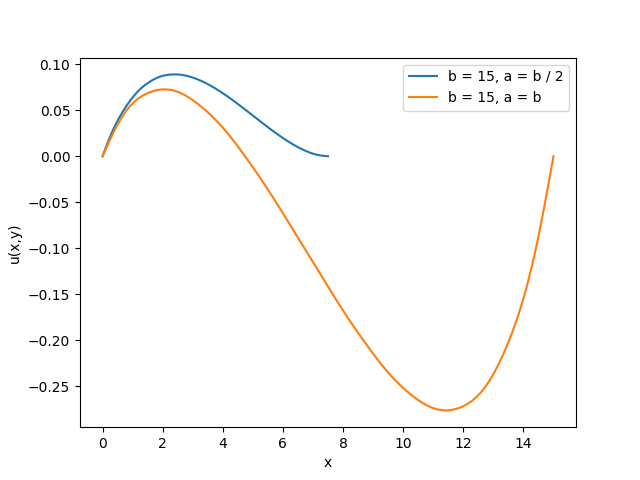
\includegraphics[width=0.49\textwidth, scale=1]{images/results/static_1/u(x,b)1.png}
        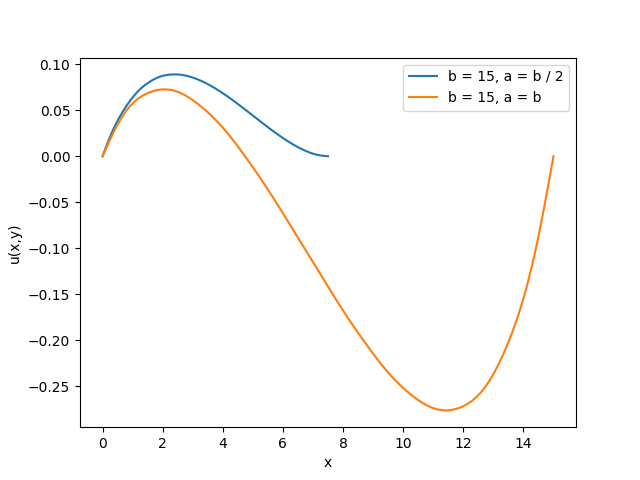
\includegraphics[width=0.49\textwidth, scale=1]{images/results/static_1/u(x,b)2.png}
        \caption{Переміщення $u(x, b)$}\label{static_1_u(x,b)}
    \end{center}
\end{figure}

На Рис. \ref{static_1_u(x,b)} зображено функція переміщеня $u(x, y)$ при $y=b$.
З графіків видно виконання граничних умов на бічних гранях $u(x,y) |_{x=0} = 0$, $u(x,y) |_{x=a} = 0$,
що підтверджує коректність знайденого розв'язку.
Також можна побачити, що при різних розмірах прямокутної області міняється максимальне та мінальне значення функції пермешінення,
при $a = 2b$ мінімум функції набуває найменьшого значення, а для випадку $a = b / 2$ максимум функції набуває найбільшого значення.

\begin{figure}[h!]
    \begin{center}
        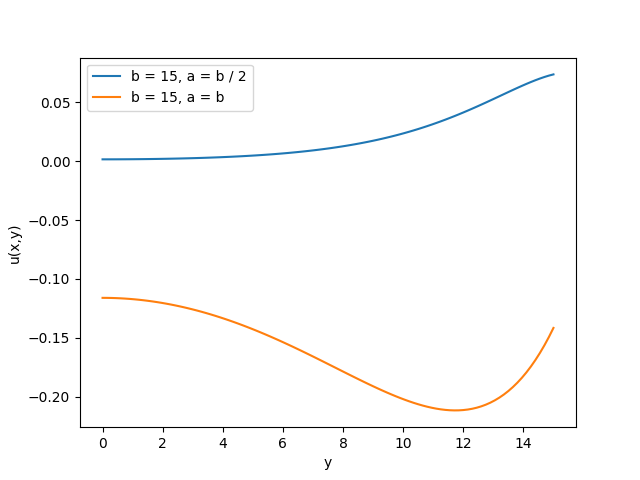
\includegraphics[width=0.49\textwidth, scale=1]{images/results/static_1/u(a:2,y)1.png}
        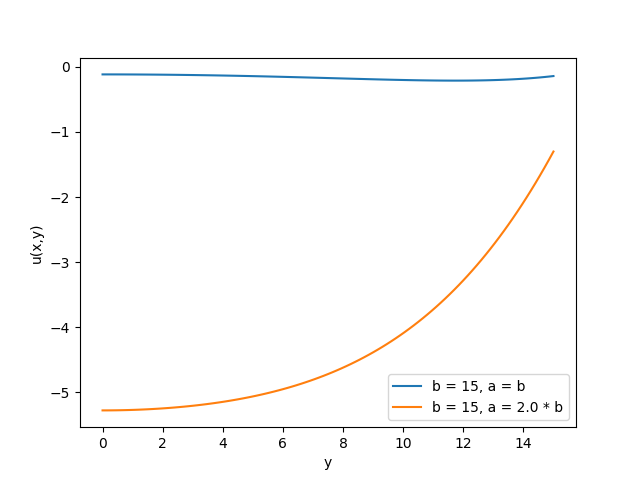
\includegraphics[width=0.49\textwidth, scale=1]{images/results/static_1/u(a:2,y)2.png}
        \caption{Переміщення $u(a/2, y)$}\label{static_1_u(a:2,y)}
    \end{center}
\end{figure}
\begin{figure}[h!]
    \begin{center}
        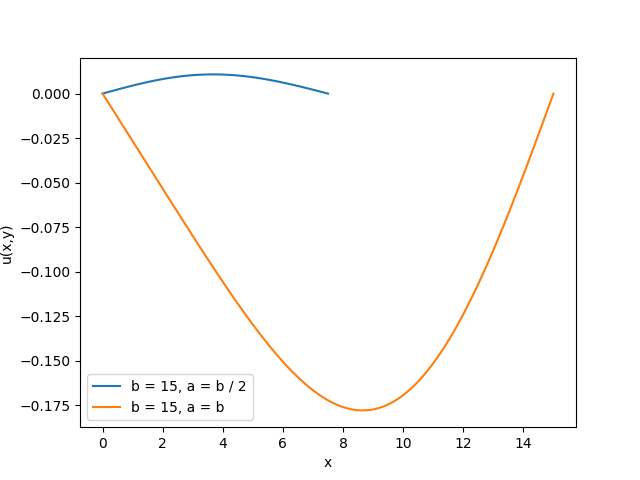
\includegraphics[width=0.49\textwidth, scale=1]{images/results/static_1/u(x,b:2)1.png}
        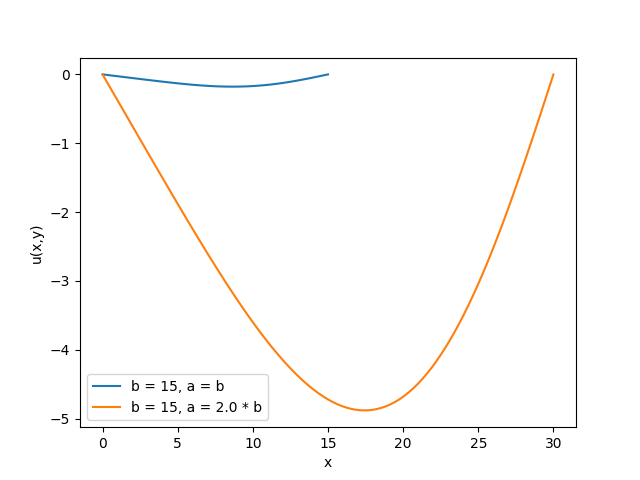
\includegraphics[width=0.49\textwidth, scale=1]{images/results/static_1/u(x,b:2)2.png}
        \caption{Переміщення $u(x, b:2)$}\label{static_1_u(x,b:2)}
    \end{center}
\end{figure}

З графіків Рис. \ref{static_1_u(a:2,y)}, Рис. \ref{static_1_u(x,b:2)} також видно,
що при збільшенні розмірів прямокутної області збільшується абсолютне значення функції переміщення.

\newpage
\begin{figure}[h!]
    \begin{center}
        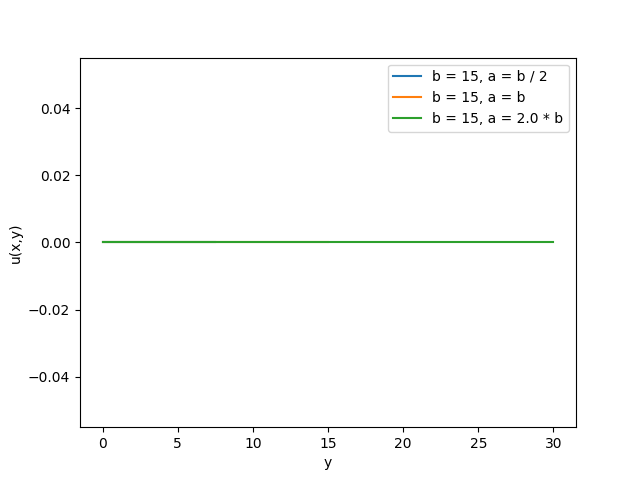
\includegraphics[width=1\textwidth, scale=0.8]{images/results/static_1/u(a,y).png}
        \caption{Переміщення $u(a, y)$}\label{static_1_u(a,y)}
    \end{center}
\end{figure}

Рис. \ref{static_1_u(a,y)} повністю підтверджує виконання граничної умови
\newline $u(x,y) |_{x=a}=0$.
Зауважимо, що на цьому графіку присутні всі три значення функції перемеіщення, які повністю накладаються одні на одну.

\begin{figure}[h!]
    \begin{center}
        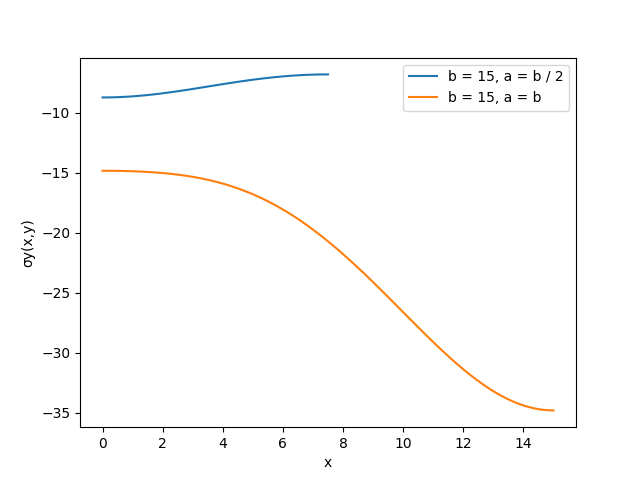
\includegraphics[width=0.49\textwidth, scale=1]{images/results/static_1/sigma_y(x,b:2)1.png}
        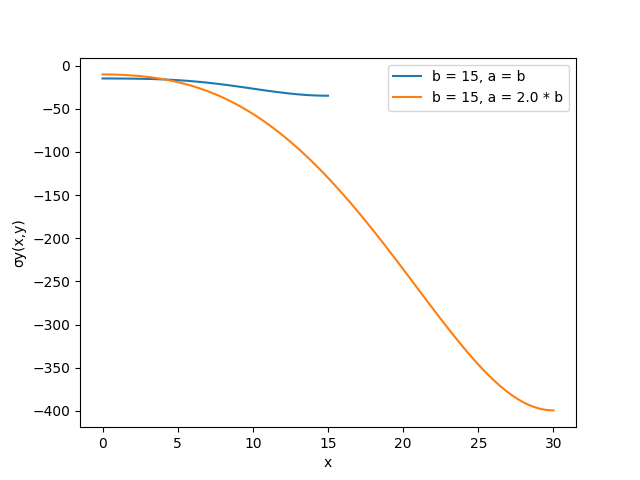
\includegraphics[width=0.49\textwidth, scale=1]{images/results/static_1/sigma_y(x,b:2)2.png}
        \caption{Напруження $\sigma_y(x, \frac{b}{2})$}\label{static_1_sigma_y(x,b:2)}
    \end{center}
\end{figure}

\begin{figure}[h!]
    \begin{center}
        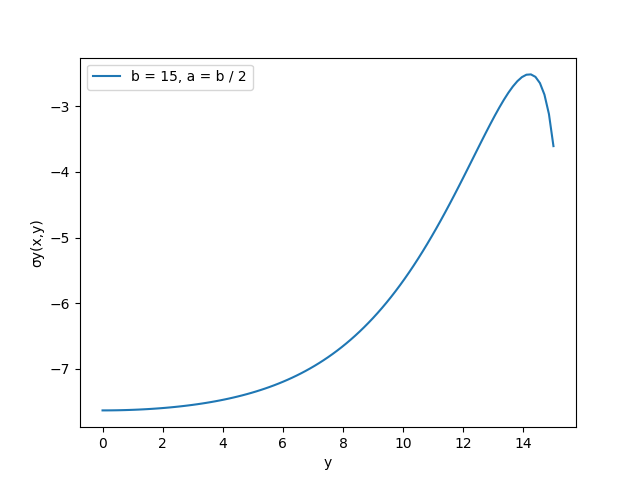
\includegraphics[width=0.49\textwidth, scale=1]{images/results/static_1/sigma_y(a,y)1.png}
        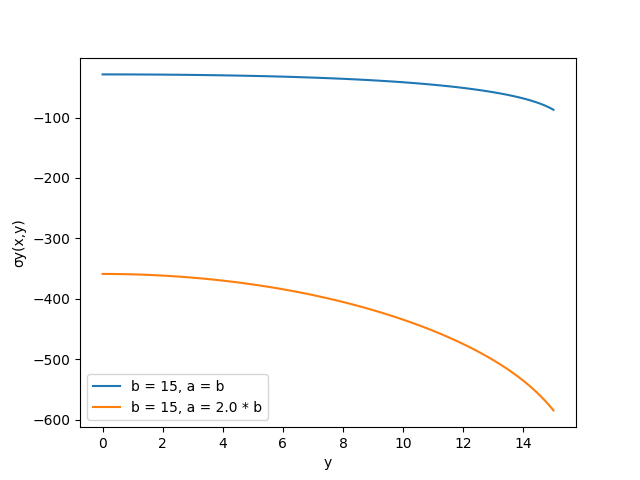
\includegraphics[width=0.49\textwidth, scale=1]{images/results/static_1/sigma_y(a,y)2.png}
        \caption{Напруження $\sigma_y(a, y)$}\label{static_1_sigma_y(a,y)}
    \end{center}
\end{figure}

\begin{figure}[h!]
    \begin{center}
        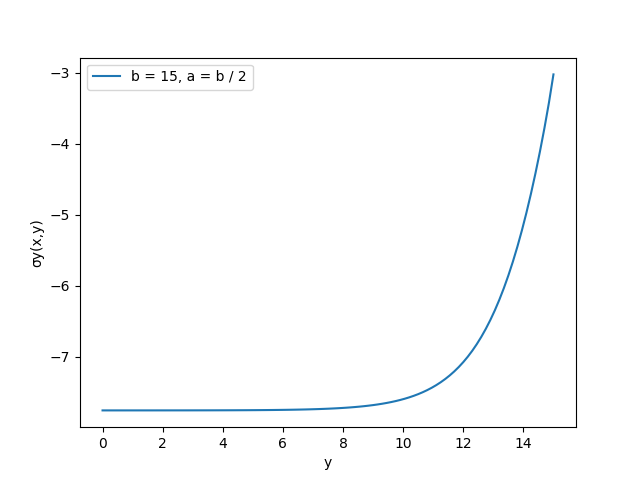
\includegraphics[width=0.49\textwidth, scale=1]{images/results/static_1/sigma_y(a:2,y)1.png}
        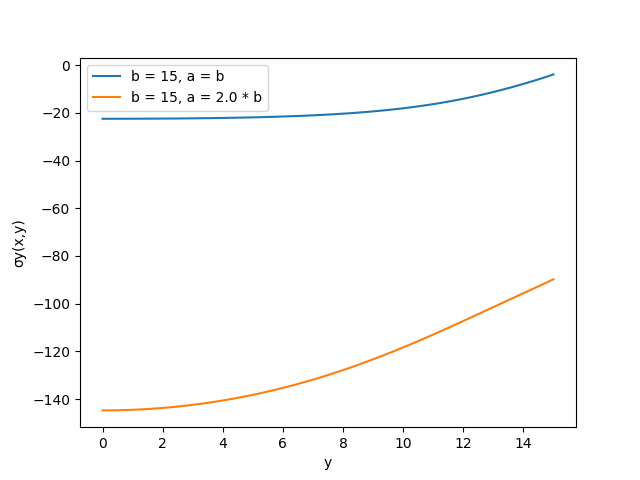
\includegraphics[width=0.49\textwidth, scale=1]{images/results/static_1/sigma_y(a:2,y)2.png}
        \caption{Напруження $\sigma_y(\frac{a}{2}, y)$}\label{static_1_sigma_y(a:2,y)}
    \end{center}
\end{figure}


\begin{figure}[h!]
    \begin{center}
        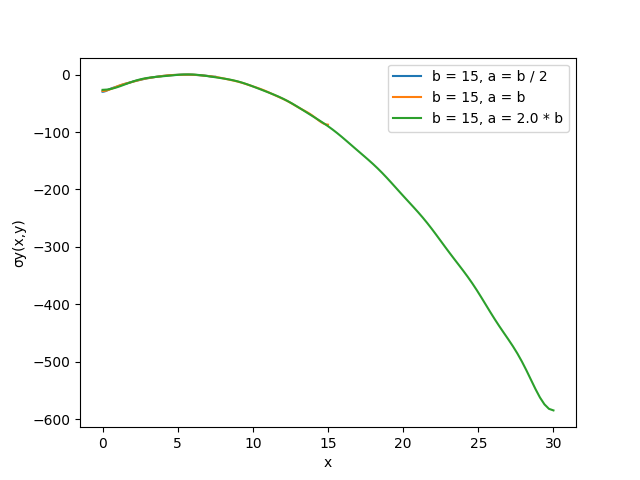
\includegraphics[width=1\textwidth, scale=1]{images/results/static_1/sigma_y(x,b).png}
        \caption{Напруження $\sigma_y(x, b)$}\label{static_1_sigma_y(x,b)}
    \end{center}
\end{figure}

З графіків Рис. \ref{static_1_sigma_y(x,b:2)} - \ref{static_1_sigma_y(x,b)} можна побачити,
що функції напруження в середині прямокутника (при $x=\frac{a}{2}$ або $y=\frac{b}{2}$)
міняють характер монотонності в залежності від розмірів геометричної області, а на гранях області (при $x=a$ або $y=b$)
характер залишається не змінним, лише міняються абсолютні значення функцій напружень.

Також на Рис. \ref{static_1_sigma_y(x,b)} видно, що функція напруження $\sigma_y(x,y)$ повністю задовольняє граничній умові при будь-яких розмірах області
та дорівнює значенню заданного навантаженню $p(x) = (x - 5.5)^2$ на грані $y=b$.
Зауважимо, що на цьому графіку також присутні всі три значення функції перемеіщення,
які повністю накладаються одні на одну,
як і в попередньому випадку.


\subsubsection{Випадок граничних умов другої основної задачі теорії пружності на бічних гранях}



\subsection{Динамічні задачі}
\newpage

\addcontentsline{toc}{section}{\protect\numberline{}Висновки}
\section*{\centering Висновки}
В дисертаційній роботі досліджено напружений стан та хвильові поля плоскої прямокутної області
під дією статичного та динамічного навантажень. За результатами дослідженя:
\begin{enumerate}
    \item Отримано методику аналітичного розв'язання задач теорії пружності для прямокутної області,
    що базується на застосувані методу інтегральних перетворень безпосередньо до рівнянь Ламе.
    Це дозволяє уникнути використання допоміжних функцій та сформулювати розв'язок у термінах механічних характеристик.

    \item Встановлено закономірності зміни напруженого стану прямокутної області в залежності від різних типів навантажень та різних типів граничних умов,
    які задано по її боковим торцях 

    \item Побудовано хвильові поля прямокутної пружної області та встановлено власні частоти тіла в залежності від типу динамічного навантаження на бокових торцях та геометричних розмірів області.
\end{enumerate}

Ці результати дозволили встановити такі особливості поведінки полів переміщень та напружень:
\begin{enumerate}
    \item 
\end{enumerate}
\newpage

\addcontentsline{toc}{section}{\protect\numberline{}СПИСОК ВИКОРИСТАНИХ ДЖЕРЕЛ}
\begin{thebibliography}{1}
    \bibitem{novacki_1}
    Nowacki W.: Teoria Sprezystosci. Panstwowe Wydawnictwo Naukowe, Warszawa (1970).
    \bibitem{vihak_1}
    V. M. Vihak, M. Y. Yuzvyak, A V. Yasinskij (1998) THE SOLUTION OF THE PLANE THERMOELASTICITY PROBLEM FOR A RECTANGULAR DOMAIN, Journal of Thermal Stresses, 21:5, 545-561, DOI: 10.1080/01495739808956162
    \bibitem{vihak_2}
    Vihak V. M., Tokovyy Yu. (2002) Construction elementary solutions of the elasticity plane problem for the rectangular domain. International applied mechanics. Volume 32, Issue 7, pp. 79-87.
    \bibitem{meleshko_1}
    Grinchenko, V.T. and Meleshko, V.V.: Harmonic Vibrations and Waves in Elastic Bodies [in Russian]. Naukova Dumka, Kiev (1981).
    \bibitem{kushnir_1}
    Kushnir, R.M., Yasinskyy, A.V., Tokovyy, Y.V. Reconstruction of the Thermal Load of a Functionally Graded Hollow Sphere by Surface Displacements. J Math Sci 270, 176–190 (2023). https://doi.org/10.1007/s10958-023-06339-8
    \bibitem{kreyn_1}
    Крейн М. Г. Интегральные уравнения на полупрямой с ядром, зависящим от разности аргументов // УМН. 1958. Т. 13, № 5. С. 3-120.
    \bibitem{zhuravleva_1}
    Zhuravlova Z. Yu. New approach of analytical inversion of Laplace transform for some cases. Researches in Mathematics and Mechanics 24, 122-135 (2019).
    \bibitem{popov_v_1}
    Popov, V.G., Lytvyn, O.V. Stress State of an Elastic Body with Rigid Inclusion in the Form of a Broken Line Under Harmonic Wave Loads. J Math Sci 263, 39–51 (2022). https://doi.org/10.1007/s10958-022-05905-w
    \bibitem{filshtin_1}
    L.A. Fil’shtinskii, Yu.V. Shramko, G.F. Burnatnaya: Model of the Elastic Plate Stiffened with the Regular System of Nanorods. J. Nano- Electron. Phys. 5 No 3, 03020 (2013) http://essuir.sumdu.edu.ua/handle/123456789/31952
    \bibitem{popov_1}
    Popov G., (1982) The elastic stress concentration around dies, cuts, thin, inclusions and reinforcements (in Russian), Nauka, Moscow.
    \bibitem{loboda_1}
    Loboda V. V., Sheveleva A. E. Steady thermal contact of a half strip and a strip // Inzhenerno-Fizicheskii Zhurnal. 1987. Vol. 53, No 2. P. 302-307.


    \bibitem{oden_1}
    Oden J. T., Kikuchi N. (1982) Finite element methods for constrained problems in elasticity. International journal for Numerical Methods in Engineering. Volume 18, Issue 5.
    \bibitem{babushka_1}
    Babuška, I. The finite element method with Lagrangian multipliers. Numer. Math. 20, 179–192 (1973). https://doi.org/10.1007/BF01436561
    \bibitem{maurizio_1}
    Maurizio A., A high-continuity finite element model for two-dimensional elastic problems. Computers and Structures, Volume 21, Issue 5 (1985), Pages 987-993, ISSN 0045-7949, https://doi.org/10.1016/0045-7949(85)90211-1.
    \bibitem{liew_1}
    Liew K. M., Yuming Cheng, Kitipornchai S. (2005) Boundary element-free method (BEFM) and application to two dimensional elasticity problems. International journal for Numerical Methods in Engineering. Vulume 65, Issue 8.
    \bibitem{dong_1}
    Dongyang Shi, Minghao Li, (2014) Superconvergence analysis of the stable conforming rectangular mixed nite elements for the linear elasticity problem Journal of Computati- onal Mathematics. Volume 32, Number 2, pp. 205-214.
    \bibitem{golovchan_1}
    Golovchan, V.T. On the solution of plane boundary-value problems of elasticity in a rectangle. Int Appl Mech 42, 84–89 (2006). https://doi.org/10.1007/s10778-006-0061-8
    
    \bibitem{shyam_1}
    Shyam N. Prasad, Sailendra N. Chatterjee (1973) Some mixed boundary value problems of elasticity in a rectangular domain. International journal of Solids and Structures. Volume 9, Issue 10, pp. 1193-1210.
    \bibitem{kovalenko_1}
    Kovalenko, M.D., Menshova, I.V., Kerzhaev, A.P. et al. A boundary value problem in the theory of elasticity for a rectangle: exact solutions. Z. Angew. Math. Phys. 71, 199 (2020). https://doi.org/10.1007/s00033-020-01425-2
    \bibitem{bantsuri_1}
    Bantsuri, R., Mzhavanadze, Sh. (2007). The mixed problem of the theory of elasticity for a rectangle weakened by unknown equiv-string holes. Proceedings of A. Razmadze Mathematical Institute. 145. 
    \bibitem{kashtalyan_1}
    M Kashtalyan, Three-dimensional elasticity solution for bending of functionally graded rectangular plates, European Journal of Mechanics - A/Solids, Volume 23, Issue 5, 2004, Pages 853-864, ISSN 0997-7538, https://doi.org/10.1016/j.euromechsol.2004.04.002.
    \bibitem{zhuk_1}
    Zhuk, Y.O., Ostos, O.K., Karnaukhova, T.V. Forced Vibrations and Nonstationary Heating of a Rectangular Viscoelastic Plate with Prestresses. Int Appl Mech 58, 423–435 (2022). https://doi.org/10.1007/s10778-022-01167-w
    \bibitem{maksymuk_1}
    Maksymuk, O.V., Sachuk, Y.V., Yatsyuk, S.M. Plane Contact Problems for an Elastic Foundation with Two Bedding Coefficients. J Math Sci 273, 153–162 (2023). https://doi.org/10.1007/s10958-023-06491-1

    \bibitem{popov_4}
    Попов Г. Я. Концентрация упругих напряжений возле штампов разрезов тонких включений и подкреплений. М.: Наука. Главная редакция физико-математической литературы, 1982. 344 с.
    \bibitem{popov_5}
    Попов Г. Я., Абдыманов С. А., Ефимов В. В. Функции и матрицы Грина одномерных краевых задач. Алматы: Изд. Рацах, 1999. 133 с.

    \bibitem{popov_2}
    Попов Г.Я. Точные решения некоторых краевых задач механики деформируемого твѐрдого тела. Одесса: Астропринт, 2013. 424 с.
    \bibitem{popov_3}
    Popov G. On the method of orthogonal polynomials in contact problems of the theory of elasticity. Journal of Applied Mathematics and Mechanics (1969). Volume 33, Issue 3, pp. 503-517
    \bibitem{gantmaher}
    Gantmakher F. R. (1998) The theory of matrices. AMS Chelsea Publishing, Providence, Rohde Island.
    \bibitem{ortogonal}
    Попов Г. Я., Реут В. В., Моісеєв М. Г., Вайсфельд Н. Д. Рівняння математичної фізики. Метод ортогональних многочленів. Одесса: Астропринт, 2010. 120 с.
    \bibitem{prudnikov}
    Прудников А.П.,Брычков Ю.А., Маричев О.И. Интегралы и ряды специальные функции. В 3 т. Т 1. Элементарные функции. 2-е издание, исправленное. М.: ФИЗМАТЛИТ, 2002. 632 с.
    \bibitem{pozhylenkov_1}
    D. Nerukh, O. Pozhylenkov, N. Vaysfeld (2019) Mixed plain boundary value problem of elasticity for a rectangular domain. 25-th International Conference Engineering Mechanics. 2019, May 13-16, Svratka, Czech Republic. p. 255
    \bibitem{pozhylenkov_2}
    O. V. Pozhylenkov (2019) The stress state of a rectangular elastic domain. Researches in Mathematics and Mechanics, Volume 24, Issue 2(34), pp. 88-96
    \bibitem{pozhylenkov_3}
    Пожиленков О. В. Вайсфельд Н. Д. (2019) Мішана крайова задача теорії пружності для прямокутної області. Математичні проблеми механіки неоднорідних структур, випуск 5, Львів, ст. 30-32
    \bibitem{conf_1}
    D. Nerukh, O. Pozhylenkov, N. Vaysfeld 25-th international conference «Engineering Mechanics 2019» // Czech Republic, Svratka, 2019
    \bibitem{conf_2}
    Пожиленков О. В., Вайсфельд Н. Д. Х Мiжнародна наукова конференцiя «Математичнi проблеми механiки неоднорiдних структур» // Львiв, 2019
    \bibitem{pozhylenkov_4}
    O. Pozhyenkov, N. Vaysfeld (2020) Stress state of a rectangular domain with the mixed boundary conditions. Procedia Structural Integrity, Volume 28, pp. 458-463
    \bibitem{conf_3}
    O. Pozhyenkov, N. Vaysfeld «1st Virtual European Conference on Fracture» // Italy, 2020
    \bibitem{pozhylenkov_5}
    O. Pozhyenkov, N. Vaysfeld (2021) Stress state of an elastic rectangular domain under steady load. Procedia Structural Integrity, Volume 33, pp. 385-390
    \bibitem{conf_4}
    O. Pozhyenkov, N. Vaysfeld «26th International Conference on Fracture and Structural Integrity» // Italy, Turin, 2021
    \bibitem{pozhylenkov_6}
    O. Pozhylenkov, N. Vaysfeld (2022) Dynamic mixed problem of elasticity for a rectangular domain. Recent trends in Wave Mechanics and Vibrations, pp. 211-218
    \bibitem{conf_5}
    O. Pozhyenkov, N. Vaysfeld «10th International Conference on Wave Mechanics and Vibrations» // Portugal, Lisbon, 2022
\end{thebibliography}
\newpage

\addcontentsline{toc}{section}{\protect\numberline{}Додаток B ЗНАХОДЖЕННЯ КОРЕНІВ РІВНЯННЯ $det[M(s)]=0$}
\section*{\centering Додаток B}\label{ap_B}
\section*{\centering ЗНАХОДЖЕННЯ КОРЕНІВ РІВНЯННЯ $det[M(s)]=0$}
Знайдемо корені $det[M(s)]=0$
\begin{align*}
    &det[M(s)] = (s^2 (1 + \mu_0) -\alpha_n^2 + \frac{\omega^2}{c_2^2})(s^2 - \alpha_n^2 - \alpha_n^2\mu_0 + \frac{\omega^2}{c_1^2}) + (\alpha_n \mu_0 s)^2 = \\
    &= s^4 + s^4 \mu_0 - s^2 \alpha_n^2 + s^2 \frac{\omega^2}{c_2^2} - s^2 \alpha_n^2 - s^2 \alpha_n^2 \mu_0 + \alpha_n^4 - \alpha_n^2 \frac{\omega^2}{c_2^2} - s^2 \alpha_n^2 \mu_0 - \\
    &- s^2 \alpha_n^2 \mu_0 + \alpha_n^4 \mu_0 - \alpha_n^2 \frac{\omega^2}{c_2^2} + s^2 \frac{\omega^2}{c_1^2} + s^2 \mu_0 \frac{\omega^2}{c_1^2} - \alpha_n^2 \frac{\omega^2}{c_1^2} + \frac{\omega^4}{c_1^2 c_2^2} + s^2 \alpha_n^2 \mu_0^2 = \\
    &=(1 + \mu_0) s^4 + (-2 \alpha_n^2 - 2 \alpha_n^2 \mu_0 + \frac{\omega^2}{c_2^2} + \frac{\omega^2}{c_1^2} + \mu_0 \frac{\omega^2}{c_1^2}) s^2 + (\alpha_n^4 - \alpha_n^2 \frac{\omega^2}{c_2^2} + \\ 
    &+ \alpha_n^4 \mu_0 - \alpha_n^2 \mu_0 \frac{\omega^2}{c_2^2} - \alpha_n^2 \frac{\omega^2}{c_1^2} + \frac{\omega^4}{c_1^2 c_2^2})
\end{align*}
Введемо наступні позначення:
\begin{align*}
    &a_1 = -2 \alpha_n^2 - 2 \alpha_n^2 \mu_0 + \frac{\omega^2}{c_2^2} + \frac{\omega^2}{c_1^2} + \mu_0 \frac{\omega^2}{c_1^2} \\
    &a_2 = \alpha_n^4 - \alpha_n^2 \frac{\omega^2}{c_2^2} + \alpha_n^4 \mu_0 - \alpha_n^2 \mu_0 \frac{\omega^2}{c_2^2} - \alpha_n^2 \frac{\omega^2}{c_1^2} + \frac{\omega^4}{c_1^2 c_2^2}
\end{align*}
Враховучи введені позначення отримаємо наступне рівняння:
\begin{equation*}
    (1 + \mu_0) s^4 + a_1 s^2 + a_2 = 0
\end{equation*}
Таким чином отримаємо наступні корені рівняння:
\begin{align*}
    &s_1 = \sqrt{\frac{ -a_1 + \sqrt{a_1^2 - 4(1 + \mu_0)a_2}}{2 (1 + \mu_0)}} \\
    &s_2 = -\sqrt{\frac{ -a_1 + \sqrt{a_1^2 - 4(1 + \mu_0)a_2}}{2 (1 + \mu_0)}} \\
    &s_3 = \sqrt{\frac{ -a_1 - \sqrt{a_1^2 - 4(1 + \mu_0)a_2}}{2 (1 + \mu_0)}} \\
    &s_4 = -\sqrt{\frac{ -a_1 - \sqrt{a_1^2 - 4(1 + \mu_0)a_2}}{2 (1 + \mu_0)}}
\end{align*}
У випадку статичної задачі ($\omega = 0$) отримаємо наступні рівняння:
\begin{equation*}
    (1 + \mu_0) (s^4 - 2 \alpha_n^2 s^2 + \alpha_n^4) = 0
\end{equation*}
Таким чином отримаємо наступні корені
\begin{align*}
    &s_{1,2} = \alpha_n \\
    &s_{3, 4} = -\alpha_n
\end{align*}

\newpage

\addcontentsline{toc}{section}{\protect\numberline{}Додаток C ЗНАХОДЖЕННЯ ФУНДАМЕНТАЛЬНИХ БАЗИСНИХ МАТРИЦЬ $\Psi_i(y)$, $i=\overline{0,1}$}
\section*{\centering Додаток C}\label{ap_C}
\section*{\centering ЗНАХОДЖЕННЯ ФУНДАМЕНТАЛЬНИХ БАЗИСНИХ МАТРИЦЬ $\Psi_i(y)$, $i=\overline{0,1}$}
Для знаходження фундаентальних базісних матриць $\Psi_i(y)$
випишемо умови за яких будемо шукати коєфіцієти $C_k^i$, $i=\overline{0,1}$, $k=\overline{1,2}$
\begin{align*}\tag{Aп.С. 1}\label{ap_c_bound}
    &U_0\left[ \Psi_0(y) \right] = I, \quad U_1\left[ \Psi_0(y) \right] = 0 \\
    &U_0\left[ \Psi_1(y) \right] = 0, \quad U_1\left[ \Psi_1(y) \right] = I, \quad I = \begin{pmatrix}
        1 && 0 \\
        0 && 1
    \end{pmatrix} \\
    &U_0\left[ \Psi_i(y) \right] =  \begin{pmatrix}
        1 & 0 \\
        0 & 2G + \lambda
    \end{pmatrix} * \Psi_i^{'}(b) + \begin{pmatrix}
        0 & -\alpha_n \\
        \alpha_n \lambda & 0
    \end{pmatrix} * \Psi_i(b) \\
    &U_1\left[ \Psi_i(y) \right] =  \begin{pmatrix}
        1 & 0 \\
        0 & 0
    \end{pmatrix} * \Psi_i^{'}(0) + \begin{pmatrix}
        0 & -\alpha_n \\
        0 & 1
    \end{pmatrix} * \Psi_i(0) \\
\end{align*}

Введемо наступні позначення:
\begin{equation*}\tag{Aп.С. 2}\label{ap_c_coef}
    C_1^i = \begin{pmatrix}
        d_1^i && d_2^i \\
        d_3^i && d_4^i
    \end{pmatrix}, \quad
    C_2^i = \begin{pmatrix}
        f_1^i && f_2^i \\
        f_3^i && f_4^i
    \end{pmatrix},
\end{equation*}

\subsection*{Випадок динамічної задачі}
Випадку статичної задачі випишемо значення елементів матриць $\Psi_i(y)$, $\Psi_i^{'}(y)$, враховуючи позначення \eqref{ap_c_coef}.

Елементи матриці $\Psi_i(y)$:
\begin{align*}
    &\Psi_i(y)_{1,1}= \frac{1}{2 s_1 (s_1^2 - s_2^2)} [(s_1^2 + s_1^2 \mu_0 - \alpha_n^2 + \frac{\omega^2}{c_2^2}) (e^{s_1 y} - e^{-s_1 y}) d_1^i + \\
    &+ (s_1 \alpha_n \mu_0) (e^{s_1 y} + e^{-s_1 y}) d_3^i ]
    + [(s_2^2 + s_2^2 \mu_0 - \alpha_n^2 + \frac{\omega^2}{c_2^2}) (e^{s_2 y} - e^{-s_2 y}) f_1^i + \\
    &+ (s_2 \alpha_n \mu_0) (e^{s_2 y} + e^{-s_2 y}) f_3^i ] \frac{1}{2 s_2 (s_2^2 - s_1^2)}
\end{align*}
\begin{align*}
    &\Psi_i(y)_{1,2}= \frac{1}{2 s_1 (s_1^2 - s_2^2)} [(s_1^2 + s_1^2 \mu_0 - \alpha_n^2 + \frac{\omega^2}{c_2^2}) (e^{s_1 y} - e^{-s_1 y}) d_2^i + \\
    &+ (s_1 \alpha_n \mu_0) (e^{s_1 y} + e^{-s_1 y}) d_4^i ]
    + [(s_2^2 + s_2^2 \mu_0 - \alpha_n^2 + \frac{\omega^2}{c_2^2}) (e^{s_2 y} - e^{-s_2 y}) f_2^i + \\
    &+ (s_2 \alpha_n \mu_0) (e^{s_2 y} + e^{-s_2 y}) f_4^i ] \frac{1}{2 s_2 (s_2^2 - s_1^2)}
\end{align*}
\begin{align*}
    &\Psi_i(y)_{2,1}= \frac{1}{2 s_1 (s_1^2 - s_2^2)} [(-s_1 \alpha_n \mu_0) (e^{s_1 y} + e^{-s_1 y}) d_1^i + \\
    &+ (s_1^2 - \alpha_n^2 - \alpha_n^2\mu_0 + \frac{\omega^2}{c_1^2}) (e^{s_1 y} - e^{-s_1 y}) d_3^i ]
    + [(-s_2 \alpha_n \mu_0) (e^{s_2 y} + e^{-s_2 y}) f_1^i + \\
    &+ (s_2^2 - \alpha_n^2 - \alpha_n^2\mu_0 + \frac{\omega^2}{c_1^2}) (e^{s_2 y} - e^{-s_2 y}) f_3^i ] \frac{1}{2 s_2 (s_2^2 - s_1^2)}
\end{align*}
\begin{align*}
    &\Psi_i(y)_{2,2}= \frac{1}{2 s_1 (s_1^2 - s_2^2)} [(-s_1 \alpha_n \mu_0) (e^{s_1 y} + e^{-s_1 y}) d_2^i + \\
    &+ (s_1^2 - \alpha_n^2 - \alpha_n^2\mu_0 + \frac{\omega^2}{c_1^2}) (e^{s_1 y} - e^{-s_1 y}) d_4^i ]
    + [(-s_2 \alpha_n \mu_0) (e^{s_2 y} + e^{-s_2 y}) f_2^i + \\
    &+ (s_2^2 - \alpha_n^2 - \alpha_n^2\mu_0 + \frac{\omega^2}{c_1^2}) (e^{s_2 y} - e^{-s_2 y}) f_4^i ] \frac{1}{2 s_2 (s_2^2 - s_1^2)}
\end{align*}
Елементи матриці $\Psi_i^{'}(y)$:
\begin{align*}
    &\Psi_i^{'}(y)_{1,1}= \frac{1}{2 (s_1^2 - s_2^2)} [(s_1^2 + s_1^2 \mu_0 - \alpha_n^2 + \frac{\omega^2}{c_2^2}) (e^{s_1 y} + e^{-s_1 y}) d_1^i + \\
    &+ (s_1 \alpha_n \mu_0) (e^{s_1 y} - e^{-s_1 y}) d_3^i ]
    + [(s_2^2 + s_2^2 \mu_0 - \alpha_n^2 + \frac{\omega^2}{c_2^2}) (e^{s_2 y} + e^{-s_2 y}) f_1^i + \\
    &+ (s_2 \alpha_n \mu_0) (e^{s_2 y} - e^{-s_2 y}) f_3^i ] \frac{s_2}{2 s_2 (s_2^2 - s_1^2)}
\end{align*}
\begin{align*}
    &\Psi_i^{'}(y)_{1,2}= \frac{1}{2 (s_1^2 - s_2^2)} [(s_1^2 + s_1^2 \mu_0 - \alpha_n^2 + \frac{\omega^2}{c_2^2}) (e^{s_1 y} + e^{-s_1 y}) d_2^i + \\
    &+ (s_1 \alpha_n \mu_0) (e^{s_1 y} - e^{-s_1 y}) d_4^i ]
    + [(s_2^2 + s_2^2 \mu_0 - \alpha_n^2 + \frac{\omega^2}{c_2^2}) (e^{s_2 y} + e^{-s_2 y}) f_2^i + \\
    &+ (s_2 \alpha_n \mu_0) (e^{s_2 y} - e^{-s_2 y}) f_4^i ] \frac{s_2}{2 s_2 (s_2^2 - s_1^2)}
\end{align*}
\begin{align*}
    &\Psi_i^{'}(y)_{2,1}= \frac{1}{2 (s_1^2 - s_2^2)} [(-s_1 \alpha_n \mu_0) (e^{s_1 y} - e^{-s_1 y}) d_1^i + \\
    &+ (s_1^2 - \alpha_n^2 - \alpha_n^2\mu_0 + \frac{\omega^2}{c_1^2}) (e^{s_1 y} + e^{-s_1 y}) d_3^i ]
    + [(-s_2 \alpha_n \mu_0) (e^{s_2 y} - e^{-s_2 y}) f_1^i + \\
    &+ (s_2^2 - \alpha_n^2 - \alpha_n^2\mu_0 + \frac{\omega^2}{c_1^2}) (e^{s_2 y} + e^{-s_2 y}) f_3^i ] \frac{s_2}{2 s_2 (s_2^2 - s_1^2)}
\end{align*}
\begin{align*}
    &\Psi_i^{'}(y)_{2,2}= \frac{1}{2 (s_1^2 - s_2^2)} [(-s_1 \alpha_n \mu_0) (e^{s_1 y} - e^{-s_1 y}) d_2^i + \\
    &+ (s_1^2 - \alpha_n^2 - \alpha_n^2\mu_0 + \frac{\omega^2}{c_1^2}) (e^{s_1 y} + e^{-s_1 y}) d_4^i ]
    + [(-s_2 \alpha_n \mu_0) (e^{s_2 y} - e^{-s_2 y}) f_2^i + \\
    &+ (s_2^2 - \alpha_n^2 - \alpha_n^2\mu_0 + \frac{\omega^2}{c_1^2}) (e^{s_2 y} + e^{-s_2 y}) f_4^i ] \frac{s_2}{2 s_2 (s_2^2 - s_1^2)}
\end{align*}
Введемо наступні позначення:
\begin{align*}\tag{Aп.C. 3}\label{ap_c_def_dynamic}
    &a_1(y) = \frac{(s_1^2 + s_1^2 \mu_0 - \alpha_n^2 + \frac{\omega^2}{c_2^2}) (e^{s_1 y} - e^{-s_1 y})}{2 s_1 (s_1^2 - s_2^2)}, \\ 
    &a_2(y) = \frac{(s_1 \alpha_n \mu_0) (e^{s_1 y} + e^{-s_1 y})}{2 s_1 (s_1^2 - s_2^2)} \\
    &a_3(y) = \frac{(s_2^2 + s_2^2 \mu_0 - \alpha_n^2 + \frac{\omega^2}{c_2^2}) (e^{s_2 y} - e^{-s_2 y})}{2 s_2 (s_2^2 - s_1^2)}, \\
    &a_4(y) = \frac{(s_2 \alpha_n \mu_0) (e^{s_2 y} + e^{-s_2 y})}{2 s_2 (s_2^2 - s_1^2)} \\
    &a_5(y) = \frac{(-s_1 \alpha_n \mu_0) (e^{s_1 y} + e^{-s_1 y})}{2 s_1 (s_1^2 - s_2^2)}, \\
    &a_6(y) = \frac{(s_1^2 - \alpha_n^2 - \alpha_n^2\mu_0 + \frac{\omega^2}{c_1^2}) (e^{s_1 y} - e^{-s_1 y})}{2 s_1 (s_1^2 - s_2^2)} \\
    &a_7(y) = \frac{(-s_2 \alpha_n \mu_0) (e^{s_2 y} - e^{-s_2 y})}{2 s_2 (s_2^2 + s_1^2)}, \\
    &a_8(y) = \frac{(s_2^2 - \alpha_n^2 - \alpha_n^2\mu_0 + \frac{\omega^2}{c_1^2}) (e^{s_2 y} - e^{-s_2 y})}{2 s_2 (s_2^2 - s_1^2)} \\
    &a_9(y) = \frac{(s_1^2 + s_1^2 \mu_0 - \alpha_n^2 + \frac{\omega^2}{c_2^2}) (e^{s_1 y} + e^{-s_1 y})}{2 (s_1^2 - s_2^2)}, \\
    &a_{10}(y) = \frac{(s_1 \alpha_n \mu_0) (e^{s_1 y} - e^{-s_1 y})}{2 (s_1^2 - s_2^2)} \\
    &a_{11}(y) = \frac{(s_2^2 + s_2^2 \mu_0 - \alpha_n^2 + \frac{\omega^2}{c_2^2}) (e^{s_2 y} + e^{-s_2 y})}{2 (s_2^2 - s_1^2)}, \\ 
    &a_{12}(y) = \frac{(s_2 \alpha_n \mu_0) (e^{s_2 y} - e^{-s_2 y})}{2 (s_2^2 - s_1^2)} \\
    &a_{13}(y) = \frac{(-s_1 \alpha_n \mu_0) (e^{s_1 y} - e^{-s_1 y})}{2 (s_1^2 - s_2^2)}, \\ 
    &a_{14}(y) = \frac{(s_1^2 - \alpha_n^2 - \alpha_n^2\mu_0 + \frac{\omega^2}{c_1^2}) (e^{s_1 y} + e^{-s_1 y})}{2 (s_1^2 - s_2^2)} \\
    &a_{15}(y) = \frac{(-s_2 \alpha_n \mu_0) (e^{s_2 y} - e^{-s_2 y})}{2 (s_2^2 - s_1^2)}, \\ 
    &a_{16}(y) = \frac{(s_2^2 - \alpha_n^2 - \alpha_n^2\mu_0 + \frac{\omega^2}{c_1^2}) (e^{s_2 y} + e^{-s_2 y})}{2 (s_2^2 - s_1^2)}
\end{align*}

\subsection*{Випадок статичної задачі}
Випадку статичної задачі випишемо значення елементів матриць $\Psi_i(y)$, $\Psi_i^{'}(y)$, враховуючи позначення \eqref{ap_c_coef}.

Елементи матриці $\Psi_i(y)$:
\begin{align*}
    &\Psi_i(y)_{1,1}=  \frac{e^{\alpha_n y}}{(1 + \mu_0) 4 \alpha_n} \left[ (y \alpha_n \mu_0 + 2 + \mu_0)d_1^i + (y \alpha_n \mu_0)d_3^i \right] + \\ 
    &+ \frac{e^{-\alpha_n y}}{(1 + \mu_0) 4 \alpha_n} \left[ (y \alpha_n \mu_0 - 2 - \mu_0) f_1^i + (-y \alpha_n \mu_0) f_3^i \right]
\end{align*}
\begin{align*}
    &\Psi_i(y)_{1,2}=  \frac{e^{\alpha_n y}}{(1 + \mu_0) 4 \alpha_n} \left[ (y \alpha_n \mu_0 + 2 + \mu_0)d_2^i + (y \alpha_n \mu_0)d_4^i \right] + \\ 
    &+ \frac{e^{-\alpha_n y}}{(1 + \mu_0) 4 \alpha_n} \left[ (y \alpha_n \mu_0 - 2 - \mu_0) f_2^i + (-y \alpha_n \mu_0) f_4^i \right]
\end{align*}
\begin{align*}
    &\Psi_i(y)_{2,1}=  \frac{e^{\alpha_n y}}{(1 + \mu_0) 4 \alpha_n} \left[ (-y \alpha_n \mu_0) d_1^i + (-y \alpha_n \mu_0 + 2 + \mu_0) d_3^i \right] + \\ 
    &+ \frac{e^{-\alpha_n y}}{(1 + \mu_0) 4 \alpha_n} \left[ (y \alpha_n \mu_0) f_1^i + (-y \alpha_n \mu_0 - 2 - \mu_0) f_3^i \right]
\end{align*}
\begin{align*}
    &\Psi_i(y)_{2,2}=  \frac{e^{\alpha_n y}}{(1 + \mu_0) 4 \alpha_n} \left[ (-y \alpha_n \mu_0) d_2^i + (-y \alpha_n \mu_0 + 2 + \mu_0) d_4^i \right] + \\ 
    &+ \frac{e^{-\alpha_n y}}{(1 + \mu_0) 4 \alpha_n} \left[ (y \alpha_n \mu_0) f_2^i + (-y \alpha_n \mu_0 - 2 - \mu_0) f_4^i \right]
\end{align*}
Елементи матриці $\Psi_i^{'}(y)$:
\begin{align*}
    &\Psi_i^{'}(y)_{1,1}=  \frac{e^{\alpha_n y}}{(1 + \mu_0) 4} \left[ (y \alpha_n \mu_0 + 2 + 2 \mu_0)d_1^i + (y \alpha_n \mu_0 + \mu_0)d_3^i \right] + \\ 
    &+ \frac{e^{-\alpha_n y}}{(1 + \mu_0) 4} \left[ (-y \alpha_n \mu_0 + 2 + 2 \mu_0) f_1^i + (y \alpha_n \mu_0 - \mu_0) f_3^i \right]
\end{align*}
\begin{align*}
    &\Psi_i^{'}(y)_{1,2}=  \frac{e^{\alpha_n y}}{(1 + \mu_0) 4} \left[ (y \alpha_n \mu_0 + 2 + 2 \mu_0)d_2^i + (y \alpha_n \mu_0 + \mu_0)d_4^i \right] + \\ 
    &+ \frac{e^{-\alpha_n y}}{(1 + \mu_0) 4} \left[ (-y \alpha_n \mu_0 + 2 + 2 \mu_0) f_2^i + (y \alpha_n \mu_0 - \mu_0) f_4^i \right]
\end{align*}
\begin{align*}
    &\Psi_i^{'}(y)_{2,1}=  \frac{e^{\alpha_n y}}{(1 + \mu_0) 4} \left[ (-y \alpha_n \mu_0 - \mu_0) d_1^i + (-y \alpha_n \mu_0 + 2) d_3^i \right] + \\ 
    &+ \frac{e^{-\alpha_n y}}{(1 + \mu_0) 4} \left[ (-y \alpha_n \mu_0 + \mu_0) f_1^i + (y \alpha_n \mu_0 + 2) f_3^i \right]
\end{align*}
\begin{align*}
    &\Psi_i^{'}(y)_{2,2}=  \frac{e^{\alpha_n y}}{(1 + \mu_0) 4} \left[ (-y \alpha_n \mu_0 - \mu_0) d_2^i + (-y \alpha_n \mu_0 + 2) d_4^i \right] + \\ 
    &+ \frac{e^{-\alpha_n y}}{(1 + \mu_0) 4} \left[ (-y \alpha_n \mu_0 + \mu_0) f_2^i + (y \alpha_n \mu_0 + 2) f_4^i \right]
\end{align*}
Введемо наступні позначення:
\begin{align*}\tag{Ап.C. 4}\label{ap_c_def_static}
    &a_1(y) = \frac{e^{\alpha_n y} (y \alpha_n \mu_0 + 2 + \mu_0)}{(1 + \mu_0) 4 \alpha_n}, \quad a_2(y) = \frac{e^{\alpha_n y} (y \alpha_n \mu_0)}{(1 + \mu_0) 4 \alpha_n} \\
    &a_3(y) = \frac{e^{-\alpha_n y} (y \alpha_n \mu_0 - 2 - \mu_0)}{(1 + \mu_0) 4 \alpha_n}, \quad a_4(y) =  \frac{e^{-\alpha_n y} (-y \alpha_n \mu_0)}{(1 + \mu_0) 4 \alpha_n} \\
    &a_5(y) = \frac{e^{\alpha_n y} (-y \alpha_n \mu_0)}{(1 + \mu_0) 4 \alpha_n}, \quad a_6(y) = \frac{e^{\alpha_n y} (-y \alpha_n \mu_0 + 2 + \mu_0)}{(1 + \mu_0) 4 \alpha_n} \\
    &a_7(y) = \frac{e^{-\alpha_n y} (y \alpha_n \mu_0)}{(1 + \mu_0) 4 \alpha_n}, \quad a_8(y) = \frac{e^{-\alpha_n y}  (-y \alpha_n \mu_0 - 2 - \mu_0)}{(1 + \mu_0) 4 \alpha_n} \\
    &a_9(y) = \frac{e^{\alpha_n y} (y \alpha_n \mu_0 + 2 + 2 \mu_0)}{(1 + \mu_0) 4}, \quad a_{10}(y) = \frac{e^{\alpha_n y} (y \alpha_n \mu_0 + \mu_0)}{(1 + \mu_0) 4} \\
    &a_{11}(y) = \frac{e^{-\alpha_n y} (-y \alpha_n \mu_0 + 2 + 2 \mu_0)}{(1 + \mu_0) 4}, \quad a_{12}(y) = \frac{e^{-\alpha_n y} (y \alpha_n \mu_0 - \mu_0)}{(1 + \mu_0) 4} \\
    &a_{13}(y) = \frac{e^{\alpha_n y} (-y \alpha_n \mu_0 - \mu_0)}{(1 + \mu_0) 4}, \quad a_{14}(y) = \frac{e^{\alpha_n y} (-y \alpha_n \mu_0 + 2)}{(1 + \mu_0) 4} \\
    &a_{15}(y) = \frac{e^{-\alpha_n y} (-y \alpha_n \mu_0 + \mu_0)}{(1 + \mu_0) 4}, \quad a_{16}(y) = \frac{e^{-\alpha_n y} (y \alpha_n \mu_0 + 2)}{(1 + \mu_0) 4}
\end{align*}

\subsection*{Загальна схема побудови систем алгребричних рівнянь}
Враховуючи введені позначення \eqref{ap_c_def_dynamic}, \eqref{ap_c_def_static} складемо систему алгебричних рівнянь використовуючи граничні умови \eqref{ap_c_bound}.
Запишемо елементи вихідної матриці $U_0\left[ \Psi_i(y) \right]$:
\begin{align*}
    &U_0\left[ \Psi_i(y) \right]_{1,1} = (a_9(b) - \alpha_n a_5(b)) d_1^i + (a_{10}(b) - \alpha_n a_6(b)) d_3^i + \\
    &+ (a_{11}(b) - \alpha_n a_7(b)) f_1^i + (a_{12}(b) - \alpha_n a_8(b)) f_3^i 
\end{align*}
\begin{align*}
    &U_0\left[ \Psi_i(y) \right]_{1,2} = (a_9(b) - \alpha_n a_5(b)) d_2^i + (a_{10}(b) - \alpha_n a_6(b)) d_4^i + \\
    &+ (a_{11}(b) - \alpha_n a_7(b)) f_2^i + (a_{12}(b) - \alpha_n a_8(b)) f_4^i 
\end{align*}
\begin{align*}
    &U_0\left[ \Psi_i(y) \right]_{2,1} = ((2G + \lambda) a_{13}(b) + \alpha_n \lambda a_1(b)) d_1^i + \\ 
    &+ ((2G + \lambda) a_{14}(b) + \alpha_n \lambda a_2(b)) d_3^i + ((2G + \lambda)a_{15} + \alpha_n \lambda a_3(b)) f_1^i + \\ 
    &+ ((2G + \lambda)a_{16}(b) + \alpha_n \lambda a_4(b)) f_3^i 
\end{align*}
\begin{align*}
    &U_0\left[ \Psi_i(y) \right]_{2,2} = ((2G + \lambda) a_{13}(b) + \alpha_n \lambda a_1(b)) d_2^i + \\
    &+ ((2G + \lambda) a_{14}(b) + \alpha_n \lambda a_2(b)) d_4^i + ((2G + \lambda)a_{15} + \alpha_n \lambda a_3(b)) f_2^i + \\
    &+ ((2G + \lambda)a_{16}(b) + \alpha_n \lambda a_4(b)) f_4^i 
\end{align*}
Записано елементи вихідної матриці $U_1\left[ \Psi_i(y) \right]$:
\begin{align*}
    &U_1\left[ \Psi_i(y) \right]_{1,1} = (a_9(0) - \alpha_n a_5(0)) d_1^i + (a_{10}(0) - \alpha_n a_6(0)) d_3^i + \\
    &+ (a_{11}(0) - \alpha_n a_7(0)) f_1^i + (a_{12}(0) - \alpha_n a_8(0)) f_3^i 
\end{align*}
\begin{align*}
    &U_1\left[ \Psi_i(y) \right]_{1,2} = (a_9(0) - \alpha_n a_5(b)) d_2^i + (a_{10}(0) - \alpha_n a_6(0)) d_4^i + \\
    &+ (a_{11}(0) - \alpha_n a_7(0)) f_2^i + (a_{12}(0) - \alpha_n a_8(0)) f_4^i 
\end{align*}
\begin{align*}
    &U_1\left[ \Psi_i(y) \right]_{2,1} = a_5(0) d_1^i + a_6(0) d_3^i + a_7(0) f_1^i + a_8(0) f_3^i 
\end{align*}
\begin{align*}
    &U_1\left[ \Psi_i(y) \right]_{2,2} = a_5(0) d_2^i + a_6(0) d_4^i + a_7(0) f_2^i + a_8(0) f_4^i 
\end{align*}
Введено наступні позначення:
\begin{align*}
    &b_1 = (a_9(b) - \alpha_n a_5(b)), \quad b_2 = (a_{10}(b) - \alpha_n a_6(b)) \\
    &b_3 = (a_{11}(b) - \alpha_n a_7(b)), \quad b_4 = (a_{12}(b) - \alpha_n a_8(b)) \\
    &b_5 = ((2G + \lambda) a_{13}(b) + \alpha_n \lambda a_1(b)), \quad b_6 = ((2G + \lambda) a_{14}(b) + \alpha_n \lambda a_2(b)) \\
    &b_7 = ((2G + \lambda)a_{15} + \alpha_n \lambda a_3(b)), \quad b_8 = ((2G + \lambda)a_{16}(b) + \alpha_n \lambda a_4(b)) \\
    &b_9 = (a_9(0) - \alpha_n a_5(0)), \quad b_{10} = (a_{10}(0) - \alpha_n a_6(0)) \\
    &b_{11} = (a_{11}(0) - \alpha_n a_7(0)), \quad b_{12} = (a_{12}(0) - \alpha_n a_8(0)) \\
    &b_{13} = a_5(0), \quad b_{14} = a_6(0) \\
    &b_{15} = a_7(0), \quad b_{16} = a_8(0)
\end{align*}
Враховучи останнє, виписано системи відностно невідомих коєфіцієнтів $d_k^i$, $f_k^i$, $i=\overline{0,1}$, $k=\overline{1,4}$
\begin{equation*}
    \begin{cases}
        b_1 d_1^0 + b_2 d_3^0 + b_3 f_1^0 + b_4 f_3^0 = 1 \\
        b_5 d_1^0 + b_6 d_3^0 + b_7 f_1^0 + b_8 f_3^0 = 0 \\
        b_9 d_1^0 + b_{10} d_3^0 + b_{11} f_1^0 + b_{12} f_3^0 = 0 \\
        b_{13} d_1^0 + b_{14} d_3^0 + b_{15} f_1^0 + b_{16} f_3^0 = 0
    \end{cases}, \quad
    \begin{cases}
        b_1 d_2^0 + b_2 d_4^0 + b_3 f_2^0 + b_4 f_4^0 = 0 \\
        b_5 d_2^0 + b_6 d_4^0 + b_7 f_2^0 + b_8 f_4^0 = 1 \\
        b_9 d_2^0 + b_{10} d_4^0 + b_{11} f_2^0 + b_{12} f_4^0 = 0 \\
        b_{13} d_2^0 + b_{14} d_4^0 + b_{15} f_2^0 + b_{16} f_4^0 = 0
    \end{cases}
\end{equation*}
\begin{equation*}
    \begin{cases}
        b_1 d_1^1 + b_2 d_3^1 + b_3 f_1^1 + b_4 f_3^1 = 0 \\
        b_5 d_1^1 + b_6 d_3^1 + b_7 f_1^1 + b_8 f_3^1 = 0 \\
        b_9 d_1^1 + b_{10} d_3^1 + b_{11} f_1^1 + b_{12} f_3^1 = 1 \\
        b_{13} d_1^1 + b_{14} d_3^1 + b_{15} f_1^1 + b_{16} f_3^1 = 0
    \end{cases}, \quad
    \begin{cases}
        b_1 d_2^1 + b_2 d_4^1 + b_3 f_2^1 + b_4 f_4^1 = 0 \\
        b_5 d_2^1 + b_6 d_4^1 + b_7 f_2^1 + b_8 f_4^1 = 0 \\
        b_9 d_2^1 + b_{10} d_4^1 + b_{11} f_2^1 + b_{12} f_4^1 = 0 \\
        b_{13} d_2^1 + b_{14} d_4^1 + b_{15} f_2^1 + b_{16} f_4^1 = 1
    \end{cases}
\end{equation*}

\subsection*{Фінальний розв'язок для випадку динамічної задачі}
З урахуванням, що в динамічному випадку $b_{10} = 0$, $b_{12} = 0$, $b_{14} = 0$, $b_{16} = 0$,
отримано наступні лінійні системи алгебричних рівнянь відносно невідномих коєфіцієнтів $d_k^i$, $f_k^i$, $i=\overline{0,1}$, $k=\overline{1,4}$:
\begin{equation*}
    \begin{cases}
        b_1 d_1^0 + b_2 d_3^0 + b_3 f_1^0 + b_4 f_3^0 = 1 \\
        b_5 d_1^0 + b_6 d_3^0 + b_7 f_1^0 + b_8 f_3^0 = 0 \\
        b_9 d_1^0 + b_{11} f_1^0= 0 \\
        b_{13} d_1^0 + b_{15} f_1^0= 0
    \end{cases}, \quad
    \begin{cases}
        b_1 d_2^0 + b_2 d_4^0 + b_3 f_2^0 + b_4 f_4^0 = 0 \\
        b_5 d_2^0 + b_6 d_4^0 + b_7 f_2^0 + b_8 f_4^0 = 1 \\
        b_9 d_2^0 + b_{11} f_2^0 = 0 \\
        b_{13} d_2^0 + b_{15} f_2^0 = 0
    \end{cases}
\end{equation*}
\begin{equation*}
    \begin{cases}
        b_1 d_1^1 + b_2 d_3^1 + b_3 f_1^1 + b_4 f_3^1 = 0 \\
        b_5 d_1^1 + b_6 d_3^1 + b_7 f_1^1 + b_8 f_3^1 = 0 \\
        b_9 d_1^1 + b_{11} f_1^1 = 1 \\
        b_{13} d_1^1 + b_{15} f_1^1 = 0
    \end{cases}, \quad
    \begin{cases}
        b_1 d_2^1 + b_2 d_4^1 + b_3 f_2^1 + b_4 f_4^1 = 0 \\
        b_5 d_2^1 + b_6 d_4^1 + b_7 f_2^1 + b_8 f_4^1 = 0 \\
        b_9 d_2^1 + b_{11} f_2^1 = 0 \\
        b_{13} d_2^1 + b_{15} f_2^1 = 1
    \end{cases}
\end{equation*}
Знайдено наступні розв'язки
\begin{equation*}
    \begin{cases}
        d_1^0 = 0, \\
        d_3^0 = -\frac{b_8}{b_4 b_6 - b_2 b_8}, \\
        f_1^0 = 0, \\
        f_3^0 = \frac{b_6}{b_4 b_6 - b_2 b_8}
    \end{cases} \quad
    \begin{cases}
        d_2^0 = 0, \\
        d_4^0 = -\frac{b_4}{b_2 b_8 - b_4 b_6}, \\
        f_2^0 = 0, \\
        f_4^0 = \frac{b_2}{b_2 b_8 - b_4 b_6}
    \end{cases}
\end{equation*}
\begin{equation*}
    \begin{cases}
        d_1^1 = -\frac{b_{15}}{b_{11} b_{13} - b_9 b_{15}}, \\
        d_3^1 = ??, \\
        f_1^1 = \frac{b_{13}}{b_{11} b_{13} - b_9 b_{15}}, \\
        f_3^1 = ??
    \end{cases} \quad
    \begin{cases}
        d_2^1 = -\frac{b_{11}}{b_9 b_{15} - b_{11} b_{13}}, \\
        d_4^1 = ??, \\
        f_2^1 = \frac{b_9}{b_9 b_{15} - b_{11} b_{13}}, \\
        f_4^1 = ??
    \end{cases}
\end{equation*}

\subsection*{Фінальний розв'язок для випадку статичної задачі}
З урахуванням, що в статичному випадку $b_{13} = 0$, $b_{15} = 0$,
отримано наступні лінійні системи алгебричних рівнянь відносно невідномих коєфіцієнтів $d_k^i$, $f_k^i$, $i=\overline{0,1}$, $k=\overline{1,4}$:
\begin{equation*}
    \begin{cases}
        b_1 d_1^0 + b_2 d_3^0 + b_3 f_1^0 + b_4 f_3^0 = 1 \\
        b_5 d_1^0 + b_6 d_3^0 + b_7 f_1^0 + b_8 f_3^0 = 0 \\
        b_9 d_1^0 + b_{10} d_3^0 + b_{11} f_1^0 + b_{12} f_3^0 = 0 \\
        b_{14} d_3^0 + b_{16} f_3^0 = 0
    \end{cases}, \quad
    \begin{cases}
        b_1 d_2^0 + b_2 d_4^0 + b_3 f_2^0 + b_4 f_4^0 = 0 \\
        b_5 d_2^0 + b_6 d_4^0 + b_7 f_2^0 + b_8 f_4^0 = 1 \\
        b_9 d_2^0 + b_{10} d_4^0 + b_{11} f_2^0 + b_{12} f_4^0 = 0 \\
        b_{14} d_4^0 + b_{16} f_4^0 = 0
    \end{cases}
\end{equation*}
\begin{equation*}
    \begin{cases}
        b_1 d_1^1 + b_2 d_3^1 + b_3 f_1^1 + b_4 f_3^1 = 0 \\
        b_5 d_1^1 + b_6 d_3^1 + b_7 f_1^1 + b_8 f_3^1 = 0 \\
        b_9 d_1^1 + b_{10} d_3^1 + b_{11} f_1^1 + b_{12} f_3^1 = 1 \\
       b_{14} d_3^1 + b_{16} f_3^1 = 0
    \end{cases}, \quad
    \begin{cases}
        b_1 d_2^1 + b_2 d_4^1 + b_3 f_2^1 + b_4 f_4^1 = 0 \\
        b_5 d_2^1 + b_6 d_4^1 + b_7 f_2^1 + b_8 f_4^1 = 0 \\
        b_9 d_2^1 + b_{10} d_4^1 + b_{11} f_2^1 + b_{12} f_4^1 = 0 \\
        b_{14} d_4^1 + b_{16} f_4^1 = 1
    \end{cases}
\end{equation*}
Знайдено наступні розв'язки



\newpage

\addcontentsline{toc}{section}{\protect\numberline{}Додаток D ЗНАХОДЖЕННЯ ФУНКЦІЇ $v_0(y)$ НЕОДНОРІДНОЇ ЗАДАЧІ}
\section*{\centering Додаток D}\label{ap_D}
\section*{\centering ЗНАХОДЖЕННЯ ФУНКЦІЇ $v_0(y)$ НЕОДНОРІДНОЇ ЗАДАЧІ}
Знайдем $v_0(y)$ розглянувши задачу у просторі трансформант \eqref{transf_gen}, \eqref{transf_bound_gen} при $n=0$, $\alpha_n = 0$.
Отримаємо наступну задачу відносно $v_0(y)$:
\begin{align*}
    &v_0^{''}(y) + \frac{\omega^2}{c_2^2(1+\mu_0) }v_0(y) = \frac{f(y)}{1+\mu_0}
\end{align*}
Де $f(y)=(\frac{\alpha_2}{\beta_2}\chi_4(y) cos(\alpha_n a) - \frac{\alpha_1}{\beta_1}\chi_2(y)) - \frac{\mu_0}{(1+\mu_0)} (\chi_3^{'}(y) cos(\alpha_n a) -\chi_1^{'}(y))$.

Та граничні умови:
\begin{equation*}
    (2G + \lambda)v_0^{'}(b) = -p_0, \quad v_0(0) = 0, \quad p_0 = \int_{0}^{a}p(x)dx
\end{equation*}
Спочатку знайдем фундаментальну базисну систему розв'язків задачі $\psi_0(y)$, $\psi_1(y)$:
\begin{equation*}
    \psi_i^{''}(y) + \frac{\omega^2}{c_2^2(1+\mu_0) }\psi_i(y) = 0, i=\overline{0,1} \\
\end{equation*}
\begin{equation*}
    \begin{cases}
        \psi_0(0) = 1 \\
        \psi_0^{'}(b) = 0
    \end{cases}, \quad
    \begin{cases}
        \psi_1(0) = 0 \\
        \psi_1^{'}(b) = 1
    \end{cases}
\end{equation*}
Розв'язок однорідної задачі відносно $\psi_i(y)$ має вигляд:
\begin{equation}
    \psi_i(y) = c_1^i cos\left( \frac{\omega}{c_2 \sqrt{1 + \mu_0}} y \right) + c_2^i sin\left( \frac{\omega}{c_2 \sqrt{1 + \mu_0}} y \right)
\end{equation}
Враховучи граничні умови отримаємо остаточний вигляд $\psi_0(y)$, $\psi_1(y)$:
\begin{align*}
    \begin{cases}
        \psi_0(y) = cos\left( \frac{\omega}{c_2 \sqrt{1 + \mu_0}} y \right) +  tg\left( \frac{\omega}{c_2 \sqrt{1 + \mu_0}} b \right) sin\left( \frac{\omega}{c_2 \sqrt{1 + \mu_0}} y \right) \\
        \psi_1(y) = \frac{c_2 (1 + \mu_0)}{\omega cos\left( \frac{\omega}{c_2 \sqrt{1 + \mu_0}} b \right)} sin\left( \frac{\omega}{c_2 \sqrt{1 + \mu_0}} y \right)
    \end{cases}
\end{align*}
Побудуємо тепер функцію Гріна задачі:
\begin{equation*}
    g(y, \xi) = \begin{cases}
        -a_1(\xi) \psi_1(y), 0 \le y < \xi \\
        a_0(\xi) \psi_0(y), \xi < y \le b
    \end{cases}
\end{equation*}
Де $a_0(\xi)$, $a_1(\xi)$ будуть знайдені з наступної системи
\begin{equation*}
    \begin{cases}
        a_0(\xi) \psi_0^{'}(\xi) + a_1(\xi) \psi_1^{'}(\xi) = 1 \\
        a_0(\xi) \psi_0^(\xi) + a_1(\xi) \psi_1(\xi) = 0
    \end{cases}
\end{equation*}
Таким чином остаточний розв'язок задачі відносно $v_0(y)$ буде мати наступний вигляд:
\begin{equation*}
    v_0(y) = \frac{1}{(1+\mu_0)} \int_{0}^{b}g(y,\xi) f(\xi) d\xi - \psi_0(y) \frac{p_0}{2G + \lambda}
\end{equation*}

У випадку статичної задачі коли $\omega = 0$ отримаємо наступну задачу відносно $v_0(y)$:
\begin{equation*}
    v_0^{''}(y) = \frac{f(y)}{1+\mu_0}
\end{equation*}
\begin{equation*}
    (2G + \lambda)v_0^{'}(b) = -p_0, \quad v_0(0) = 0, \quad p_0 = \int_{0}^{a}p(x)dx
\end{equation*}
\newpage

\addcontentsline{toc}{section}{\protect\numberline{}Додаток E ЗНАХОДЖЕННЯ КОЄФІЦІЄНТІВ $c_i$, $i=\overline{1,4}$}
\section*{\centering Додаток E}\label{ap_E}
\section*{\centering ЗНАХОДЖЕННЯ КОЄФІЦІЄНТІВ $c_i$, $i=\overline{1,4}$}
\subsection*{Випадок статичної задачі}
Для знаходження коєфіцієтів $c_1$, $c_2$, $c_3$, $c_4$ випадку статичної задачі \eqref{transf_mat_static_1} спочатку
знайдем $Y_0(y) * \begin{pmatrix}c_1 \\ c_2\end{pmatrix}$ та $Y_1(y) * \begin{pmatrix}c_3 \\ c_4\end{pmatrix}$.
\begin{align*}
    &Y_0(y) * \begin{pmatrix}c_1 \\ c_2\end{pmatrix} = \frac{e^{\alpha_n y}}{4\alpha_n} \begin{pmatrix}
        \alpha_n \mu_0 y + 2 + \mu_0 & \alpha_n \mu_0 y \\
        -\alpha_n \mu_0 y & -\alpha_n \mu_0 y + 2 + \mu_0
        \end{pmatrix} * \begin{pmatrix}c_1 \\ c_2\end{pmatrix} = \\
    &=\frac{e^{\alpha_n y}}{4\alpha_n} \begin{pmatrix}
        c_1(\alpha_n \mu_0 y + 2 + \mu_0) + c_2(\alpha_n \mu_0 y) \\
        c_1(-\alpha_n \mu_0 y) + c_2(-\alpha_n \mu_0 y + 2 + \mu_0)
        \end{pmatrix}
\end{align*}
\begin{align*}
    &Y_1(y) * \begin{pmatrix}c_3 \\ c_4\end{pmatrix} = \frac{e^{-\alpha_n y}}{4\alpha_n} \begin{pmatrix}
        \alpha_n \mu_0 y - 2 - \mu_0 & -\alpha_n \mu_0 y \\
        \alpha_n \mu_0 y & -\alpha_n \mu_0 y - 2 - \mu_0
        \end{pmatrix} * \begin{pmatrix}c_3 \\ c_4\end{pmatrix} = \\
    &=\frac{e^{-\alpha_n y}}{4\alpha_n} \begin{pmatrix}
        c_3(\alpha_n \mu_0 y - 2 - \mu_0) + c_4(-\alpha_n \mu_0 y) \\
        c_3(\alpha_n \mu_0 y) + c_4(-\alpha_n \mu_0 y - 2 - \mu_0)
        \end{pmatrix}
\end{align*}
Введемо позначення $c = \frac{1}{4\alpha_n (1 + \mu_0)}$. \newline
Запишем тепер $Z_n(y)$:
\begin{align*}
    &Z_n(y) = c
    \begin{pmatrix}
        c_1 e^{\alpha_n y} (\alpha_n \mu_0 y + 2 + \mu_0) + c_2 e^{\alpha_n y} (\alpha_n \mu_0 y) + 
        \\ + c_3 e^{-\alpha_n y} (\alpha_n \mu_0 y - 2 - \mu_0) + c_4 e^{-\alpha_n y} (-\alpha_n \mu_0 y) \\
        \\
        c_1 e^{\alpha_n y} (-\alpha_n \mu_0 y) + c_2 e^{\alpha_n y} (-\alpha_n \mu_0 y + 2 + \mu_0) + 
        \\ + c_3 e^{-\alpha_n y} (\alpha_n \mu_0 y) + c_4 e^{-\alpha_n y} (-\alpha_n \mu_0 y - 2 - \mu_0)
    \end{pmatrix}
\end{align*}
Тепер $Z_n^{'}(y)$:
\begin{align*}
    &Z_n^{'}(y) = c
    \begin{pmatrix}
        c_1 e^{\alpha_n y} (\alpha_n^2 \mu_0 y + 2 \alpha_n + 2 \alpha_n \mu_0) + c_2 e^{\alpha_n y} (\alpha_n^2 \mu_0 y + \alpha_n \mu_0) + 
        \\ + c_3 e^{-\alpha_n y} (-\alpha_n^2 \mu_0 y + 2 \alpha_n + 2 \alpha_n \mu_0) + c_4 e^{-\alpha_n y} (\alpha_n^2 \mu_0 y - \alpha_n \mu_0) \\
        \\
        c_1 e^{\alpha_n y} (-\alpha_n^2 \mu_0 y - \alpha_n \mu_0) + c_2 e^{\alpha_n y} (-\alpha_n^2 \mu_0 y + 2 \alpha_n) + 
        \\ + c_3 e^{-\alpha_n y} (-\alpha_n^2 \mu_0 y + \alpha_n \mu_0) + c_4 e^{-\alpha_n y} (\alpha_n^2 \mu_0 y + 2 \alpha_n)
    \end{pmatrix}
\end{align*}
Тепер використаєм граничні умови (\ref{transf_bound_mat_static_1}) та побудуєм алгебричну систему відносно коєфіцієнтів.

Використаєм $U_0\left[ Z_n(y) \right]$:
\begin{eqnarray*}
    E_0 * Z_n^{'}(b) + F_0 * Z_n(b) = D_0 \Leftrightarrow
\end{eqnarray*}
\begin{equation*}
    \begin{pmatrix}
        1 & 0 \\
        0 & 2G + \lambda
    \end{pmatrix} * Z_n^{'}(b) + \begin{pmatrix}
        0 & -\alpha_n \\
        \alpha_n \lambda & 0
    \end{pmatrix} * Z_n(b) = \begin{pmatrix}
        0 \\
        -p_n
    \end{pmatrix}
\end{equation*}
Отримаємо перші 2 рівняння системи:
\begin{equation*}
    \begin{cases}
        c_1 e^{\alpha_n b} (2\alpha_n^2 \mu_0 b + 2\alpha_n \mu_0 + 2\alpha_n) + c_2 e^{\alpha_n b} (2\alpha_n^2 \mu_0 b - 2\alpha_n) + \\
        + c_3 e^{-\alpha_n b} (-\alpha_n^2 \mu_0 b + \alpha_n + \alpha_n \mu_0) + c_4 e^{-\alpha_n b} (\alpha_n^2 \mu_0 b + \alpha_n) = 0 \\
        \\
        c_1 e^{\alpha_n b} (-2 G \alpha_n^2 \mu_0 b - 2 G \alpha_n \mu_0 + 2 \lambda \alpha_n) + c_2 e^{\alpha_n b} (-2G \alpha_n^2 \mu_0 b + \\
        + (2G + \lambda) 2 \alpha_n) + c_3  e^{-\alpha_n b} (-2 G \alpha_n^2 \mu_0 b + 2G \alpha_n \mu_0 - 2\lambda \alpha_n) + \\ 
        + c_4 e^{-\alpha_n b} (2G \alpha_n^2 \mu_0 b + (2G + \lambda) 2 \alpha_n) = -c p_n
    \end{cases}
\end{equation*}

Використаєм $U_1\left[ Z_n(y) \right]$:
\begin{eqnarray*}
    E_1 * Z_n^{'}(0) + F_1 * Z_n(0) = D_1 \Leftrightarrow
\end{eqnarray*}
\begin{equation*}
    \begin{pmatrix}
        1 & 0 \\
        0 & 0
    \end{pmatrix} * Z_n^{'}(0) + \begin{pmatrix}
        0 & -\alpha_n \\
        0 & 1
    \end{pmatrix} * Z_n(0) = \begin{pmatrix}
        0 \\
        0
    \end{pmatrix}
\end{equation*}
Отримаємо другі 2 рівняння системи:
\begin{equation*}
    \begin{cases}
        c_1 (\alpha_n + \alpha_n \mu_0) + c_2 (-\alpha_n) + c_3 (\alpha_n + \alpha_n \mu_0) + c_4 (\alpha_n) = 0 \\
        \\
        c_2 (2 + \mu_0) + c_4 (-2 - \mu_0) = 0
    \end{cases}
\end{equation*}
Звідси видно, що $c_3 = -c_1$, $c_4 = c_2$.
Введемо наступні позначення:
\begin{align*}
    &a_1 = e^{\alpha_n b} (\alpha_n^2 \mu_0 b + \alpha_n \mu_0 + \alpha_n) - e^{-\alpha_n b} (-\alpha_n^2 \mu_0 b + \alpha_n + \alpha_n \mu_0), \\
    &a_2 = e^{\alpha_n b} (\alpha_n^2 \mu_0 b - \alpha_n) + e^{-\alpha_n b} (\alpha_n^2 \mu_0 b + \alpha_n), \\
    &a_3 = e^{\alpha_n b} (-2 G \alpha_n^2 \mu_0 b - 2 G \alpha_n \mu_0 + 2 \lambda \alpha_n) - \\
    &\quad - e^{-\alpha_n b} (-2 G \alpha_n^2 \mu_0 b + 2G \alpha_n \mu_0 - 2\lambda \alpha_n) \\
    &a_4 = e^{\alpha_n b} (-2G \alpha_n^2 \mu_0 b + (2G + \lambda) 2 \alpha_n) + \\
    &\quad + e^{-\alpha_n b} (2G \alpha_n^2 \mu_0 b + (2G + \lambda) 2 \alpha_n)
\end{align*}
Враховуючи останнє отримаємо:
\begin{equation*}
    \begin{cases}
        c_3 = -c_1 \\
        c_4 = c_2 \\
        c_1 a_1 + c_2 a_2 = 0 \\
        c_1 a_3 + c_2 a_4 = -c p_n
    \end{cases} \Leftrightarrow, \quad 
    \begin{cases}
        c_3 = -c_1 \\
        c_4 = c_2 \\
        c_1 = - c_2 \frac{a_2}{a_1} \\
        c_2(a_4 a_1 - a_2 a_3) = -c p_n a_1
    \end{cases} \Leftrightarrow
\end{equation*}
\begin{equation*}
    \begin{cases}
        c_1 = c p_n \frac{a_2}{(a_4 a_1 - a_2 a_3)} \\
        c_2 = - c p_n \frac{a_1}{(a_4 a_1 - a_2 a_3)} \\
        c_3 = -c p_n \frac{a_2}{(a_4 a_1 - a_2 a_3)} \\
        c_4 = - c p_n \frac{a_1}{(a_4 a_1 - a_2 a_3)}
    \end{cases}
\end{equation*}

\subsection*{Випадок динамічної задачі}
Розглянемо випадок динамічної задачі. Введемо наступні позначення
\begin{align*}
    &x_1 = \alpha_n \mu_0 s_1, \quad x_2 = \alpha_n \mu_0 s_2 \\
    &x_3 = s_1^2(1 + \mu_0) - \alpha_n^2 + \frac{\omega^2}{c_2^2}, \quad x_4 = s_2^2(1 + \mu_0) - \alpha_n^2 + \frac{\omega^2}{c_2^2} \\
    &x_5 = s_1^2 - \alpha_n^2(1 + \mu_0) + \frac{\omega^2}{c_1^2}, \quad x_6 = s_2^2 - \alpha_n^2(1 + \mu_0) + \frac{\omega^2}{c_1^2} \\
    &y_1 = 2s_1 (s_1^2 - s_2^2), \quad y_2 = 2 s_2 (s_2^2 - s_1^2) \\
    &z_1 = \frac{(e^{b s_1} + e^{-b s_1}) (s_1 x_3 + \alpha_n x_1)}{y_1}, \quad z_2 = \frac{(e^{b s_1} - e^{-b s_1}) (s_1 x_1 - \alpha_n x_5)}{y_1} \\
    &z_3 = \frac{(e^{b s_2} + e^{-b s_2}) (s_2 x_4 + \alpha_n x_2)}{y_2}, \quad z_4 = \frac{(e^{b s_2} - e^{-b s_2}) (s_2 x_4 - \alpha_n x_6)}{y_2} \\
    &z_5 = \frac{(e^{b s_1} - e^{-b s_1}) (s_1 x_3 - s_1 x_1 (2G + \lambda))}{y_1}, \quad z_6 = \frac{(e^{b s_1} + e^{-b s_1}) (s_1 x_5 (2G + \lambda) + \alpha_n \lambda x_1)}{y_1} \\
    &z_7 = \frac{(e^{b s_2} - e^{-b s_2}) (\alpha_n \lambda x_4 - s_2 x_2 (2G + \lambda))}{y_2}, \quad z_8 = \frac{(e^{b s_2} + e^{-b s_2}) (s_2 x_6 (2G + \lambda) + \alpha_n \lambda x_2)}{y_2} \\
    &z_9 = \frac{s_1 x_3 + \alpha_n x_1}{y_1}, \quad z_{10} = \frac{s_2 x_4 + \alpha_n x_2}{y_2} \\
    &z_{11} = \frac{x_1}{y_1}, \quad z_{12} = \frac{x_2}{y_2}
\end{align*}
Таким чином отримаємо наступну систему:
\begin{equation*}
    \begin{cases}
        z_1 c_1 + z_2 c_2 + z_3 c_3 + z_4 c_4 = 0 \\
        z_5 c_1 + z_6 c_2 + z_7 c_3 + z_8 c_4 = -p_n \\
        z_9 c_1 + z_{10} c_3 = 0 \\
        z_{11} c_1 + z_{12} c_3 = 0
    \end{cases}, \Leftrightarrow 
    \begin{cases}
        c_1 = 0 \\
        c_3 = 0 \\
        z_2 c_2 + z_4 c_4 = 0 \\
        z_6 c_2 + z_8 c_4 = -p_n
    \end{cases}, \Leftrightarrow 
\end{equation*}
\begin{equation*}
    \begin{cases}
        c_1 = 0 \\
        c_3 = 0 \\
        c_2 = - \frac{z_4}{z_2} c_4 \\
        z_6 c_2 + z_8 c_4 = -p_n
    \end{cases}, \Leftrightarrow 
    \begin{cases}
        c_1 = 0 \\
        c_3 = 0 \\
        c_2 = p_n \frac{z_4}{z_8 z_2 - z_4 z_6} \\
        c_4 = -p_n \frac{z_2}{z_8 z_2 - z_4 z_6}
    \end{cases}
\end{equation*}
\newpage

\end{document}